\documentclass[a4paper,11pt]{report} 
\usepackage[a4paper,margin=2cm]{geometry}

\usepackage{float} 
%\usepackage{graphics}
\usepackage[dvips]{epsfig,rotating} 

\usepackage{verbatim}

%\usepackage{html}
\usepackage{hyperref}

\usepackage[table]{xcolor}
\usepackage{longtable}
\usepackage{multirow}

\usepackage{caption}
\captionsetup[table]{skip=2pt}

\usepackage{todonotes}
%\usepackage{draftwatermark}
\usepackage{tabularx}

\newenvironment{description_alligned}[1]
{\begin{list}{}%
    {\renewcommand\makelabel[1]{##1:\hfill}%
      \settowidth\labelwidth{\makelabel{#1}}%
      \setlength\leftmargin{\labelwidth}
      \addtolength\leftmargin{\labelsep}}}
  {\end{list}}

\setcounter{secnumdepth}{3}
\setcounter{tocdepth}{3}
\pagestyle{headings}
\raggedbottom

\begin{document}

\pagenumbering{roman}

\begin{titlepage}
\begin{center}\normalsize
  EUROPEAN LABORATORY FOR PARTICLE PHYSICS \\
  CERN -- SL Division
\end{center}
\vspace*{2mm}
\begin{flushright}
  CERN/SL/94--56  (AP) \\
  Update March 2017
\end{flushright}
\begin{center}\LARGE
  {\bf SixTrack} \\
  Version 4.6.13 \\
  {Single Particle Tracking Code Treating Transverse Motion with Synchrotron Oscillations in a Symplectic Manner} \\
  \vspace*{2mm} {\bf User's Reference Manual}
\end{center}
\begin{center}\em
  F. Schmidt, update by M.~Fitterer, J.F.~Wagner, S.J.~Wretborn, R.~De~Maria, and K.~Sjobak
\end{center}
\begin{center}\large
  {\bf Abstract} \\
\end{center}
The aim of SixTrack is to track two nearby particles taking into
account the full six--dimensional phase space including synchrotron
oscillations in a symplectic manner. It allows to predict the
long--term dynamic aperture which is defined as the border between
regular and chaotic motion. This border can be found by studying the
evolution of the distance in phase space of two initially nearby
particles.  Parameters of interest like nonlinear detuning and smear
are determined via a post--processing of the tracking data.  An
analysis of the first order resonances can be done and correction
schemes for several of those resonances can be calculated.  Moreover
there is the feature to calculate a one--turn map to very high order
and the full six--dimensional case, using the LBL differential
algebra. This map allows a subsequent theoretical 
analysis like normal form procedures which are provided by \'{E}.
Forest~\cite{DALIE}.

The linear elements are usually treated as thick elements in
SixTrack\@.  In that case there is at least one non--zero length
element in the structure file which is not a drift--element.  If the
accelerator, however, is modelled exclusively with drifts and kicks
SixTrack automatically uses the thin--lens formalism according to
G.~Ripken \cite{Ripken95}. A common header of output
data and the format of these data has been found for MAD and SixTrack
tracking data.

\vfill
\begin{center}
  Geneva, Switzerland \\
  \today
\end{center}

\end{titlepage}

%\cleardoublepage
\tableofcontents
\listoftables
%\cleardoublepage
\pagenumbering{arabic}

\chapter{Introduction}

The Single Particle Tracking Code SixTrack is optimised to carry two
particles~\footnote{Two particles are needed for the detection of
  chaotic behaviour.}  through an accelerator structure over a large
number of turns. It is an offspring of RACETRACK \cite{RACETRACK}
written by Albin Wrulich and its input structure has been changed as
little as possible so that slightly modified RACETRACK input files or
those of other offsprings like FASTRAC \cite{FASTRAC} can be read in.

The main features of SixTrack are: \bigskip
\begin{enumerate}
\item Treatment of the full six--dimensional motion including
  synchrotron motion in a symplectic manner \cite{Ripken85}.  The
  energy can be ramped at the same time considering the relativistic
  change of the velocity \cite{Ripken87}.
\item Detection of the onset of chaotic motion and thereby the
  long--term dynamic aperture by evaluating the Lyapunov exponent.
\item Post--processing procedure allowing
 \begin{itemize}
 \item calculation of the Lyapunov exponent
 \item calculation of the average phase advance per turn
 \item FFT analysis
 \item resonance analysis
 \item calculation of the average, maximum and minimum values of the
   Courant--Snyder emittance and the invariants of linearly coupled
   motion
 \item calculation of smear
 \item plotting using the CERN packages HBOOK, HPLOT and HIGZ
   \cite{HBOOK,HPLOT,HIGZ}
 \end{itemize}
\item Calculation of first--order resonances and of correction schemes
  for the resonances \cite{Gilbert78}.
\item Calculation of the one--turn map using the differential algebra
  techniques. The original DA package by M.Berz \cite{Berz89} has been
  replaced by the package of LBL~\cite{DALIE}. The Fortran code is
  transfered into a Map producing via the (slightly modified) ``DAFOR''
  code~\cite{DAFOR}.
\item The code is vectorised, with two particles, the
  number of amplitudes, the different relative momentum deviations
  \mbox{$ \frac{\Delta p}{p_o} $} in parallel
  \cite{Sixvec}.
\item Operational improvements:
 \begin{itemize}
 \item free format input
 \item optimisation of the calculation of multipole kicks
 \item improved treatment of random errors
 \item each binary data--file has a header describing the history of
   the run (Appendix~\ref{Header})
 \end{itemize}
\end{enumerate}

The SixTrack input is line oriented. Each line of 80 characters is
treated as one string of input in which a certain sequence of numbers
and character strings is expected to be found.  The numbers and
character strings must be separated by at least one blank, floating
point numbers can be given in any format, but must be distinguished
from integer numbers. Omitted values at the end of an input line will
keep their default values (~\ref{DTP}), and lines with a slash ``/'' in
the first column will be ignored by the program.

For detailed questions concerning rounding errors, calculation of the
Lyapunov exponent and determination of the long--term dynamic
aperture, see \cite{thesis}.

In chapter~\ref{InpStr}, the input structure of SixTrack is discussed
in detail.  To facilitate the use of the program, a set of appendices
are added, giving a list of keywords \mbox{(Appendix~\ref{Lkey}),} a
list of default values \mbox{(Appendix~\ref{Default}),} the input and
output files \mbox{(Appendix~\ref{Files}),} a description of the data
structure of the binary data--files \mbox{(Appendix~\ref{Header})} and
tracking examples \mbox{(Appendix~\ref{Exam}).}

\chapter{Versions and Service}

There are two versions: for element by element tracking there
is a vector version, and there is a version to produce a
one--turn map using the LBL Differential Algebra package. In both
cases the input structure file \# 2 is used to determine if the thick
or thin linear element mode has to be used.

To use the power of the Differential Algebra, for instance to
calculate the 6--D closed orbit in an elegant fashion, the tracking
versions may also be equipped with a low order map facility to avoid
the otherwise huge demand on memory. 

It must be mentioned that in the linear thin--lens version dipoles
have to be treated in a special way. See section~\ref{MulBlo} for
details.

To convert MAD files into SixTrack input a special conversion program
$mad\_6t$~\cite{CONVERTOR} has been developed (see also~\ref{MADT}).

The following subroutines are taken from various packages:

\begin{table}[h]
\caption{External Routines}
\label{T-ExtRou}
\scriptsize \centering
\begin{tabular}{|l|l|l|}
  \hline \rule[-3.75mm]{0mm}{10mm}
  {\bf\large Package} & {\bf\large Routine} & {\bf\large Purpose} \\
  \hline \rule[-3.75mm]{0mm}{10mm} NAGLIB & E04UCF, E04UDM, E04UEF,
  X04ABF & using internally Normal
  Forms \\
  \hline \rule[-3.75mm]{0mm}{10mm}
  HBOOK & HBOOK2, HDELET, HLIMIT, HTITLE & graphic basics \\
  \hline \rule[-3.75mm]{0mm}{10mm}
  HPLOT & HPLAX, HPLCAP, HPLEND, HPLINT, & graphic options \\
  \cline{2-2} \rule[-3.75mm]{0mm}{10mm}
  & HPLOPT, HPLSET, HPLSIZ, HPLSOF &  \\
  \hline \rule[-3.75mm]{0mm}{10mm}
  HIGZ & IGMETA, ISELNT, IPM, IPL & graphic output \\
  \hline
\end{tabular}
\normalsize
\end{table}


All versions can be downloaded from the web.
The project webpage is found at \url{http://sixtrack.web.cern.ch/},
and primary source repository is located at \url{https://github.com/SixTrack/SixTrack}.
Older versions can be found at \url{http://cern.ch/Frank.Schmidt/Source}.

In case of problems, please see the CERN SixTrack egroups ``sixtrack-users'' and ``sixtrack-developers''.
If these are not accessible to you, you are welcome to contact the coordinators: Riccardo De Maria and Kyrre Sjobak, as well as the original developer Frank Schmidt.
Our contact details are available from the CERN phonebook.

If you think you have found a defect in the program, please create a report on the issue tracker at \url{https://github.com/SixTrack/SixTrack/issues}.
Note that for this to be usefull, you need to describe what the program is doing, what you expected it to do, and an example which demonstrates the unwanted behaviour.
Plase also look through the issues that are already listed, and see if it is known.
If so, you are welcome to add a comment to the issue, which may influence its priority or give additional and useful information to the developers.

The most up to date version of the documentation can always be found on the GitHub repository mentioned above.
Additionally, various older documentation can be found at \url{http://cern.ch/Frank.Schmidt/Documentation/doc.html}.

\subsection{Evolution of SixTrack}
Lastly, I would like to give a short historical overview how the versions of SixTrack have evolved.
\begin{itemize}
\item {\bf Version 1}

  The first version has been an upgrade of RACETRACK~\cite{RACETRACK}
  to include the full 6D formalism for long linear elements by
  G.~Ripken~\cite{Ripken85}.
\item {\bf Version 2}

  The DA--package and the Normal Form
  techniques~\cite{Berz89,Forest89} have been added to allow the
  production of high--order one--turn Taylor maps and their
  analysis. The 6D thin--lens formalism~\cite{Ripken95} has also been
  included to speed--up the tracking without appreciable deterioration
  of the accelerator model for very large Hadron colliders like the
  LHC.
\item {\bf Version 3}
  
  For the present version the beam--beam kick \`a la Bassetti and
  Erskine~\cite{BasErs} has been included together with the 6D part by
  Hirata et al.~\cite{Hirata}. Moreover, this 6D part has been
  upgraded to include the full 6D linear coupling~\cite{ripbeam}.
  Lastly, the LBL DA--package has replaced the original one by Berz
  and all operations, needed to set--up the accelerator structure, are
  now performed with the help of Forest's LieLib package~\cite{DALIE}.
\item {\bf Version 4 -- in preparation}
  
  Upgrading the program to FORTRAN90. This is of interest in
  particular as \'E.~Forest has wrapped his tools in this more
  powerful language. Using operator overloading it will be possible to
  perform the map production with a code which is almost identical to
  that which does the normal tracking.
\end{itemize}

\todo[inline]{Update version history}

\chapter{Input Structure} \label{InpStr}

The idea of RACETRACK input is to use a sequence of input blocks, each
block with a specific keyword in the first line, the keyword ``NEXT''
in the last line and the input data in the lines in between. The
keyword ``ENDE'' ends this sequence, and all blocks after this keyword
are ignored. This system makes it easy to read input and allows easy
change and addition of input blocks. It was therefore also used in
SixTrack\@.

\section{General Input}

\subsection{Program Version} \label{ProVer}

\subparagraph{Description} The {\em Program Version} \/input block
determines if all of the input will be in the input file \# 3 or if
the geometry part of the machine (see~\ref{MaGe}) will be in a
separate file \# 2.  The latter option is useful if tracking
parameters are changed but the geometry part of the input is left as
it is.  The geometry part can be produced directly from a MAD input
file (see~\ref{MADT}). 

\subparagraph{Keyword} FREE or GEOM \subparagraph{Number of data
  lines} 0

\subparagraph{Format} {\em keyword comment title}

\begin{description}
\item [keyword] The first four characters of the first line of the
  input file \# 3 are reserved for the keyword (FREE for free format
  input with all input in file \# 3; GEOM if the geometry part is in
  file \# 2)
\item [comment] Following the first four characters, 8 characters are
  reserved for comments
\item [title] The next 60 characters are interpreted as the title of
  the output file \# 6
\end{description}

\subsection{Print Selection} \label{PriSel}

\subparagraph{Description} Use of the {\em Print Selection} \/input
block causes the printing of the input data to the output file \# 6.
It is advisable to always use this input block to have a complete
protocol of the tracking run.

\subparagraph{Keyword} PRIN \subparagraph{Number of data lines} 0

\subsection{Comment Line} \label{ComLin}

\subparagraph{Description} An additional comment can be specified with
this block.  It will be written to the binary data files
(Appendix~\ref{Header}) and will appear in the post--processing output
as well.

\subparagraph{Keyword} COMM \subparagraph{Number of data lines} 1

\subparagraph{Format} A string of up to 80 characters.

\subsection{Iteration Errors} \label{IteErr}

\subparagraph{Description} For the processing procedures, the number
of iterations and the precision to which the processing is to be
performed are chosen with the {\em Iteration Errors} \/input block.
If the input block is left out, default values will be used.

\subparagraph{Keyword} ITER \subparagraph{Number of data lines} 1 to 4

\subparagraph{Format} Each data line holds three values as in
table~\ref{T-IteErr}, except for the fourth line one which the horizontal
and vertical aperture limits can be additionally specified. This has
been added to avoid artificial crashes for special machines.

\begin{table}[h]
\caption{Iteration Errors}
\label{T-IteErr}
\scriptsize \centering
\begin{tabular}{|l|l|l|l|l|l|l|}
  \hline data & integer & double & default & number of & demanded &
  variations
  of \\
  line & & & value & iterations for & precision of & \\
  \hline
  1 & ITCO & & 50 & closed orbit & & \\
  & & & & calculation & & \\
  \hline
  & & DMA & 1e-12 & & closed orbit & \\
  & & & & & displacements & \\
  \hline
  & & DMAP & 1e-15 & & derivative & \\
  & & & & & of closed orbit & \\
  & & & & & displacements & \\
  \hline
  2 & ITQV & & 10 & Q adjustment & & \\
  \hline
  & & DKQ & 1e-10 & & & quadrupole \\
  & & & & & & strengths \\
  \hline
  & & DQQ & 1e-10 & & tunes & \\
  \hline
  3 & ITCRO & & 10 & chromaticity & & \\
  & & & & correction & & \\
  \hline
  & & DSM0 & 1e-10 & & & sextupole \\
  & & & & & & strengths \\
  \hline
  & & DECH & 1e-10 & & chromaticity & \\
  & & & & & correction & \\
  \hline
  4 & & DE0 & 1e-9 & & & momentum spread \\
  & & & & & & for chromaticity \\
  & & & & & & calculation \\
  \hline
  & & DED & 1e-9 & & & momentum spread \\
  & & & & & & for evaluation \\
  & & & & & & of dispersion \\
  \hline
  & & DSI & 1e-9 & & desired orbit & \\
  & & & & & r.m.s. value; & \\
  & & & & & compensation of & \\
  & & & & & resonance width & \\
  \hline
  & & APER(1) & 1000[mm] & & horizontal & \\
  & & & & & aperture & \\
  & & & & & limit & \\
  & & & & & & \\
  \hline
  & & APER(2) & 1000[mm] & & vertical & \\
  & & & & & aperture & \\
  & & & & & limit & \\
  & & & & & & \\
  \hline
\end{tabular}
\normalsize
\end{table}

\subsection{MAD -- SixTrack Conversion} \label{MADT}

\subparagraph{Description}

A converter has been developed~\cite{CONVERTOR} which is directly
linked to MAD8\@. It produces the geometry file \# 2; an appendix to
the parameter file \# 3 which defines which of the multipole errors
are switched on; the error file \# 16 and the file \# 8 which
holds the transverse misalignments and the tilt of the nonlinear kick
elements. It also produce a file (unit 34) with linear lattice
functions, phase advances and multipole strengths needed for resonance
calculations for the program {\it SODD}~\cite{SODD}. 
%A description of
%how to use the converter can be found in Appendix\ref{MADSIXC}.

\section{Machine Geometry} \label{MaGe}

\subsection{Single Elements} \label{SinEle}

\subparagraph{Description} The {\em Single Elements} \/input block
defines the name and type of linear and nonlinear elements, the
inverse bending radius or multipole strength respectively, and the
strength and length of the elements.  Linear and nonlinear elements
are distinguished by length; linear elements have a nonzero length and
nonlinear elements have zero length. Both kinds of elements can appear
in the input block in arbitrary order. The input line has a different
format for linear and nonlinear elements.  Moreover, the multipoles,
being a set of nonlinear elements, are treated in a special way. The
maximum number of elements is set as a parameter (see
Appendix~\ref{DSP}).

\subparagraph{Keyword} SING \subparagraph{Number of data lines}
variable

\subparagraph{Format} See the following three sections.

\subsubsection{Linear Elements} \label{LinEle}

\paragraph{Description}
Each linear single element has a name, type, inverse bending radius,
focusing and a nonzero length.

\paragraph{Format} {\em name type $ \varrho^{-1} $ K length}

\begin{description}
\item [name] May contain up to sixteen characters
\item [type] As shown in the table~\ref{T-LinEle}
\item [$ \varrho^{-1}$] Inverse bending radius in $\mathrm{m}^{-1}$
\item [K] Focusing strength in $\mathrm{m}^{-2}$
\item [length] Magnet length in meters
\end{description}

\begin{table}[h]
\caption{Different Types of Linear Elements}
\label{T-LinEle}
\scriptsize \centering
\begin{tabular}{|c|c|c|l|}
  \hline
  type & $ \varrho^{-1} $ & $K$ & description \\
  \hline
  0 & 0 & 0 & drift length magnet \\
  1 & X & 0 & horizontal (rectangular) bending \\
  2 & 0 & X & quadrupole (-- focusing, + defocusing) \\
  3 & X & 0 & horizontal (sector) bending \\
  4 & X & 0 & vertical (rectangular) bending \\
  5 & X & 0 & vertical (sector) bending \\
  6 & X & X & horizontal combined function magnet \\
  7 & X & X & vertical combined function magnet \\
  8 & X & 0 & edge focusing \\
  \hline
\end{tabular}
\normalsize
\end{table}

\paragraph{Remarks}
\begin{enumerate}
\item For the horizontal plane the bending radius is defined to be
  negative \mbox{($ \varrho < 0 $).} This is different from other
  programs like MAD \cite{MAD}.
\item $ K < 0 $ corresponds to a horizontal focusing quadrupole.
\item For the length of an edge focusing element (type=8) the same
  value must be used as for the corresponding bending magnet. A sector
  bending magnet is transformed into a rectangular magnet with an edge
  focusing element of positive length on either side, while for the
  opposite transformation a negative length is required.
\item It is important to note that the splitting of a rectangular
  magnet, which is sometimes necessary if multipole errors are to be
  introduced, does change the linear optics.  It is therefore
  advisable to replace the rectangular magnet with a sector magnet,
  which can be split without affecting the linear optics, and make an
  overall transformation into a rectangular magnet via edge focusing
  elements. Do not forget to use the total length of dipole as the
  length of the edge focusing element.
\end{enumerate}

\subsubsection{Nonlinear Elements} \label{NonEle}

\paragraph{Format} {\em name type $K_{n}$--strength r.m.s.--strength
  length }
\begin{description}
\item [name] May contain up to sixteen characters
\item [type] As shown in table~\ref{T-NonEle}
\item [$K_{n}$--strength] Average multipole strength
\item [r.m.s.--strength] Random multipole strength
\item [length] Must be = 0
\end{description}

\begin{table}[h]
\caption{Different Types of Nonlinear Elements}
\label{T-NonEle}
\centering
\begin{tabular}{|l|l|l|}
  \hline
  type & strength & description \\
  \hline 0 & -- & observation point (for
  instance \\
  & &
  for aperture limitations) \\
  \hline 1 & $ b_{1} [\mathrm{rad} \cdot \mathrm{m}^{0}] $ &
  horizontal bending kick \\
  --1 & $ a_{1} $ &
  vertical bending kick \\
  \hline 2 & $ b_{2} [\mathrm{rad} \cdot \mathrm{m}^{-1}] $ &
  normal quadrupole kick \\
  --2 & $ a_{2} $ &
  skew quadrupole kick \\
  \hline
  \vdots & & \\
  \hline 10 & $ b_{10} [\mathrm{rad} \cdot \mathrm{m}^{-9}] $ &
  normal $20^{th}$ pole \\
  --10 & $ a_{10} $ & skew $20^{th}$ pole \\
  \hline
\end{tabular}
\end{table}

\paragraph{Remarks}
\begin{enumerate}
\item Because the horizontal bending magnet is defined to have a
  negative bending radius, the sign for normal elements is different
  from other programs like MAD, while skew elements have the same
  sign.
\item Again contrary to other programs the factor \mbox{$(n-1)$!}  is
  already included in the multipole strength, which is defined as
  follows:
 \begin{itemize}
 \item for normal elements \mbox{$ b_{n}(\mathrm{SixTrack}) =
     \frac{-1}{(n-1)!}  L_{element} b_{n}(\mathrm{MAD}) $}
 \item for skew elements \mbox{$ a_{n}(\mathrm{SixTrack}) =
     \frac{1}{(n-1)!}  L_{element} a_{n}(\mathrm{MAD}) $}
 \end{itemize}
\item Unlike in RACETRACK, the horizontal and vertical displacements
  do not fit into the 80 character input lines of SixTrack\@.  They
  have to be introduced in a separate {\em Displacements of Elements}
  \/input block (see~\ref{DisEle}).
\end{enumerate}

\subsubsection{Multipole Blocks} \label{MulBlo}

\paragraph{Description}
A set of normal, normal--r.m.s., skew and skew--r.m.s. errors can be
combined effectively. The actual values for the strengths have to be
given in a separate {\em Multipole Coefficient} \/input block
(see~\ref{MulCoe}) which must have the same name. To consider the
curvature of dipoles which are replaced by drifts and dipole kicks
this block is used in two different ways.

\paragraph{Format} {\em name type cstr cref length}

\begin{itemize}
\item Marker for high order kick (default)
\begin{description}
\item [name] May contain up to sixteen characters
\item [type] Must be = 11
\item [cstr] The bending strength given in the {\em Multipole
    Coefficient} \/input block (~\ref{MulCoe}) is multiplied with this
  factor.
\item [cref] The reference radius given in the {\em Multipole
    Coefficient} \/input block (~\ref{MulCoe}) will be multiplied by
  this factor.  If it is zero the multipole block will be ignored.
\item [length] Must be = 0
\end{description}

\item Default + dipole curvature
\begin{description}
\item [name] May contain up to sixteen characters
\item [type] Must be = 11
\item [cstr] The bending strength [rad] of horizontal or vertical
  dipole.  \newline Internally the value is set to one to allow the
  processing of a multipole block (~\ref{MulCoe}).
\item [cref] The length [m] of the dipole that is approximated by a
  kick.  Internally this value is set to one to allow the processing
  of a multipole block (~\ref{MulCoe}).
\item [length] \hspace{-2mm}

  \begin{itemize}
  \item {\em length = -1} \/: horizontal dipole
  \item {\em length = -2} \/: vertical dipole
  \end{itemize}
\end{description}
\end{itemize}

\paragraph{Remark}
The definition of the multipole strength in a block will be given in
(~\ref{MulCoe}).

\subsubsection{Cavities} \label{Cavities}
\paragraph{Format} {\em name type u0 harm lag}
\begin{description}
\item [name] May contain up to sixteen characters
\item [type] Type identifier is $+12$ and $-12$ for above and below
  transition energy respectively.
\item [u0] Circumference voltage in [MV]
\item [harm] Harmonic number
\item [lag] Lag angle [degrees] in the cavity (zero is default)
\end{description}

\subsubsection{Beam--Beam Lens}
\label{BBS}
Depending on the setting in the \texttt{BEAM} block of \texttt{fort.3} (Section~\ref{BeamBeam}), there are two ways to define a beam beam lens in the SINGLE ELEMENTS list.

\paragraph{When the \texttt{EXPERT} flag is set in the \texttt{BEAM} block,} the parameters of the beam--beam lens is defined there.
In this case, only the element name and type and the location within the lattice remian in the \texttt{fort.2} element definition.
\paragraph{Format} {\em name type}
\begin{description}
\item [name] May contain up to sixteen characters
\item [type] 20
\end{description}
The rest of the parameters are ignored and should be set to zero.

\paragraph{When the \texttt{EXPERT} flag is not set,} the ``traditional'' format is used:
\paragraph{Format} {\em name type h-sep v-sep strength-ratio ${\sigma\_\rm{hor}}^2$ ${\sigma\_\rm{ver}}^2$ ${\sigma\_\rm{lon}}^2$}
\begin{description}
\item [name] May contain up to sixteen characters
\item [type] 20
\item [h-sep] Horizontal beam--beam separation [mm]
\item [v-sep] Vertical beam--beam separation [mm]
\item [strength-ratio] Strength ratio with respect to the nominal
  beam--beam kick strength. This is useful, in particular for 4D, to
  allow for splitting one beam--beam kick into several (longitudinally
  close by) kicks.
\item [${\sigma\_\rm{hor}}^2$] when the flag $lhc=2$ is set in the BEAM block of the fort.3 file, this column represent the horizontal $\sigma$ for the strong beam $\rm{[mm^2]}$
\item [${\sigma\_\rm{ver}}^2$] when the flag $lhc=2$ is set in the BEAM block of the fort.3 file, this column represent the vertical $\sigma$ for the strong beam $\rm{[mm^2]}$
\item [${\sigma\_\rm{lon}}^2$] this variable is for future purposes, at the present it is always equal to zero.
\end{description}

\paragraph{Remark}
These beam--beam elements become active when the ``Beam--Beam'' input block~\ref{BeamBeam} is used.

\subsubsection{Wire} \label{WIRE}
\paragraph{Format} {\em name type}
\begin{description}
	\item [name] May contain up to sixteen characters
	\item [type] 15
\end{description}

\paragraph{Remark}
The ``wire'' elements become active when the
WIRE input block~\ref{sec:WIRE} is used. All parameters except name and type have to be set to zero, otherwise SixTrack aborts. The parameters for the wire are defined in the WIRE input block.

\subsubsection{``Phase--trombone'' or matrix element} \label{PT}
\paragraph{Format} {\em name type}
\begin{description}
\item [name] May contain up to sixteen characters
\item [type] 22
\end{description}

\paragraph{Remark}
These ``trombone'' elements become active when the
``Phase Trombone Element'' input block~\ref{Trombone} is used.

\subsubsection{AC dipole} \label{ACDIP}
\paragraph{Format} {\em name type ACdipAmp Qd ACdipPhase}
\begin{description}
\item [name] May contain up to sixteen characters
\item [type] Type identifier is $+16$ and $-16$ for horizontal and vertical
  AC dipoles respectively.
\item [ACdipAmp] Maximum excitation amplitude [Tm].
\item [Qd] Excitation frequency in units of [$2 \times \pi$]. 
\item [ACdipPhase] Phase of the harmonic excitation in radians.
\end{description}

\paragraph{Remark}
The length of the ramps and the flat top are specified in the
``Displacement'' block~\ref{DisEle}. The energy introduced in the
``Initial coordinates'' block~\ref{IniCoo} is used to compute the 
deflection angle.

% \subsubsection{Dipole edge}
% \paragraph{Format} {\em name type ed ek}
% \begin{description}
% \item[name] May contain up to sixteen characters
% \item[type] Type identifier $24$
% \item[ed] First argument, meaning unknown
% \item[ek] Second argument, meaning unknown
% \end{description}

% This element needs more documentation and possibly testing -- not currently supported!

% \subsubsection{Solenoid}
% \paragraph{Format} {\em name type ed ek}
% \begin{description}
% \item[name] May contain up to sixteen characters
% \item[type] Type identifier $25$
% \item[ed] First argument, meaning unknown
% \item[ek] Second argument, meaning unknown
% \end{description}

% This element needs more documentation and possibly testing -- not currently supported! There are also a few things in the code which looks very strange.

\subsubsection{Crab Cavity} \label{CrabCav}

\paragraph{Format} {\em name type Voltage Frequency Phase}
\begin{description}
\item [name] May contain up to sixteen characters
\item [type] Type identifier is $+23$ and $-23$ for horizontal and vertical
  crab cavities respectively.
\item [Voltage] Crab Cavity voltage [MV].
\item [Frequency] Crab Cavity frequency [MHz]. 
\item [Phase] Phase of the excitation in radians.
\end{description}

%\todo[inline]{Multipole RF kicks -- $\pm$26, $\pm$27, $\pm$28}

\subsubsection{Electron Lens} \label{ELEN}
\paragraph{Format} {\em name type}
\begin{description}
	\item [name] May contain up to sixteen characters
	\item [type] 29
\end{description}

\paragraph{Remark}
The ``e-lens'' elements become active when the
ELEN input block~\ref{sec:elen} is used. All parameters except name and type have to be set to zero in the list of single elements, otherwise SixTrack aborts. The parameters for the e-lens are defined in the ELEN input block.

\subsubsection{Beam Position Monitor} \label{BPM}
\paragraph{Format} {\em BPMname 0 0 0 0}
\begin{description}
\item [BPMname] Must start with ``BP'' and maybe followed by forteen characters.
\end{description}

\paragraph{Remark}
This element dumps the coordinates of the 1st particle to the file with name {\em BPMname}.
The file contains 7 columns: $x$,$x'$, $y$,$y'$, $ct$,$\delta p/p$ and $E$.
Usual SixTrack units are used. Any number of BPM elements can be used but
the names must differ. 

\subsubsection{Other element types}

Some other elements, such as dipole edge (24), solenoid (25), multipole RF kicks ($\pm$26, $\pm$27, $\pm$28) are accepted by SixTrack, but they are not currently supported by the development team or tested for correctness.
It is therefore advised to not use these elements.

\subsection{Block Definitions} \label{BloDef}

\subparagraph{Description} In four--dimensional transverse tracking,
the linear elements between nonlinear elements can be combined to a
single linear block to save computing time.

\subparagraph{Keyword} BLOC \subparagraph{Number of data lines}
variable but at least one

\subparagraph{Format}
\begin{itemize}
\item first data line: {\em mper msym(1) \dots msym(mper)}
  \/(integers)
\item from second data line on: {\em block--name \{element--name\} }
\end{itemize}

\begin{description}
\item [mper] Number of super--periods. The following set of blocks is
  considered a {\em super--period}\/. The accelerator consists of {\em
    mper} \/super--periods.
\item [msym(i)] $\pm$ 1 for each super--period.  If \mbox{{\em
      msym(i)}=1,} \/the \mbox{{\em i}\/'th} super--period will be
  built up in the order in which linear elements appear in the blocks
  below. If {\em msym(i)}\/=--1, the super--period will be built up in
  reverse order.
\item [block--name] The name of the block with up to sixteen
  characters
\item [element--name] The element names have to appear as a linear
  element in the list of ``single elements'' (~\ref{LinEle}). If one
  line is too short to contain all the elements of a block, a line
  with additional elements to the same block can be added.  At least 5
  (five) blanks must appear at the beginning of the extra line so that
  names of blocks and names of linear elements in a block can be
  distinguished.
\end{description}

\subparagraph{Remarks}
\begin{enumerate}
\item When synchrotron oscillation is introduced, the linear elements
  can no longer be lumped into one block, because in that case even a
  drift length magnet is a nonlinear element with respect to the
  longitudinal plane. However, the block structure is still kept to
  make use of the speed--up in case one can restrict the studies to
  the four--dimensional case.
\item The maximum number of blocks and the maximum number of entries
  in each block are defined as parameters (Appendix~\ref{DSP}).
\item The inversion of a super--period ({\em msym(i)}\/= --1) is
  presently no longer allowed.
\end{enumerate}

\subsection{Structure Input} \label{StrInp}

\subparagraph{Description} The model of the accelerator is put
together by constructing a sequence of blocks of linear elements,
nonlinear elements, observation points, and possibly a cavity with the
keyword ``CAV'' used if this name does not appear in the list of
single elements (~\ref{SinEle}) with type $\pm 12$. In that case, its
parameters are given in the {\em Synchrotron Oscillations} \/input
block (~\ref{SynOsc}).

\subparagraph{Format} \{ {\em structure--element} \/$\vert$ CAV
$\vert$ GO \}

\begin{description}
\item [structure--element] Structure elements must appear as nonlinear
  and observation elements in the single element list or in the list
  of blocks of the {\em Block Definition} \/input block
  (~\ref{BloDef}).
\item [CAV] A cavity can be introduced by a keyword ``CAV''.
  This element does not appear in the single element list
  (~\ref{SinEle}).
\item [GO] Starting point: the keyword ``GO'' denotes where the
  tracking is started and where the tracked coordinates are recorded
  at each turn.
\end{description}

\subparagraph{Remark} Repetition of parts of the structure is
indicated by parentheses with a multiplying factor N in front of them.
If the left parenthesis ``(`` occurs in a line of input, the factor N
is expected to be found in the preceding characters. If the characters
are blank, N is set to 1.  The right parenthesis ``)'' signals the end
of the sequence to be repeated.

\subsection{Displacement of Elements} \label{DisEle}

\subparagraph{Description} This block allows to displace nonlinear
elements in horizontal and vertical positions.  With the r.m.s. values of
the horizontal and vertical displacements it is possible to achieve a
displacement that is different from element to element.

To simulate a measured closed orbit at the position of nonlinear
elements, it is convenient to use the {\em Displacement of Elements}
\/input block instead of trying to produce a closed orbit by dipole
kicks.

\subparagraph{Keyword} DISP \subparagraph{Number of data lines}
variable

\subparagraph{Format} {\em name xd xdrms yd ydrms}

\begin{description}
\item [name] Name of the element which is displaced
\item [xd] Horizontal displacement [mm]
\item [xdrms] R.m.s. of horizontal displacement [mm]
\item [yd] Vertical displacement [mm]
\item [ydrms] R.m.s. of vertical displacement [mm]
\end{description}

In the case of an AC dipole these variables are not meant for
displacing this element but are used for the following AC dipole
parameters:
\subparagraph{Format} {\em name nfree nramp1 nplato nramp2}
\begin{description}
\item [name] May contain up to sixteen characters
\item [nfree] Number of turns free of excitation at the begining of
  the run.
\item [nramp1] Number of turns to ramp up the excitation amplitude 
  from 0 to $ACdipAmp$.
\item [nplato] Number of turns of constant excitation amplitude. 
\item [nramp2] Number of turns to ramp down the excitation amplitude.
\end{description}

\subparagraph{Remark} In RACETRACK the displacements had been included
in the {\em Single Element} \/input block (~\ref{SinEle}). In SixTrack
they must be given in the separate {\em Displacement of Elements}
\/input block because of the limited length of one line of input.

\section{Special Elements}

One advantage of SixTrack, that has been adopted from RACETRACK, is
that it easily allows to define elements for a specific purpose. The
special elements implemented till now are found in this section.
All Special Elements should be written in the fort.3 file.

\subsection{Multipole Coefficients} \label{MulCoe}

\subparagraph{Description}

Sets of normal and skew multipoles of up to tenth order, each with an
r.m.s. value, can be combined with this block. The multipole kick is
calculated using a Horner scheme which saves considerably in
computation time. Moreover, using the multipole block reduces the
number of elements in the single element list (~\ref{SinEle}).

\subparagraph{Keyword} MULT \subparagraph{Number of data lines} 2 to
12

\subparagraph{Format}
\begin{itemize}
\item first data line: {\em name} \/$ R_{0}\ \delta_{0} $
\item data lines 2 to 12: $ B_{n}\ r.m.s.$--$B_{n}\ A_{n}\ r.m.s.$--$A_{n} $
\end{itemize}

\begin{description}
\item [name] Name of the multipole block which must appear in the list
  of single elements (~\ref{MulBlo}).
\item [$ R_{0} $] Reference radius (in mm) at which the magnet errors
  are calculated.  This makes it convenient to use values from field
  measurements.
\item [$ \delta_{0} $] Bending strength of the dipole (in mrad). Field
  errors of line 2--11 are taken to be relative to the bending
  strength.
\end{description}

\subparagraph{Remarks}
\begin{enumerate}
\item The $ B_{n} $ and $ A_{n} $ are related to the $ b_{n}, a_{n} $
  of the single nonlinear element (~\ref{NonEle}) in the following
  way:
  $$
  b_{n} = \delta_{0} B_{n} R_{0}^{1-n} 10^{3n-6}; \\
  a_{n} = \delta_{0} A_{n} R_{0}^{1-n} 10^{3n-6}
  $$
\item The sign convention and the factorial ($n$!) are treated as for
  the single nonlinear elements in (~\ref{NonEle}).
\item Multipoles of different names can be set to be equal using the
  ``ORG'' input block.
\item 22--poles are included (n = 11). By enlarging the parameter
  ``MMUL''(Appendix~\ref{DSP}) up to 40--poles (MMUL=20) can be
  treated. To make the change of MMUL effective, it is of course
  necessary to recompile the program.
\end{enumerate}

\subsection{Aperture Limitations} \label{ApeLim}

\subparagraph{Description} This input data block is used to introduce
additional collimators or aperture limitations in the machine.  Each
nonlinear element can be used for this purpose. Rectangular or
elliptical shapes of the aperture limitations are allowed. On top of
that there is a general (rectangular) aperture check at each non--zero
length element. The general aperture values are chosen to be large
enough (~\ref{T-DTP}) to define the short--term dynamic aperture.

\subparagraph{Keyword} LIMI \subparagraph{Number of data lines}
variable

\subparagraph{Format} {\em name type--of--limitation xaper yaper}

\begin{description}
\item [name] The name of any nonlinear (zero length) element in the
  {\em Single Element} \/input block (~\ref{NonEle}) except multipole
  blocks (~\ref{MulBlo}).
\item [type--of--limitation] Two types of aperture limitations are
  allowed: \newline ``RE'' for a rectangular aperture shape, i.e.\ 
  $$
  x_{i} < \mathrm{xaper}, y_{i} < \mathrm{yaper}
  $$
  ``EL'' for an elliptical aperture shape, i.e.\ 
  $$
  \frac{x_{i}^{2}}{\mathrm{xaper}^{2}} + \frac{y_{i}^{2}}
  {\mathrm{yaper}^{2}} < 1
  $$
\item [xaper] Aperture in the horizontal plane in mm
\item [yaper] Aperture in the vertical plane in mm
\end{description}

\subsection{Power Supply Ripple} \label{PowRip}

The RIPP block is been deprecated since release 4.5.20, and the functionality is now provided by the DYNK block (\ref{sec:DYNK}).
A fort.3 file containing a RIPP block is therefore no longer valid, and will result in an error message.
The description below is therefore only provided as a reference for those who need to convert old input files.

\paragraph{Description} If power supply ripple is to be considered
this input data block can be used. A nonlinear quadrupole is expected
as a ripple element (type=2 and zero length in the single element list
(~\ref{NonEle})), but in principle other nonlinear elements are also
allowed.  Ripple depth, ripple frequency and starting phase of the
ripple frequency are the input parameters.

\paragraph{Keyword} RIPP

\paragraph{Number of data lines} variable

\paragraph{Format} {\em name ripple--depth ripple--frequency start--phase nrturn}

\begin{description}
\item [name] Name of the nonlinear element in the ``single element''
  block (~\ref{NonEle})
\item [ripple--depth] Maximum kick strength of the ripple element, a
  quadrupole kick is usually expected
\item [ripple--frequency] Given in number of turns (a real value is
  allowed) of one ripple period
\item [start--phase] Initial phase of the ripple element
\item [nrturn] Initial number of turns, for prolongation runs the
  number of turn already done
\end{description}


\subsection{Dynamic Kicks}
\label{sec:DYNK}

\paragraph{Description}
The DYNamic Kicks module~\cite{DYNKpaper} allows time-dependent modification of the settings of single elements.
The supported elements and attributes are listed in Table~\ref{tab:DYNK_SET}.
%Currently supported are thin ``standard'' elements (type $\pm$1--$\pm$10~\ref{NonEle}) and crab cavities/RF multipoles (type $\pm$23, $\pm$26, $\pm$27 and $\pm$28~\ref{CrabCav}).
%Different element types support different attributes, where the standard elements support setting the multipole strength $K_n$ while crab cavities support setting of the voltage, frequency, and phase relative to the bunch.
The settings can be computed on-the fly using several functions, loaded from input files or a combination, as described in Table~\ref{tab:DYNK_FUN}.

Further, unless explicitly switched off using a NOFILE statement, DYNK produces an output file ``dynksets.dat''.
This file contains the setting of all elements and attributes for which DYNK is active.
It is written in all turns of the simulation, even if DYNK is not active in that exact turn.

\paragraph{Keyword} DYNK

\paragraph{Number of data lines} variable

\paragraph{Format}
There are four types of statements possible in a DYNK block, listed below.
On top of this, lines starting with ``/'' are treated as a comment and ignored.

\subparagraph{FUN} \emph{FUN function-name function-type arg1 arg2 arg3 \ldots}\\
This statement defines a function, i.e. something which when evaluated produces a numerical value which can be used to set the value of an element attribute.
The functions in DYNK all have a unique name, and they may take up to 7 arguments (a limitation imposed by the internal parameter \emph{getfields\_n\_max\_fields}).
The function type must be one of those listed in Table~\ref{tab:DYNK_FUN}.
A function may be defined so that it uses the result of another function, which must be defined above it in the DYNK block.
This requirement avoids any possibility for infinite recursion.
The functions are only evaluated when needed, i.e. when used by a SET statement in that turn.
The functions may thus be evaluated multiple times in one turn (if used by multiple SET statements which are active in that turn, or referenced by multiple other FUN statements which are themselves used more than once in that turn), or it may not be evaluated at all.
%All functions types have an index, which is used internally in place of the function type name.
The functions are always evaluated as a function of the current turn number $t$, which may be shifted by a turn-shift specified in a SET statement.

\pagebreak
%\begin{table}
\begin{center}
\begin{longtable}{|p{2.25cm} | p{4cm} p{9.5cm}|}
  %Note: \\* (with the star) used to inhibit page breaks in the middle of groups of the same type
  \caption{Available function types in DYNK.}
  \label{tab:DYNK_FUN} \\*
  \hline
  \rowcolor{blue!30}
  Type name & Arguments & Description \\*
  \hline
  \endfirsthead

  \hline
  \rowcolor{blue!30}
  Type name & Arguments & Description \\*
  %\hline
  \endhead

  \rowcolor{gray!15}
  \multicolumn{3}{|c|}{(The table continues on the next page)}\\*
  \hline
  \endfoot
  
  \hline
  \endlastfoot

  %\hline
  \rowcolor{blue!15}
  ``System'' functions & & \\*

  GET        & \emph{element-name[string] attribute-name[string]} & 
  Extracts the original value of a setting, i.e. as specified in the SINGLE ELEMENT section (Sec.~\ref{SinEle}). Attributes as used for SET, see Table~\ref{tab:DYNK_SET}. \\*

  FILE       & \emph{filename[string]} &
  Loads the settings from file; the file is expected to be an ascii file with two columns where the first column is the turn number (should start at 1 and include all turns up to as long as is wanted), and the second column is the value for that turn number.\\*
  
  FILELIN    & \emph{filename[string]} &
  Similar to FILE, but any double can be used as the turn number as long as they are monotonically rising.
  When evaluated, the function interpolates from the line-segments specified in the file. \\*
  
  PIPE       & \emph{inPipeName[string] outPipeName[string] ID[string] fileUnit[int]} &
  Uses a pair of UNIX FIFOs, through which it can communicate with an external program.
  When evaluated, it sends a message through the outpipe, and then waits for a message on the inpipe which should contain the value the FUN should returned.
  The ID is used in case several DYNK PIPE FUNs are using the same outPipe and inPipe, so that the controlling external program can choose what to calculate.
  Note that it will use both \texttt{fileUnit} and \texttt{fileUnit+1}, and if several PIPE FUNs are using the same file, they must also use the same \texttt{fileUnit}.
  For more details, see the example below.
  Also note that PIPE is not available in the checkpoint/restart version of SixTrack.\\*
  
  RANDG      & \emph{seed1[int] seed2[int] mu[real] sigma[real] mcut[int]} &
  Returns a pseudorandom number generated from a Gaussian distribution.
  The mean value and width is controlled by \emph{mu} and \emph{sigma}, while \emph{mcut} is the maximum number of sigmas to generate numbers up to; set to 0 to disable this cut.
  The integers \emph{seed1} and \emph{seed2} are the seed used to initialize the RANECU generator.
  Note that every RANDG function defined in DYNK uses its own separate random number stream.\\

  RANDU      & \emph{seed1[int] seed2[int]} &
  Returns a pseudorandom number generated from a uniform distribution.
  The integers \emph{seed1} and \emph{seed2} are the seed used to initialize the RANECU generator.
  Note that every RANDU function defined in DYNK uses its own separate random number stream.\\
  
  \hline
  \rowcolor{blue!15}
  Filters & & \\*
  
  FIR        & \emph{N[int] filename[string] baseFun[string]} &
  Applies a Finite Impulse Response (FIR) filter of order \emph{N} to the function \emph{baseFun}.
  The output is given as $y[t] = \sum_{i=0}^N b_i*x[t-i]$, where $t$ is the current turn and $x[t-0]$ is the result of the most recent call to \emph{baseFun}.
  The coefficients $b_0 \ldots b_N$ and initial values of $x[t-0]\ldots x[t-N]$ are loaded from the given file \emph{filename}, which is a space-separated ascii file with three columns.
  These columns are (1) row index \emph{[int]}, (2) coefficients $b_i$ \emph{[float]} and (3) initial values of the $x[]$ array \emph{[float]}.
  The row indices are expected to go from $0$ to at least $N$ in steps of $1$.
  Note that the filter is stepped once per call, i.e. the array $x[]$ is shifted once every time the FUN is called.
  Also note that when called, the filter is first stepped, then the new value is filled into the first position in $x[]$, and finally the sum is evaluated.
  This means that the last value in the $x[]$ array is never used, while the first value ($x[t-0]$) is immediately pushed into $x[t-1]$ before the first evaluation.\\*
  
  IIR        & \emph{N[int] filename[string] baseFun[string]} &
  Applies an Infinite Impulse Response (IIR) filter of order \emph{N} to the function \emph{baseFun}.
  This is very similar to FIR, except that it also uses its own previous outputs.
  The sum is thus written as $y[t] = \sum_{i=0}^N b_i*x[t-i] + \sum_{i=1}^N a_i*y[t-i]$.
  The file \emph{filename} is identical to that which is used for FIR, except for adding two more columns.
  These columns are (4) $a_0\ldots a_N$ \emph{[float]} and (5) initial values for the $y[]$ array \emph{[float]}.
  Note that $a_0$ is never used, and the value of $y[t-0]$ is pushed back to $y[t-1]$ before the first evaluation of the sum, such that $y[t-N]$ is never used.\\

  \hline
  \rowcolor{blue!15}
  2-operand operators & & \\*

  ADD        & \emph{function-name-1[string] function-name-2[string]} &
  Evaluate the functions referenced by \emph{function-name-1} and \emph{function-name-2}, and return the sum of the results.\\*

  SUB        & \emph{function-name-1[string] function-name-2[string]} &
  Similar to ADD, but return the result of function1 minus function2.\\*
  
  MUL        & \emph{function-name-1[string] function-name-2[string]} & 
  Similar to ADD, but return the product of the results. \\*

  DIV        & \emph{function-name-1[string] function-name-2[string]} & 
  Similar to ADD, but return the result of function1 divided by function2\\*
  
  POW        & \emph{function-name-1[string] function-name-2[string]} & 
  Similar to ADD, but return the result of function1 raised to the power of function2.\\
  
  \hline
  \rowcolor{blue!15}
  1-operand operators & & \\*

  MINUS      & \emph{function-name} &
  Returns the value of the named function, with the oposite sign. \\*

  SQRT       & \emph{function-name} & 
  Returns the square root of the value generated by the named function. \\*
  
  SIN        & \emph{function-name} & 
  Returns the sine of the value generated by the named function. \\*
  
  COS        & \emph{function-name} &
  Returns the cosine of the value generated by the named function. \\*
  
  LOG        & \emph{function-name} &
  Returns the natural logarithm of the value generated by the named function. \\*
  
  LOG10      & \emph{function-name} &
  Returns the common logarithm of the value generated by the named function. \\*
  
  EXP        & \emph{function-name} &
  Returns the natural exponential function $e^x$, where $x$ is the value generated by the named function. \\
  
  \hline
  \rowcolor{blue!15}
  Polynomial and elliptical functions &  & \\*

  CONST       & \emph{value[real]} & 
  Always returns the value specified.\\*

  TURN        & (none) & 
  Return the turn number, i.e. $y(t) = t$.\\*

  LIN         & \emph{a[real] b[real]} & 
  Computed value from the linear function $y(t) = a\cdot t + b$. \\*

  LINSEG      & \emph{x1[real] x2[real] y1[real] y2[real]} & 
  The function is defined by a line segment between the points $(x_1,y_1)$ and $(x_2,y_2)$, and undefined for $x < x_1$ and $x>x_2$. 
  It is required that $x_1 < x_2$.\\*

  QUAD        & \emph{a[real] b[real] c[real]} & 
  Computed value from the quadratic function $y(t) = a\cdot t^2 + b\cdot t + c$. \\*

  QUADSEG     & \emph{x1[real] x2[real] y1[real] y2[real] deriv1[real]} & 
  The quadratic function is defined by overlapping the quadratic curve segment which passes through the points $(x_1,y_1)$ and $(x_2,y_2)$, and $\mathrm{d}y/\mathrm{d}x$ at $x_1$ is \emph{deriv1}. 
  The quadratic coefficients $a,b,c$ are calculated as $a = \frac{\emph{deriv1}}{x_1-x_2} + \frac{y_2-y_1}{(x_1-x_2)^2}$, $b=\frac{y_2-y_1}{x_2-x_1} - (x_1+x_2)\cdot a$ and $c = y_1 + \left(- x_1^2 \cdot a - x_1 \cdot b \right)$.\\

  \hline
  \rowcolor{blue!15}
  Trancendental functions & & \\*

  SINF        & \emph{A[real] omega[real] phi[real]} & 
  Computes $y(t) = A\sin\left(\omega t + \phi\right)$.\\*

  COSF        & \emph{A[real] omega[real] phi[real]} & 
  Computes $y(t) = A\cos\left(\omega t + \phi\right)$.\\*
  COSF\_RIPP  & \emph{A[real] period[real] phi[real]} & 
  Computes $y(t) = A\cos\left(\frac{2\pi (t-1)}{\mathrm{period}} + \phi\right)$. 
  This specialized cosine is provided for compatibility, to be used when replacing old \emph{RIPP} blocks.\\*

  \hline
  \rowcolor{blue!15}
  Specialized functions & & \\*

  PELP        & \emph{tinj[real] Iinj[real] Inom[real] A[real] D[real] R[real] te[real]} & 
  This function describes a patched ``Parabolic-Exponential-Linear-Parabolic'' function, as used for ramping the LHC dipoles and described in~\cite[Appendix C]{SRussen:fieldComp} and~\cite{BurlaKing:CurrentRamp}. 
  The parameters are:
  \begin{itemize}
  \setlength\itemsep{-0.3em}
  \item The injection time \emph{tinj}, which is the time (in turn numbers) when the ramp starts.
  \item The injection value \emph{Iinj}, which is the value when $t\le t_{inj}$
  \item The final value \emph{Inom}, which is the value after the end of the ramp.
  \item The acceleration parameter \emph{A}, which describes how fast the current is growing in the first (parabolic) segment.
  \item The decelertation parameter \emph{D}, which describes how fast the current growths flattens out in the forth (parabolic) segment.
  \item The ramp rate \emph{R}, which describes the maximum ramp rate, seen in the third (linear) segment.
  \item The start time of the ramp \emph{te}, which describes at what time it switches from the parabolic (first) to the exponential (second) segment.
  \end{itemize}
  \\*
  ONOFF       & \emph{p1[int] p2[int]} &
  This function is a periodic ``pulse width modulation'' with period p2 and pulse length p1.
  It may be described as
  $y(t) =  \left\{1.0 \; \mathrm{if} \; \mathrm{mod}(t-1,p2) < p1 \right\}; \; \left\{ 0.0 \; \mathrm{otherwise} \right\}$.
  The reason for using $t-1$ is that the modulus is naturally zero-based, while SixTrack counts turns starting from 1.
  Note that it is expected that $p1 >= 0$, $p2 > 1$, and $p1 <= p2$.
  Also note that for negative $t$, the function will always return 1.0.
\end{longtable}
\end{center}
%\end{tabular}
%\end{table}


\subparagraph{SET} \emph{SET element-name attribute-name function-name first-turn last-turn turn-shift}\\
This statement defines an element setpoint, which changes an element/attribute to the value computed by the given function.
The \emph{SET} becomes active when the turn number reaches \emph{first-turn}, and switches off once \emph{last-turn} has been passed.
When switched off, the value applied in \texttt{last-turn} stays for the rest of the simulation, or until overwritten by another \emph{SET}.
If \emph{last-turn} equals -1, the \emph{SET} is active untill the end of the simulation.
The element type and attribute combinations which can be used in DYNK is shown in Table~\ref{tab:DYNK_SET}.

The argument \emph{turn-shift} is an integer (positive, negative, or zero) number which is added to the current turn number before computing the function.
Thus, in order to (as an example) apply an exponential decay from the value $v_0$ starting in turn $t_0$ using the function defined as $f(t) = V_0 \exp(-t/\tau)$,
a \emph{turn-shift} $-t_0$ should be applied.

In addition to changing single element attributes, it is also possible to use DYNK to change certain global attributes such as the reference energy.
This is done through the ``element'' \texttt{GLOBAL VARS}; for example one may want to simulate an energy ramp following the function \texttt{eramp} throughout the whole simulation.
For this, one would use the \emph{SET} command ``\texttt{SET GLOBAL-VARS E0 eramp 1 -1 0}''.
Because of this, SixTrack does not accept a real single element in \texttt{fort.2} named \texttt{GLOBAL-VARS} if \texttt{DYNK} is active.

\begin{table}[h]
\begin{center}
%\begin{longtable}{|p{2.25cm} | p{4cm} p{9.5cm}|}
%\begin{longtable}{|l | l l l|}
  %Note: \\* (with the star) used to inhibit page breaks in the middle of groups of the same type
\caption{Element types and attributes available in DYNK.}
\label{tab:DYNK_SET} %\\*
\begin{tabular}{|l | l l p{6cm}|}

  \hline
  \rowcolor{blue!30}
  Element type (idx) & Attribute & Units & Description \\
  \hline
  % \endfirsthead

  % \hline
  % \rowcolor{blue!30}
  % Element type (idx) & Attribute & Units & Description \\*
  % %\hline
  % \endhead

  % \rowcolor{gray!15}
  % \multicolumn{3}{|c|}{(The table continues on the next page)}\\*
  % \hline
  % \endfoot
  
  % \hline
  % \endlastfoot

  %\hline
  \parbox{4cm}{~\\[-1mm] Standard thin elements\\ ($\pm$1 -- $\pm$10),\\ Section~\ref{NonEle}\\[-3mm]}
    & \texttt{average\_ms} & radians * m\textsuperscript{-n} & See Table~\ref{T-NonEle} \\
  \hline
  \multirow{3}{*}{\parbox{4cm}{RF cavities ($\pm$12),\\ Section~\ref{Cavities}}}
    & \texttt{voltage}     & MV      & One-turn accelerating voltage \\
    & \texttt{harmonic}    & --      & Harmonic number of the cavity \\
    & \texttt{lag\_angle}  & degrees & Lag angle of the cavity \\
  \hline
  \multirow{3}{*}{\parbox{4cm}{RF multipoles\\ ($\pm$23, $\pm$26 -- $\pm$28),\\ Section~\ref{CrabCav}}}
    & \texttt{voltage}     & MV      & Kick voltage \\
    & \texttt{frequency}   & MHz     & Frequency \\
    & \texttt{phase}       & radians & Offset between zero-crossing and ideal bunch center \\
  \hline
    \multirow{3}{*}{\parbox{4cm}{Electron lens \\ ($\pm$29),\\ Section~\ref{sec:elen}}}
    & \texttt{thetamax}     & mrad      & Maximum angular kick \\
    &      &       &  \\
    &      &       &  \\
  \hline
    \multirow{3}{*}{\parbox{4cm}{\texttt{GLOBAL-VARS} \\ Not a real element,\\ changes global variable}}
    & \texttt{E0}     & MeV      & Reference energy of synchronous particle \\
    &      &       &  \\
    % &      &       &  \\
  \hline

%\end{longtable}
\end{tabular}
\end{center}
\end{table}

\subparagraph{NOFILE}
The presence of this statement in a DYNK block switches off the normal writing of the output file ``dynksets.dat'' in every line, instead producing a file only containing the message ``\#\#\# DYNK file output was disabled with flag NOFILE in fort.3 \#\#\#''.
This can be useful to save disk space in very long simulations.

\subparagraph{DEBU}
This statement switches on extra ``debugging'' output from DYNK.
This can be useful if debugging the code or if debugging the input.

\paragraph{Output file \emph{dynksets.dat}}
When a DYNK block is present in the input file, a file ``dynksets.dat'' is created and in the current working directory.
Unless a \emph{NOFILE} statement is present, this file contains first a header ``\# turn element attribute SETidx funname value'', followed by rows of data in the format specified in the header.
This data is written for all element/attribute combinations and in all turns, wether a SET is active for this element/attribute in this turn or not.
If no \emph{SET} is active when the line is written out, the \emph{SETidx} is written as -1, and the \emph{funname} is ``N/A''.
If a SET is active when the line is written out, the \emph{SETidx} is the index of the currently active \emph{SET} statement, where the first statement occuring in fort.3 has index 1 etc.
Similarly, the \emph{funname} is the name referencing the currently active \emph{FUN} statement.

\paragraph{Examples}

\subparagraph{Replacement of RIPP block}
One use of the DYNK block is to replace the functionality of the RIPP block (Section~\ref{PowRip}).
The FUN type COSF\_RIPP is provided for exactly this purpose, and provides an exact replacement.
As an example, the RIPP block in the SixTest test-case prob1 looks like (slightly reduced in size):
\begin{verbatim}
RIPPLE OF POWER SUPPLIES------------------------------------------------
         dmqx1f50l5+2      3.2315D-10    224.9
         dmqx2af50l5+2    -3.2315D-10    224.9
         dmqx1f10mel5+2    2.5246D-16    0.0011245
NEXT
\end{verbatim}
This can be replaced by the following:
\begin{verbatim}
DYNK
NOFILE
FUN RIPP-dmqx1f50l5+2 COSF_RIPP 3.2315D-10 224.9 0.0
SET dmqx1f50l5+2 average_ms RIPP-dmqx1f50l5+2 1 -1 0
FUN RIPP-dmqx2af50l5+2 COSF_RIPP -3.2315D-10 224.9 0.0
SET dmqx2af50l5+2 average_ms RIPP-dmqx2af50l5+2 1 -1 0
FUN RIPP-dmqx1f20kl5+2 COSF_RIPP 2.5246D-12 0.56225 0.0
SET dmqx1f20kl5+2 average_ms RIPP-dmqx1f20kl5+2 1 -1 0
NEXT
\end{verbatim}
Here, each RIPP data line is replaced with two lines, one FUN statement for generating the function, and one SET statement for applying the value.
Note that the SET statements have an end-time ``-1'', meaning it is used untill the end of the simulation.
Also note the precense of the NOFILE flag, which is used to not generate a potentially very large (for very long simulations) dynkfile.dat output file.

\subparagraph{Starting tracking inside a bump}

This example was taken from the paper~\cite{DYNKpaper}, and demonstrates how a bump can be temporarilly disabled if the starting point of the tracking is inside of it.
The reason for doing this is removing the neccessity of generating a starting distribution with the bump already applied.
Here, the HL-LHC v1.1 lattice is used, with vertical crab cavities around the first interaction point (IP1, ATLAS), which is also the point where the tracking is started.
The crab cavities opening the bump are called CRAB\_IP1\_L1$\cdots$4, while the closing cavities are CRAB\_IP1\_R1$\cdots$4.
The DYNK block for this looks like:
\begin{verbatim}
DYNK
FUN zero CONST 0.0
FUN CV_1R1 Get CRAB_IP1_R1 voltage
FUN CV_1R2 GET CRAB_IP1_R2 voltage
FUN CV_1R3 GET CRAB_IP1_R3 voltage
FUN CV_1R4 GET CRAB_IP1_R4 voltage
SET CRAB_IP1_R1 voltage zero 1 1 0
SET CRAB_IP1_R2 voltage zero 1 1 0
SET CRAB_IP1_R3 voltage zero 1 1 0
SET CRAB_IP1_R4 voltage zero 1 1 0
SET CRAB_IP1_R1 voltage CV_1R1 2 2 0
SET CRAB_IP1_R2 voltage CV_1R2 2 2 0
SET CRAB_IP1_R3 voltage CV_1R3 2 2 0
SET CRAB_IP1_R4 voltage CV_1R4 2 2 0
NEXT
\end{verbatim}

Here, the function ``zero'' is defined such that it always returns 0.0, and is used to switch off the closing cavities in the first turn, i.e. when the beam exits the bump.
Further, the functions CV\_1R1$\cdots$1R4 and CV\_1L are used to store the original value of the voltages, without having to explicitly enter them into the DYNK block.

The SET statements then first sets the voltage of all the cavities to zero in turn 1, and then in turn 2 sets it to their respective ``switched on'' voltages.
The SET statements end after turn 2, but the last values are retained.

This means that when the simulation starts with the bunch in IP1, it exits the bump without any kicks from the closing crab cavities.
It then comes around (still in turn 1), and encountered the switched-on opening cavities CRAB\_IP1\_L1$\cdots$4, which crabs the beam.
After passing through IP1, the turn counter is increased from 1 to 2, triggering the SET statements to switch on the closing cavities CRAB\_IP1\_R1$\cdots$4 as well.

\subparagraph{Ramp and exponential decay of crab voltage, combined with a linear drift of crab phase}
\begin{figure}
  \centering
  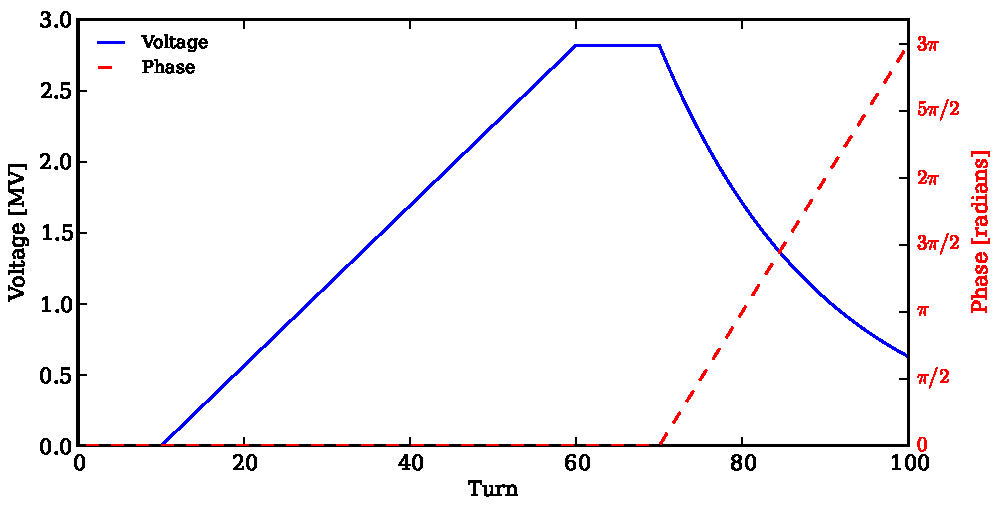
\includegraphics{fail_voltagePhase2v2}
  \caption{Singals generate by DYNK example for ramp + exponential decay of crab voltage, and also linear drift of crab phase. Only the signals for CRAB\_IP1\_L1 are shown. The plot is made from the data in dynksets.dat.}
  \label{fig:DYNK_fail}
\end{figure}

This slightly more complicated example builds on the example given above.
It shows how to change two parameters (voltage and phase) of several objects.
It also demonstrates how functions can be chained together, making more complicated functions.
Some of the resulting functions are shown in Figure~\ref{fig:DYNK_fail}, and the DYNK block here looks like:
\begin{verbatim}
DYNK
/DEBUG
FUN zero CONST 0.0
FUN CV_R1 GET CRAB_IP1_R1 voltage
FUN CV_R2 GET CRAB_IP1_R2 voltage
FUN CV_R3 GET CRAB_IP1_R3 voltage
FUN CV_R4 GET CRAB_IP1_R4 voltage
FUN CV_L  GET CRAB_IP1_L1 voltage
FUN ramp LIN 0.02 0
FUN ramp_R1 MUL CV_R1 ramp
FUN ramp_R2 MUL CV_R2 ramp
FUN ramp_R3 MUL CV_R3 ramp
FUN ramp_R4 MUL CV_R4 ramp
FUN ramp_L  MUL CV_L  ramp
SET CRAB_IP1_R1 voltage zero 1 10 0
SET CRAB_IP1_R2 voltage zero 1 10 0
SET CRAB_IP1_R3 voltage zero 1 10 0
SET CRAB_IP1_R4 voltage zero 1 10 0
SET CRAB_IP1_L1 voltage zero 1 9 0
SET CRAB_IP1_L2 voltage zero 1 9 0
SET CRAB_IP1_L3 voltage zero 1 9 0
SET CRAB_IP1_L4 voltage zero 1 9 0
/
SET CRAB_IP1_R1 voltage ramp_R1 11 61 -11
SET CRAB_IP1_R2 voltage ramp_R2 11 61 -11
SET CRAB_IP1_R3 voltage ramp_R3 11 61 -11
SET CRAB_IP1_R4 voltage ramp_R4 11 61 -11
SET CRAB_IP1_L1 voltage ramp_L 10 60 -10
SET CRAB_IP1_L2 voltage ramp_L 10 60 -10
SET CRAB_IP1_L3 voltage ramp_L 10 60 -10
SET CRAB_IP1_L4 voltage ramp_L 10 60 -10
/
/Voltage decay and detuning
FUN expCore LIN -0.05 0.0
FUN decay EXP expCore
FUN decayScaled MUL decay CV_L
SET CRAB_IP1_L1 voltage decayScaled 70 100 -70
SET CRAB_IP1_L2 voltage decayScaled 70 100 -70
SET CRAB_IP1_L3 voltage decayScaled 70 100 -70
SET CRAB_IP1_L4 voltage decayScaled 70 100 -70
FUN phasedrift LIN 0.3141592654 0.0
SET CRAB_IP1_L1 phase phasedrift 70 100 -70
SET CRAB_IP1_L2 phase phasedrift 70 100 -70
SET CRAB_IP1_L3 phase phasedrift 70 100 -70
SET CRAB_IP1_L4 phase phasedrift 70 100 -70
NEXT
\end{verbatim}
The first functions defined here are the same as above, storing the default values (as defined in the single element list) for the relevant elements and also zero.
Then follows a normalized linear ramp function ``ramp'', with gradient 0.02 = 1/50.
This is then used by the ``specialized'' ramp functions ``ramp\_R1$\cdots$R4'', which scales ``ramp'' so that the end point is the standard voltages for $t\in 0\ldots50$.

These functions are used to first set the crabs to 0.0 for the first 9 revolutions, and in the 10th revolution the ramp starts.
As the ``ramp'' function is defined starting at turn 0, a shift -10 or -11 is applied to the ramps.
The ramp is switched off after turn 60/61, leaving the crabs to be operating at the last SET value.

Further, we want to demonstrate a failure in the crab voltage.
This is done using an exponential decaying function $V(t) = V_0 \exp\left(-0.05 t\right)$, which is implemented as three chained functions:
\begin{description_alligned}{decayScaled}
\item[expCore] $f(t) = -0.05 t + 0.0$
\item[decay] $g(t) = \exp(f(t)) = \exp(-0.05 t + 0.0)$
\item[decayScaled] $h(t) = V_0 \cdot g(f(t)) = V_0 \cdot \exp(f(t)) = \exp(-0.05 t + 0.0)$
\end{description_alligned}
For the SET, the time $t$ is then shifted by -70 turns, so that the functions are evaluated starting at t=0.

\subparagraph{Detuning a cavity (accelerating or crab)}~\\
\todo[inline]{Write}

\subparagraph{Using the PIPE function}~\\
%Note: This example is referenced from the FUN table.

To use the PIPE functionality, add a FUN and SET to the DYNK block such as:
\begin{verbatim}
FUN pipe1 PIPE /tmp/pip1 /tmp/pip2 myID1 4242
SET  ACFCA.AR1.B1 voltage pipe1 10 -1 -9
\end{verbatim}
Then create the two pipes using the \texttt{mkfifo} UNIX command, e.g.\ \texttt{mkfifo~pip1} and \texttt{mkfifo~pip2} in the chosen directory.
When starting SixTrack, it will first open the input pipe (while reading the DYNK block), and wait for the external program to do the same.
This can be simulated by running \texttt{cat~>~pip1}; it is also possible to open the input pipe before starting SixTrack.
After opening the input pipe, SixTrack will open the output pipe, again this can be simulated by running \texttt{cat~pip2}, and again this pipe may be opened before starting SixTrack.
Note that when SixTrack ends, the output pipe will be closed, so the recieving \texttt{cat} process is terminated.

After opening the output pipe, SixTrack writes the line \texttt{DYNKPIPE~!******************!} to this file.
It then writes a line similar to \texttt{INIT~ID=myID1~for~FUN=pipe1} for each FUN using this output pipe.

During tracking, when one of the PIPE FUNs are called SixTrack writes a line similar to \texttt{GET ID=myID1 TURN=~1} to the output pipe.
Note that the turn number is the one passed to the FUN from SET, i.e. including any turn-shift.
It then waits for a single floating point number to be written (in ascii) to the input pipe, which is then read and returned from the FUN.

\subsection{Beam--Beam Element}
\label{BeamBeam}

\paragraph{Description} The beam--beam kick, including a separation of the beams, is treated \`{a} la Basetti and Erskine~\cite{BasErs} and implemented as in MAD~\cite{MAD}.
However, a much faster but nevertheless precise calculation using interpolation can be used~\cite{ERIC}.
For SixTrack version 3 the beam--beam is also available in the 6D form \`{a} la Hirata~\cite{Hirata}.
Lastly, the linear coupling has been considered in 4 and 6 dimensional phase space~\cite{ripbeam}. 

\paragraph{Keyword} BEAM
\paragraph{Number of data lines} variable but at least one

\paragraph{Format}
Two different input formats are available, ``traditional'' and ``EXPERT''.
If ``EXPERT'' mode is wanted, this is triggered by adding the flag \texttt{EXPERT} on the first line of the block.

\subparagraph{Traditional format}

\begin{itemize}
\item first data line: {\em partnum emitnx emitny sigz sige ibeco
    ibtyp lhc ibbc} 
\item other data lines: {\em name ibsix xang xplane xstr}
\end{itemize}

\begin{description}
\item [partnum] (float) Number of particles in bunch
\item [emitnx,emitny] (floats) Horizontal and vertical normalized
  emittance respectively [$\mu m\cdot rad$]
\item [sigz,sige] (floats) R.m.s. bunch length [m] and r.m.s. energy
  spread
\item [ibeco] (integer) Switch (0 = off; 1 = on) to subtract the
  closed orbit introduced by the separation of the beams. It is
  recommended to always subtract it as it is not yet calculated in a
  selfconsistent manner. The \emph{ibeco} switch also acts on the ``wire'' elements \ref{sec:WIRE} in the same way as on the beam-beam elements. It subtracts the closed orbit introduced by the wire if \emph{ibeco}=1 and applies it if \emph{ibeco}=0.
\item [ibtyp] (integer) Switch (0 = off; 1 = on) to use the fast
  beam--beam algorithms developed in collaboration with G.A.~Erskine
  and E.~McIntosh.  The linear optics are calculated with ``exact''
  beam--beam kicks.
\item [lhc] For the LHC with its anti--symmetric IR the separation of
  the beams in one plane can be calculated by the $\beta$--function of
  the other plane. For flat beams (not anti-symmetric optics) the separation
  can be loaded from the fort.2 file. (0 = off; 1 = anti-symmetric; 2 = load from file).
\item [ibbc] Linear coupling considered in 4D and 6D (0 = off; 1 = on).
\item [name] Name of 6D beam--beam element. Beam--beam elements that
  do not appear will be treated as 4D kicks.
\item [ibsix] (integer) Number of slices of the 6D beam--beam element.
  If {\it ibsix} is set to 0 this element is treated as a 4D element.
\item [xang] (float) Half crossing angle (angle the between the trajectories of the two beams) at this particular element [rad].
\item [xplane] (float) Crossing plane angle [rad].
\item [xstr] (float) Angle of the position of the slices in the boosted frame [rad] (i.e. $X = Z \sin(\mathit{xstr}) \cos(\mathit{xplane})$, $Y =Z \sin(\mathit{xstr}) \cos(\mathit{xplane})$ ).
  In absence of crabbing user should make sure \textit{xstr=xang}; in case the \textit{xstr} flag is not set then \textit{xstr=xang} is assumed and a warning is printed (since version 4.5.45).
\end{description}

\subparagraph{EXPERT format}

\begin{itemize}
\item first data line: {\em EXPERT}
\item second data line: {\em partnum emitnx emitny sigz sige ibeco
    ibtyp lhc ibbc} 
\item other data lines -- 4D BB lens (1 line per element): \\
{\em name ibsix $\Sigma_{xx}$ $\Sigma_{yy}$ h-sep v-sep strength-ratio}
\item other data lines -- 6D BB lens (3 lines per element): \\
{\em name ibsix xang xplane h-sep v-sep} \\
{\em $\Sigma_{xx}$ $\Sigma_{xxp}$ $\Sigma_{xpxp}$ $\Sigma_{yy}$ $\Sigma_{yyp}$} \\
{\em $\Sigma_{ypyp}$ $\Sigma_{xy}$ $\Sigma_{xpy}$ $\Sigma_{xpyp}$ $\Sigma_{yyp}$ strength-ratio} \\
\end{itemize}

Some parameters are new or defined in a different way:
\begin{description}
\item [lhc] This parameter is kept for now only for RHIC studies when equal to 9.
\item [name] Name of the beam--beam element.
\item [ibsix] (integer) Number of slices of the 6D beam--beam element.\\
  If {\it ibsix} is set to 0 this element is treated as a 4D element.\\
  If {\it ibsix} is larger or equal 1 this element is treated as a 6D element.
\item [$\Sigma_{xx}$] Horizontal $\sigma$ for the strong beam $\rm{[mm^2]}$.
\item [$\Sigma_{yy}$] Vorizontal $\sigma$ for the strong beam $\rm{[mm^2]}$.
\item [h-sep] Horizontal beam--beam separation [mm]
\item [v-sep] Vertical beam--beam separation [mm]
\item [strength-ratio] Strength ratio with respect to the nominal beam--beam kick strength.
  This is useful to allow for splitting one beam--beam kick into several (longitudinally close by) kicks.
\item [$\Sigma_{i,j}$] Second order momenta matrix for the strong beam, in units of mm and mrad.
  For example $\Sigma_{xxp}$ in [mm\ mrad]
\end{description}

\paragraph{Remark} These beam--beam elements have to appear in the single element list (~\ref{NonEle}) (type 20).
If the ``traditional'' option is used in the BEAM block, the listing in the single element list must contain their horizontal and vertical beam--beam separations (see~\ref{BBS}).

\paragraph{Sign Convention} Some clarifications regarding the sign convention used
for the separation and crossing angle variables.
\todo[inline]{Check if applies to both ``traditional'' and ``EXPERT'' format.}
\begin{itemize}
 \item Separations:
 \begin{enumerate}
  \item The separation is added to the transverse coordinates of each particles just before the beam-beam subroutines (see Fig.~\ref{fig:BB_sep}).
  \begin{eqnarray*}
   \tilde x_i=x_i+sep_x-CO_x \\
   \tilde y_i=y_i+sep_y-CO_y 
  \end{eqnarray*}
  \item Lorentz boost applied to the updated coordinates.
  \item The separation used for the actual beam-beam kick (sep$_{x,y,kick}$) is the difference between the centroid of the strong slice (X$^{\dag}$,Y$^{\dag}$) and the each particle (x$_i$,y$_i$).
  \item Antiboost to return to accelerator frame.
  \item The separation is removed and the closed orbit is added back. Tracking continues.
  \begin{eqnarray*}
   \tilde x_i=x_i-sep_x+CO_x \\
   \tilde y_i=y_i-sep_y+CO_y
   \end{eqnarray*}
 \end{enumerate}
 \begin{figure}[h]
 \begin{center}
 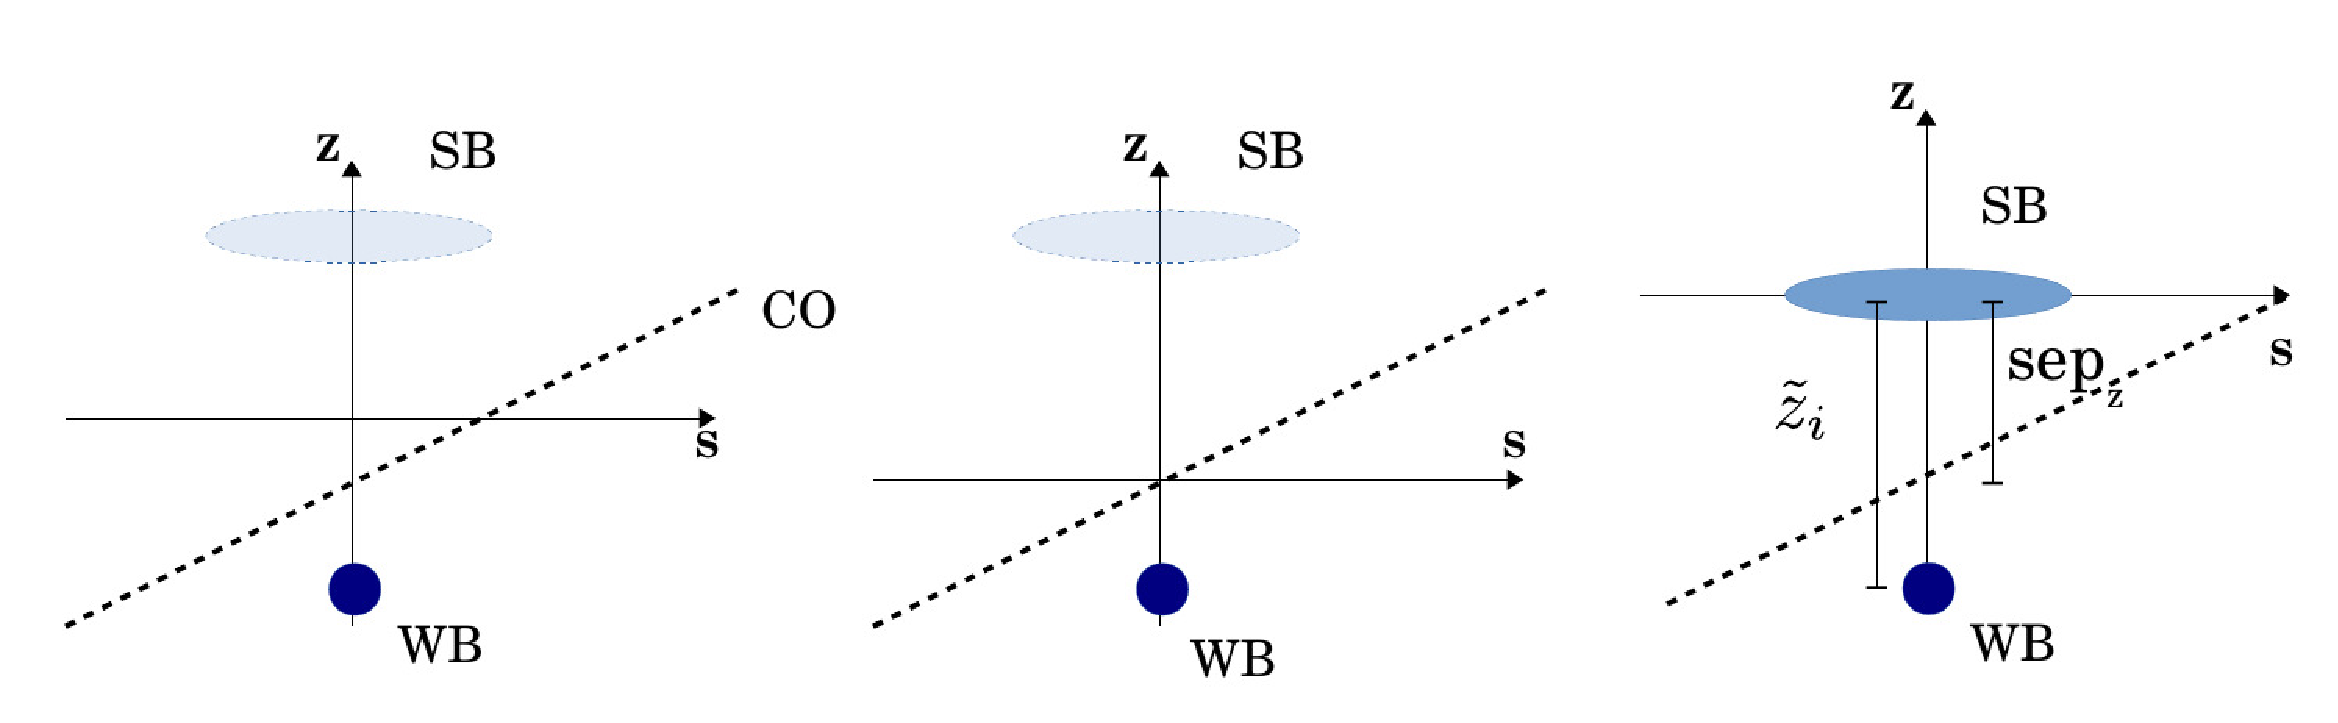
\includegraphics[width=0.8\textwidth]{BB_sep}
 \caption{Coordinate manipulation taking into consideration the beam-beam lens separation as stated in point 1 of the separation sign convention.}
 \label{fig:BB_sep}
 \end{center}
\end{figure}
 \item Crossing angles:
 \begin{enumerate}
  \item The closed orbit is removed just before the beam-beam subroutines.
  \begin{eqnarray*}
   \tilde x'_i=x'_i-CO_{x'} \\
   \tilde y'_i=y'_i-CO_{y'}
  \end{eqnarray*}
  \item Lorentz boost applied to the updated coordinates.
  \item Apply Synchro-Betatron Mapping.
  \item Antiboost to return to accelerator frame.
  \item The closed orbit is added back. Tracking continues.
  \begin{eqnarray*}
   \tilde x'_i=x'_i+CO_{x'} \\
   \tilde y'_i=y'_i+CO_{y'}
  \end{eqnarray*}
 \end{enumerate}
 \begin{figure}[h]
 \begin{center}
 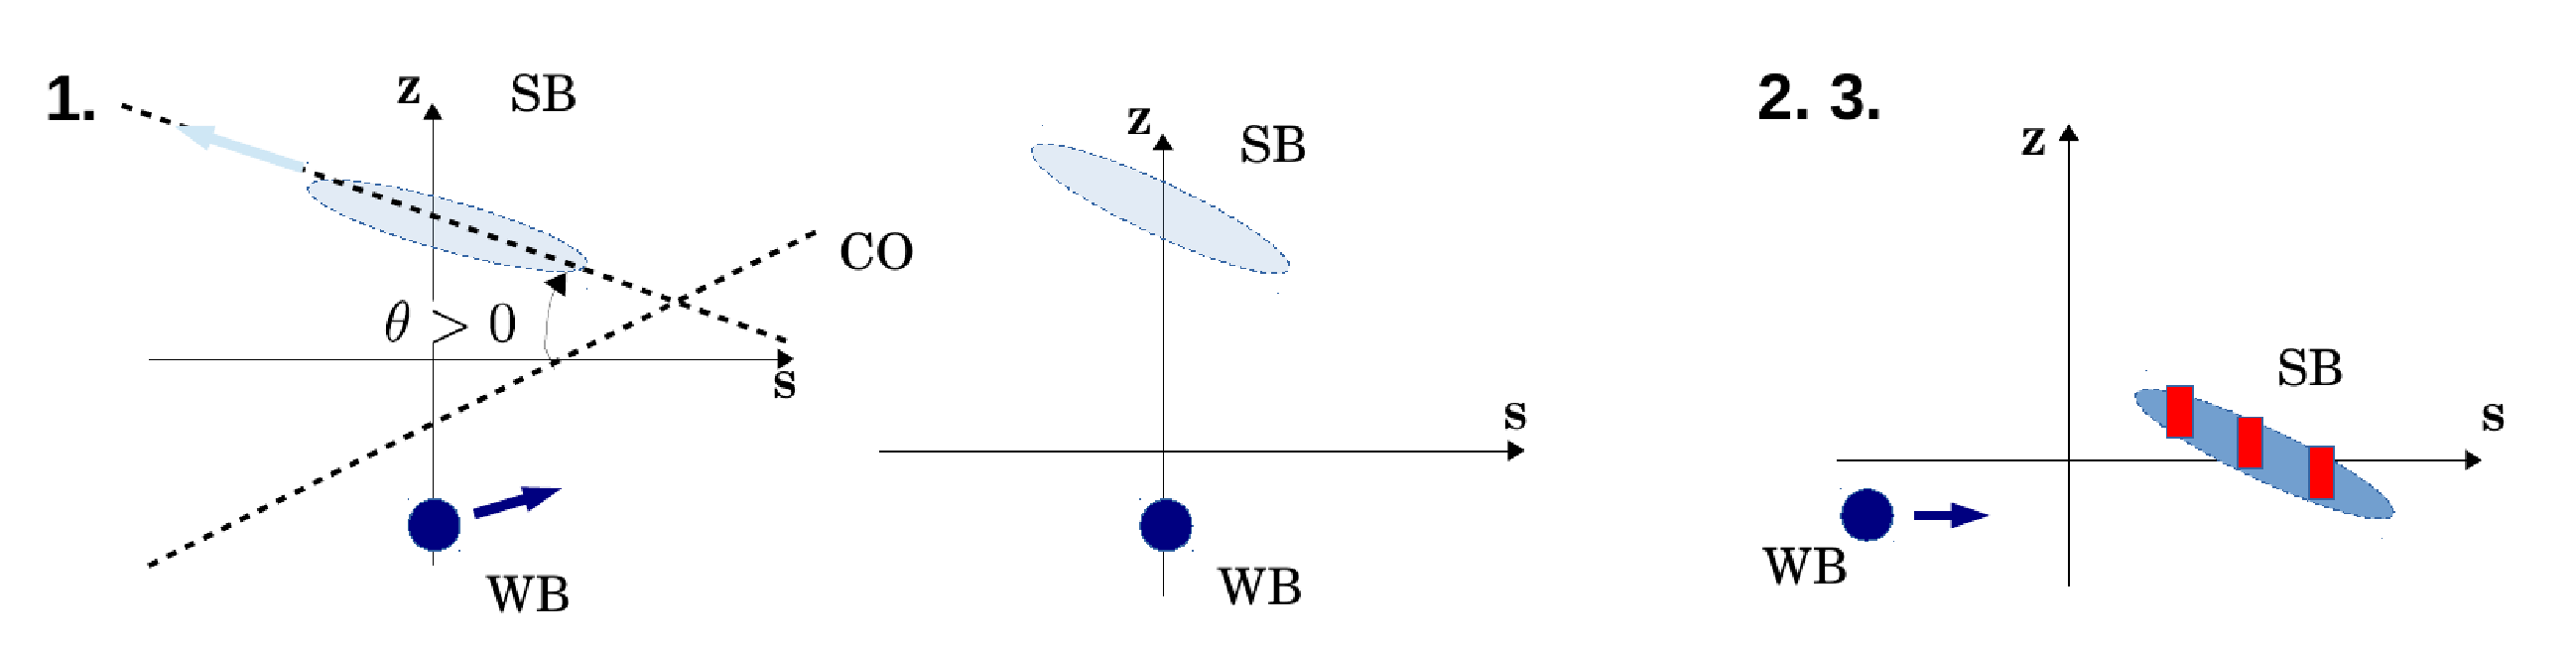
\includegraphics[width=0.8\textwidth]{BB_xsing}
 \caption{Coordinate manipulation to move from the accelerator frame to a head-on collision frame (Figures left and center). A positve crossing angle is considered as shown in the left figure.
 Then Lorentz boost and Synchro-Betatron Mapping are applied (right).}
 \label{fig:BB_xsing}
 \end{center}
\end{figure}
\end{itemize}

\subsection{Wire} \label{sec:WIRE}

\paragraph{Description} The wire block serves for reading in the input parameters for the wire. Each wire also needs to be added as single element in the list of single elements.

\paragraph{Keyword} WIRE

\paragraph{Number of data lines} variable

\paragraph{Format} \emph{name flag\_co current int\_length phys\_length disp\_x disp\_y tilt\_x tilt\_y}
A description of the input parameters for the wire is given in Table~\ref{tab:wire}.
\begin{center}
	\begin{longtable}{|p{2.0cm} p{1.0cm} p{9.2cm}|}
		%Note: \\* (with the star) used to inhibit page breaks in the middle of groups of the same type
		\caption{Input parameters for WIRE block.}
		\label{tab:wire} \\*
		\hline
		\rowcolor{blue!30}
		Arguments & unit & Description \\*
		\hline
		\endfirsthead
		
		\hline
		\rowcolor{blue!30}
		Arguments & unit & Description \\*
		%\hline
		\endhead
		
		\rowcolor{gray!15}
		\multicolumn{3}{|c|}{(The table continues on the next page)}\\*
		\hline
		\endfoot
		
		\hline
		\endlastfoot
		
		\hline
		
		\emph{name} & - &
		Name of wire. Must be the same as in list of single elements.\\*
		
		\emph{flag\_co} & - &
		flag to define the displacement of the wire in respect to the closed orbit or x=y=0. For \emph{flag\_co}=+1 \emph{disp\_*} is the distance between x=y=0 and the wire. For \emph{flag\_co}=-1 \emph{disp\_*} is the distance between the closed orbit and the wire.\\*
		\emph{current} & A &
		wire current \\*
		\emph{int\_length} & m &
		integrated length of the wire\\*
		\emph{phys\_length} & m &
		physical length of the wire\\*
		\emph{disp\_x} & mm &
		hor. displacement of the wire\\*
		\emph{disp\_y} & mm &
		vert. displacement of the wire\\*
		\emph{tilt\_x} & degrees &
		hor. tilt of the wire $-90 < tilt\_x < 90$ (uses same defintion as DISP block) \\*
		\emph{tilt\_y} & degrees &
		vert. tilt of the wire $-90 < tilt\_y < 90$ (uses same defintion as DISP block) \\*
		\hline		
	\end{longtable}
\end{center}

\paragraph{Remark} The user has to check that the wires defined in the WIRE block are also defined in the list of single elements and vice versa. All parameters except for the type (type 15) are ignored in the single element definition and the execution is aborted if the parameters are non-zero. In addition to the parameters defined in the WIRE block, the \emph{ibeco} parameter in the BEAM block (see Sec.~\ref{BeamBeam}) imposes the same behavior on the wire as for beam-beam. Explicitly, the closed orbit introduced by the wire is subtracted if \emph{ibeco}=1 and not subtracted if \emph{ibeco}=0.

\paragraph{Example} In the following we give some examples for wire definitions. This example defines two wires wire\_1 and wire\_2.

The input block in \verb|fort.3| is given by:
\begin{verbatim}
WIRE
wire_1   -1  +98.9   2.0  1.0   10.0   10.0     1.1     1.1
wire_2   -1  +98.9   2.0  1.0   10.0   10.0     0.0     0.0
NEXT
\end{verbatim}
The single and structure element definition in \verb|fort.2| is given by:
\begin{verbatim}
SINGLE ELEMENTS---------------------------------------------------------
...
wire_1           15   0.000000000e+00   0.000000000e+00 
0.000000000e+00    0.000000000e+00    0.000000000e+00    0.000000000e+00
wire_2           15   0.000000000e+00   0.000000000e+00 
0.000000000e+00    0.000000000e+00    0.000000000e+00    0.000000000e+00
...
STRUCTURE INPUT---------------------------------------------------------
...
BLOC56            wire_1              wire_2
...
\end{verbatim}
Note that all parameters except for the type have to be set to 0 in the single element definition.

\subsection{``Phase Trombone'' Element} \label{Trombone}

\subparagraph{Description} The linear ``phase trombone'' allows to
introduce a change in the tranverse phases without spoiling the linear
optics of the rest of the machine, i.e. the Twiss parameters are the
same at entrance and exit of the element.  
\subparagraph{Keyword} TROM
\subparagraph{Number of data lines} 1 line with name and then in
blocks of 14 lines with 3 entries each

\subparagraph{Format} 
\begin{itemize}
\item first data line: {\em name}
\item second data line: {\em cx, $cx'$, cy}
\item third data line: {\em $cy'$, cz, $cz'$}
\item fourth till $15^{th}$ {\em M($ 6 \times 6$)} matrix 
\end{itemize}

\begin{description}
\item [name] May contain up to sixteen characters
\item [cx, $cx'$, cy, $cy'$, cz, $cz'$] (floats) 6D closed orbit to be added
  to the coordinates.
\item [M($ 6 \times 6$)] (floats) $ 6 \times 6$ matrix elements
\end{description}

\subparagraph{Remark} The user has to make sure that the above stated
conditions are fulfilled. When using the $mad\_6t$~\cite{CONVERTOR}
converter from MAD8 to SixTrack this is guaranteed to be the case. Note
also that the crossterms between the transverse plains are not
considered for the time being.

\subsection{Electron lens} \label{sec:elen}

\paragraph{Description} The electron lens module serves for reading in the input parameters for different types of electron lenses. Each e-lens also needs to be added as single element in the list of single elements. Currently only the ideal hollow electron lens is implemented.

\paragraph{Keyword} ELEN

\paragraph{Number of data lines} variable

\paragraph{Format} \emph{name type thetamax r2 r2ovr1 offset\_x offset\_y flag\_entrance flag\_exit}
A description of the input parameters for the different e-lens types is given in Table~\ref{tab:elen}. Currently only the ideal hollow electron lens is implemented in SixTrack (type ANNULAR).
\begin{center}
	\begin{longtable}{|p{2.25cm} | p{2.0cm} p{1.0cm} p{9.2cm}|}
		%Note: \\* (with the star) used to inhibit page breaks in the middle of groups of the same type
		\caption{Input parameters for ELEN block.}
		\label{tab:elen} \\*
		\hline
		\rowcolor{blue!30}
		Type name & Arguments & unit & Description \\*
		\hline
		\endfirsthead
		
		\hline
		\rowcolor{blue!30}
		Type name & Arguments & unit & Description \\*
		%\hline
		\endhead
		
		\rowcolor{gray!15}
		\multicolumn{4}{|c|}{(The table continues on the next page)}\\*
		\hline
		\endfoot
		
		\hline
		\endlastfoot

		\hline
		\rowcolor{blue!15}
		\multicolumn{4}{|l|}{valid for all types} \\*
		
		& \emph{name} & - &
		Name of e-lens. Must be the same as in list of single elements.\\*
		
		& \emph{type} & - &
		type of electron lens. Available types are ANNULAR. \\*
		\hline

		\hline
		\rowcolor{blue!15}
		\multicolumn{4}{|l|}{type specific parameters} \\*
		
		ANNULAR & \emph{thetamax} & mrad &
		Maximum kick. This equals the kick received at $r=r_2$ where $r_2$ is the outer radius of the electron lens.\\*
		& \emph{r2} & mm &
		Outer radius of e-lens.\\*
		& \emph{r2ovr1} & - &
		Outer radius/inner radius.\\*
		& \emph{offset\_x} & mm &
		horizontal offset of e-lens.\\*
		& \emph{offset\_y} & mm &
		vertical offset of e-lens.\\*
		& \emph{flag\_entrance} & - &
		enable bends at entrance of e-lens.\\*
		& \emph{flag\_exit} & - &
		enable bends at exit of e-lens (not yet implemented).\\*
	\end{longtable}
\end{center}

\paragraph{Remark} The user has to check that the e-lens defined in the ELEN block is also defined in the list of single elements and vice versa. All parameters except for the type (type 29) are ignored in the single element definition.
The implementation of the ANNULAR type (ideal hollow e-lens) has no explicit energy-dependency, except for the user defined parameter \emph{thetamax} (see \cite{sixphys}).

\paragraph{Example} In the following we give some examples for e-lens definitions.

\subparagraph{ANNULAR} This example defines two electron lenses hel1 and hel2. The input block in \verb|fort.3| is then given by:
\begin{verbatim}
ELEN
hel1 ANNULAR 4.920e-03 6.928 1.5 0 0 0 0
hel2 ANNULAR 4.920e-03 6.928 1.5 1.1547 2.3093 0 0
NEXT
\end{verbatim}
The single and structure element definition in \verb|fort.2| is given by:
\begin{verbatim}
SINGLE ELEMENTS---------------------------------------------------------
...
hel1            29   0.000000000e+00   0.000000000e+00 
   0.000000000e+00    0.000000000e+00    0.000000000e+00    0.000000000e+00
hel2            29   0.000000000e+00   0.000000000e+00   
   0.000000000e+00    0.000000000e+00    0.000000000e+00    0.000000000e+00
...
STRUCTURE INPUT---------------------------------------------------------
...
BLOC56            hel1              hel2
...
\end{verbatim}
Note that all parameters except for the type are set to 0 in the single element definition.


\section{Organising Tasks}

In this section the input data blocks are described, which are used to
organise the input structure.

\subsection{Random Fluctuation Starting Number} \label{FluNum}

\subparagraph{Description} If besides mean values for the multipole
errors (Gaussian) random errors should be considered this input data
structure is used to set the start value for the random generator.

\subparagraph{Keyword} FLUC \subparagraph{Number of data lines} 1

\subparagraph{Format} {\em izu0 mmac mout mcut} \/(integers)
\begin{description}
\item [izu0] Start value for the random number generator
\item [mmac] {\em \large -- Sorry: disabled for the time being, i.e.\ 
    mmac is fixed to be 1 --} \/({\small In the vectorised version the
    number of different starting seeds can be varied.  Each seed is
    calculated as \mbox{$ k \times izu0 $} where $k$ runs from 1 to
    {\em mmac} \/which can not exceed 5 to save storage space (see
    list of parameters in Appendix~\ref{DSP}).})
\item {\em mout} A binary switch for various purposes, so all options,
  as described below, can be combined. 
\begin{itemize}
\item {\em mout} \/= 0 : multipole errors internally created
\item {\em mout} \/= 1 : multipole errors read--in from external file
  
  External multipole errors are read--in from file 16 into the array
  of random values. To activate these values one has to set to a value
  of 1 the relevant r.m.s.--positions of the corresponding multipole
  blocks (~\ref{MulCoe}). The systematic components are added as usual
  and multipoles not found in the fort.16 are treated as for ({\em
    mout} \/= 0 ). An error is only detected if there are too few sets
  of multipoles in fort.16.
\item {\em mout} \/= 2: the geometry and strength file is written to
  file \# 4 in the same format as the input file \# 2; the multipole
  coefficients are written to file \# 9; name, misalignments and tilt
  is written to file \# 27 and finally name, random single multipole
  strength and both random transverse misalignments are written to
  file \# 31.
\item {\em mout} \/= 4: Name, horizontal and vertical misalignment and
  also the element tilt are read--in from file \# 8.
\item {\em mout} \/= 8: Name and 3 Random numbers for single kick
  strength and both random transverse misalignments and also the value
  of the tilt are read--in from file \# 30. 
\end{itemize}
\item [mcut] The random distribution can be cut by {\em mcut} \/sigma
  of the distribution. No cuts are applied for {\em mcut = 0}\/.
\end{description}

\subparagraph{Remarks}
\begin{enumerate}
\item The RANECU random generator \cite{RANECU} is used as it produces
  machine independent sequences of random numbers.
\item If the starting point has to be changed or another nonlinear
  element is to be inserted, this can be done without changing the
  once chosen random distribution of errors by using the {\em
    Organisation of Random Numbers} \/input block.
\item The description of an accelerator is fully contained in 4 files:
  fort.2 (geometry), fort.3 (tracking parameters and definition of
  multipole blocks), fort.16 (multipole errors) and fort.30 (random
  numbers of the single multipole kick, the horizontal and vertical
  misalignment and the value of the tilt). This block allows to write
  out the files \# 4, 9, 27, 31 which may serve as the input files \#
  2, 16, 8 and 30 respectively. The file fort.30 superseeds fort.8 if
  both files are read in.
\end{enumerate}

\subsection{Organisation of Random Numbers} \label{OrgRan}

\subparagraph{Description} Working on a lattice for an accelerator
often requires to introduce new nonlinear elements. In those cases
simply introducing this new element means that the previously chosen
random distribution of the errors will be changed and with it often
the linear parameters. This input data block is mainly used to avoid
this problem by reserving extra random numbers for the new elements.
It also allows to change the observation point without affecting the
machine. The random values of different nonlinear elements including
blocks of multipoles can be set to be equal to allow to vary the
number of nonlinear kicks in one magnet which clearly should have the
same random distribution for each multipolar kick. Finally multipole
sets with different name can be made equal with this input data block.

\subparagraph{Keyword} ORGA \subparagraph{Number of data lines}
variable

\subparagraph{Format} {\em ele1 ele2 ele3} \/The data lines can be set
in three different ways:
\begin{enumerate}
\item Ele1 = ``name'' where name $\ne$ MULT \\
  Ele2 = ignored \\
  Ele3 = ignored \\
  The nonlinear element or multipole set will have its own set of
  random numbers.
\item Ele1 = ``name1'' where name1 $\ne$ MULT \\
  Ele2 = ``name2'' \\
  Ele3 = ignored \\
  The nonlinear element or multipole block Ele1 has the same random
  number set as those of Ele2, if it follows Ele2 as the first
  nonlinear element in the structure list (~\ref{StrInp}).
\item Ele1 = ``MULT'' \\
  Ele2 = ``name2'' \\
  Ele3 = ``name3'' \\
  The multipole set ``name3'' is set to the values of the set
  ``name2''. random errors are not influenced in this case.
\end{enumerate}

\subparagraph{Remarks}
\begin{enumerate}
\item A simple change of the starting point, by placing a ``GO''
  somewhere in structure, used to change the machine optics as the
  random numbers were shifted, too.  Simply calling this block even
  without a data line, will always fix the sequence of random numbers
  to start at the first multipole in the structure.
\item This input data block must follow the definition of the
  multipole block, otherwise multipoles cannot be set equal (option
  3).
\item Do not use the keyword ``MULT'' in the single element list
  (~\ref{SinEle}).
\end{enumerate}

\subsection{Combination of Elements} \label{ComEle}

\subparagraph{Description} It is often necessary to use several
families of magnetic elements with a certain ratio $ R $ of magnetic
strength to perform corrections like tune adjustment (~\ref{TunVar}),
chromaticity correction (~\ref{ChrCor}) or resonance compensation
(~\ref{ResCom}).  The {\em Combination of Elements} \/input block
allows such a combination of elements.  The maximum number of elements
is defined by the parameter NCOM (see Appendix~\ref{DSP}).

\subparagraph{Keyword} COMB \subparagraph{Number of data lines}
variable

\subparagraph{Format} {\em e0 R1 e1 \dots Rn en}

\begin{description}
\item [e0] Reference element which appears in the input of the
  processing procedure
\item [e1, \dots, en] Elements to be combined with {\em e0}
\item [Rj] Ratio of the magnetic strength of element {\em ej} \/to
  that of element {\em e0}
\end{description}

\section{Processing}

This section comprises all the input blocks that do some kind of pre--
or post--processing.

\subsection{Linear Optics Calculation} \label{LinOpt}

\subparagraph{Description} The linear optics calculation input block
is used to make a printout of all linear parameters (magnet lengths,
$\beta$ and $\alpha$ functions, tunes, dispersion and closed orbit) in
the horizontal and vertical planes at the end of each element or
linear block.  The number of elements or blocks can be chosen.

\subparagraph{Keyword} LINE \subparagraph{Number of data lines}
variable but at least 1

\subparagraph{Format}
\begin{itemize}
\item first data line: {\em mode number--of--blocks ilin ntco E\_I E\_II}
\item other data lines: {\em name(1), \dots , name(nlin)}
\end{itemize}


\begin{description}
\item [mode] ``ELEMENT'' for a printout after each single element
  (\ref{SinEle}); ``BLOCK'' for a printout after each structure block
  (\ref{BloDef})
\item [number--of--blocks] (integer) The number of the blocks in the
  structure to which the linear parameter will be printed. If this
  number is set to zero or is larger than the number of blocks, the
  complete structure will be calculated.
\item [ilin] (integer) Logical switch to calculate the traditional
  linear optics calculation in 4D ({\it 1 = ilin}) and with the DA
  approach 6D ({\it 2 = ilin}).
\item [ntco] (integer) A switch to write out linear coupling
  parameters.
 \begin{itemize}
 \item {\em ntco} \/= 0 : no write--out
 \item {\em ntco} \/$\neq$ 0 : write--out of all linear coupled (4D)
   parameters including the coupling angle.  These parameters (name,
   longitudinal position, the phase advances at that location, 4
   $\beta$--, $\alpha$-- and $\gamma$--functions, 4 angles for
   coordinates and momenta respectively, plus the coupling angle
   [rad]) are written in ascii format on file \# 11.
   This write-out happens every \emph{ntco} turns.
 \end{itemize}
\item [E\_I, E\_II] (floats) The two eigen--emittances to be chosen to
  determine the coupling angle. They are typically set to be equal.
\item [names] (char) For {\em nlin} \/($\leq $ {\em nele}\/) element--
  and block names the linear parameters are printed whenever they
  appear in the accelerator structure.
\end{description}

\subparagraph{Remarks}
\begin{enumerate}
\item To make this block work the Tracking Parameter block
  (~\ref{TraPar}) has to used as well.
\item When the ``ELEMENT 0'' option is used a file unit \# 34 is
  written with the longitudinal position, name, element type,
  multipole strength, $\beta$ functions and phase advances in the
  horizontal and vertical phase space respectively. This file is used
  as input for the ``SODD'' program~\cite{SODD} to calculate detuning
  and distortion terms in first and second order. A full program suite
  can be found at: /afs/cern.ch/group/si/slap/share/sodd
\item If the ``BLOCK'' option has been used, the tunes may be wrong by
  a multiple of 1/2. This option is not active in the DA part ({\it 2
    = ilin}), which also ignores the ({\it NTCO}) option.
\end{enumerate}

\subsection{Tune Variation} \label{TunVar}

\subparagraph{Description} This input block initializes a tune
adjustment with zero length quadrupoles.  This is normally done with
two families of focusing and defocusing quadrupoles. It may be
necessary, however, to have a fixed phase advance between certain
positions in the machine. This can be done with this block by
splitting the corresponding family into two sub--families which then
are adjusted to give the desired phase advance.

\subparagraph{Keyword} TUNE \subparagraph{Number of data lines} 2 or 4

\subparagraph{Format}
\begin{itemize}
\item data lines 1: {\em name1 Qx iqmod6}
\item data lines 2: {\em name2 Qy}
\item data lines 3 and 4, optional: {\em name3 $\Delta Q$} \/and {\em
    name4 name5} \/respectively
\end{itemize}

\begin{description}
\item [name1, name2] Names of focusing and defocusing quadrupole
  families respectively (in the single element list (~\ref{LinEle})
\item [Qx, Qy] (floats) Horizontal and vertical tune {\em including}
  \/the integer part
\item [iqmod6] (integer) Logical switch to calculate the tunes in the
  traditional manner ({\it 1 = iqmod6}) and with the DA approach
  including the beam-beam kick ({\it 2 = iqmod6}).
\item [name3] Name of the second sub--family, where the first
  sub--family is one of the above ({\em name1} \/or {\em name2}\/)
  This second sub--family replaces the elements of the first
  sub--family between the positions marked by {\em name4} \/and {\em
    name5}\/.
\item [$\Delta Q$] Extra phase advance {\em including} \/the integer
  part (horizontal or vertical depending on the first sub--family)
  between the positions in the machine marked by {\em name4} \/and
  {\em name5}
\item [name4, name5] Two markers in the machine for the phase advance
  $\Delta Q$ with the elements of the second sub--family between them
\end{description}

\subparagraph{Remark} The integer has to be included as the full phase
advance around the machine is calculated by the program.

\subsection{Chromaticity Correction} \label{ChrCor}

\subparagraph{Description} The chromaticity can be adjusted
to desired values with two sextupole family using this input block.

\subparagraph{Keyword} CHRO \subparagraph{Number of data lines} 2

\subparagraph{Format} data lines 1: {\em name1 $Q'_x$ ichrom}
\subparagraph{Format} data lines 2: {\em name2 $Q'_y$}

\begin{description}
\item [name1/2] Names (in the single element list (~\ref{NonEle}) of the
  two sextupole families
\item [$Q'$] Desired values of the chromaticity: $Q'=\frac{\delta
    Q}{\delta (\frac{\Delta p}{p_o})}$.
\item [ichrom] (integer) Logical switch to calculate the traditional
  chromaticity calculation ({\it 1 = ichrom}) and with the DA
  approach including the beam-beam kick ({\it 2 = ichrom}).
\end{description}
\subparagraph{Remark} To make the chromaticity correction work well a
small momentum spread is required (DE0 in table (~\ref{T-IteErr})). It
sometimes is required to optimize this spread.

\subsection{Orbit Correction} \label{OrbCorr}

\subparagraph{Description} Due to dipole errors in a real accelerator
a closed orbit different from the beam axis is unavoidable. Even after
careful adjustment one always will be left over with some random
deviation of the closed orbit around the zero position. A closed orbit
is introduced by nonzero strengths of $ b_{1} $ and $ a_{1} $
components of the multipole block (~\ref{MulCoe}), horizontal and
vertical dipole kicks (~\ref{NonEle}) or displacements of nonlinear
elements (~\ref{DisEle}).  This input data block allows the correction
of a such a random distributed closed orbit using he first two types
in a ``most effective corrector strategy'' \cite{Auti}. For that
purpose correctors have to be denoted by {\em ``HCOR= ''} \/and {\em
  ``VCOR= ''} \/and monitors by {\em ``HMON= ''} \/and {\em ``VMON=
  ''} \/for the horizontal and vertical plane respectively. After
correction the orbit is scaled to the desired r.m.s. values unless they
are zero.

On file unit 28 the horizontal orbit displacement, measured at the
horizontal monitors, will be written together with the monitor number,
on file unit 29 the same is done for the vertical closed orbit
displacement. 

\subparagraph{Keyword} ORBI \subparagraph{Number of data lines}
variable but at least 1

\subparagraph{Format}
\begin{itemize}
\item first data line: {\em sigmax sigmay ncorru ncorrep}
\item other data lines: {\em ``HCOR= '' namec} \/or {\em ``HMON= ''
    namem} \newline or {\em ``VCOR= '' namec} \/or {\em ``VMON= ''
    namem}
\end{itemize}

\begin{description}
\item [sigmax, sigmay] Desired r.m.s.--values of the randomly distributed
  closed orbit
\item [ncorru] Number of correctors to be used
\item [ncorrep] Number of corrections \newline If {\em ncorrep=0}
  \/the correction is iterated until {\em ITCO} \/(see
  table~\ref{T-IteErr}) iterations or after the both desired
  r.m.s.--values have been reached.
\item [``HCOR= '' namec] Horizontal correction element of name {\em
    namec}
\item [``HMON= '' namem] Horizontal monitor for the closed orbit of
  name {\em namem}
\item [``VCOR= '' namec] Vertical correction element of name {\em
    namec}
\item [``VMON= '' namem] Vertical monitor for the closed orbit of name
  {\em namem}
\end{description}

\subparagraph{Remarks}
\begin{enumerate}
\item Elements can have only one extra functionality: either
  horizontal corrector, horizontal monitor, vertical corrector or
  vertical monitor. If the number of monitors in a plane is smaller
  than the number of correctors it is likely to encounter numerical
  problems.
\item The {\em ``HCOR= ''}\/, {\em ``HMON= ''}\/, {\em ``VCOR= ''}
  \/and {\em ``VMON= ''} \/must be separated from the following name
  by at least one space.
\end{enumerate}

\subsection{Decoupling of Motion in the Transverse Planes}
\label{LinDec} 

\subparagraph{Description} Skew--quadrupole components in the lattice
create a linear coupling between the transverse planes of motion. A
decoupling can be achieved with this block using four independent
families of skew--quadrupoles, which cancel the off--diagonal parts of
the transfer map. As these skew--quadrupoles also influence the tunes
an adjustment of the tunes is performed at the same time.

\subparagraph{Keyword} DECO \subparagraph{Number of data lines} 3

\subparagraph{Format}
\begin{itemize}
\item first data line: {\em name1,name2,name3,name4}
\item data lines 2 and 3: {\em name5 Qx} \/and {\em name6 Qy}
  \/respectively
\end{itemize}

\begin{description}
\item [name1,2,3,4] Names of the four skew--quadrupole families
\item [name5, name6] Names of focusing and defocusing quadrupole
  families respectively (in the single element list (~\ref{LinEle})
\item [Qx, Qy] (floats) Horizontal and vertical tune {\em including}
  \/the integer part
\end{description}

\subparagraph{Remark} A decoupling can also be achieved by
compensating skew--resonances (~\ref{ResCom}).  The two approaches,
however, are not always equivalent. In the resonance approach the
zeroth harmonic is compensated, whilst a decoupling also takes into
account the higher--order terms.

\subsection{Sub--resonance Calculation} \label{SubCal}

\subparagraph{Description} First order resonance widths of multipoles
from second to ninth order are calculated following the approach of
Guignard \cite{Gilbert78}. This includes resonances, which are a
multiple of two lower than the order of the multipole. The first order
detuning including feed--down from closed orbit is calculated from all
multipoles up to to tenth order.

\subparagraph{Keyword} SUBR \subparagraph{Number of data lines} 1

\subparagraph{Format} {\em n1 n2 Qx Qy Ax Ay Ip length}

\begin{description}
\item [n1, n2] (integers) Lowest and highest order of the resonance
\item [Qx, Qy] Horizontal and vertical tune including the integer part
\item [Ax, Ay] Horizontal and vertical amplitudes in mm
\item [Ip] (integer) Is a switch to change the nearest distance to the
  resonance \mbox{$ e = nxQx + nyQy $.} In cases of structure
  resonances a change of $p$ by one unit may be useful.
 \begin{itemize}
 \item {\em ip} \/= 0 : $e$ is unchanged
 \item {\em ip} \/= 1 : \mbox{$ (e \pm 1) = nxQx + nyQy - (p \pm 1) $}
 \end{itemize}
\item [length] Length of the accelerator in meters
\end{description}

\subsection{Search for Optimum
  Places to Compensate Resonances} \label{SeaPla}

\subparagraph{Description} To be able to compensate a specific
resonance one has to know how a correcting multipole affects the
cosine and sine like terms of the resonance width at a given position
in the ring. This input data block can be used to find best places for
the compensation of up to three different resonances, by calculating
the contribution to the resonance width for a variable number of
positions. For each position the effect of a fixed and small change of
magnetic strength on those resonance widths is tested.

\subparagraph{Keyword} SEAR \subparagraph{Number of data lines}
variable but at least 2

\subparagraph{Format}
\begin{itemize}
\item data line 1: {\em Qx Qy Ax Ay length}
\item data line 2: {\em npos n ny1 ny2 ny3 ip1 ip2 ip3} \/(integers)
\item data lines from 3 on: {\em name1, \dots , namen}
\end{itemize}

\begin{description}
\item [Qx, Qy] Horizontal and vertical tune including the integer part
\item [Ax, Ay] Horizontal and vertical amplitudes in mm
\item [length] Length of the accelerator in m
\item [npos] Number of positions to be checked
\item [n] Order of the resonance
\item [ny1, ny2, ny3] Define three resonances of order $n$ via :
  \mbox{$ nx Qx + ny Qy = p $} with \mbox{$ \vert nx \vert + \vert ny
    \vert = n $}
\item [ip1,ip2,ip3] The distance to a resonance is changed by an
  integer $ip$ for each of the three resonances: \mbox{$ e = nx Qx +
    ny Qy - (p + ip) $.}
\item [namei] i'th name of a multipole of order $n$ , which has to
  appear in the single element list (~\ref{NonEle})
\end{description}

\subsection{Resonance Compensation} \label{ResCom}

\subparagraph{Description} The input block allows the compensation of
up to three different resonances of order $n$ simultaneously the
chromaticity and the tunes can be adjusted. For mostly academic
interest there is also the possibility to consider sub--resonances
which come from multipoles which are a multiple of 2 larger than the
resonance order $n$. However, it must be stated that the
sub--resonances depend differently on the amplitude compared to
resonances where the order of the resonances is the same as that of
the multipoles.

\subparagraph{Keyword} RESO \subparagraph{Number of data lines} 6

\subparagraph{Format}
\begin{itemize}
\item data line 1: {\em nr n ny1 ny2 ny3 ip1 ip2 ip3} \/(integers)
\item data line 2: {\em nrs ns1 ns2 ns3} \/(integers)
\item data line 3: {\em length Qx Qy Ax Ay}
\item data line 4: {\em name1, \dots, name6}
\item data line 5: {\em nch name7 name8}
\item data line 6: {\em nq name9 name10 Qx0 Qy0}
\end{itemize}

\begin{description}
\item [nr] Number of resonances (0 to 3)
\item [n] Order of the resonance, which is limited to {\em nrco} \/= 5
  (see list of parameters in Appendix~\ref{DSP}).
  
  \mbox{normal: $ 3 \le n \le nrco $; skew: $ 2 \le n \le nrco $}
\item [ny1, ny2, ny3] Define three resonances of order $n$ via :
  \mbox{$ nx Qx + ny Qy = p $} with \mbox{$ \vert nx \vert + \vert ny
    \vert = n $}
\item [ip1, ip2, ip3] The distance to the resonance $ e $ can be
  changed by an integer value: \newline \mbox{$ e = nx Qx + ny Qy -
    (p+ip) $.}
\item [nrs] Number of sub--resonances (0 to 3)
\item [ns1, ns2, ns3] Order of the multipole with \mbox{$ ns \le 9 $}
  and \mbox{$ (ns-n)/2 \in {\mathbf N} $}
\item [length] Length of the machine in meters
\item [Qx, Qy] Horizontal and vertical tune including the integer part
\item [Ax, Ay] Horizontal and vertical amplitudes in mm
\item [name1, \dots, name6] Names (~\ref{NonEle}) of the correction
  multipoles for the first, second and third resonance
\item [nch] (integer) Switch for the chromaticity correction (0 = off,
  1 = on)
\item [name7, name8] Names (~\ref{NonEle}) of the families of
  sextupoles to correct the chromaticity
\item [nq] (integer) Switch for the tune adjustment (0 = off, 1 = on)
\item [name9, name10] Names (~\ref{LinEle}) of the families of
  quadrupoles to adjust the tune
\item [Qx0, Qy0] Desired tune values including the integer part
\end{description}

\subsection{Differential Algebra} \label{DifAlg}

\subparagraph{Description} This input block initiates the calculation
of a one turn map using the LBL Differential Algebra
package~\cite{DALIE}.  The use of this block inhibits
post--processing. The same differential algebra tools allow a
subsequent normal form analysis (see \cite{Forest89}).  A
four--dimensional version integrated in SixTrack is available as
described in sections~\ref{Normal} and~\ref{Corrections}.

\subparagraph{Keyword} DIFF.  \subparagraph{Number of data lines} 1 or
2

\subparagraph{Format}
\begin{itemize}
\item data line 1: {\em nord nvar preda nsix ncor}
\item data line 2: {\em name(1),\ldots,name(ncor)}
\end{itemize}

\begin{description}
\item [nord] (integer) Order of the map
\item [nvar] (integer) Number of the variables (2 to 6).  {\em nvar}
  \/= 2,4,6 : two-- and four--dimensional transverse motion and full
  six--dimensional phase space respectively.  {\em nvar} \/= 5 :
  four--dimensional transverse motion plus the relative momentum
  deviation \mbox{$ \frac{\Delta p}{p_o} $} as a parameter.
\item [preda] Precision needed by the DA package, usually set to
  \mbox{{\em preda} \/= 1e-38}
\item [nsix] (integer) switch to calculate a $ 5 \times 6 $ instead of a $
  6 \times 6 $ map. This saves computational time and memory space, as the
  machine can be treated up to the cavity as five--dimensional (
  constant momentum ).

 \begin{itemize}
 \item {\em nsix} \/= 0 : $ 6x6 $ map
 \item {\em nsix} \/= 1 : $ 5x6 $ map \\
   ({\em nvar} \/must be set to 6; 6D closed orbit must not be
   calculated, i.e. \mbox{\em iclo6 = 0}~(\ref{IniCoo}) and the map
   calculation is stopped once a cavity has been reached and being
   evaluated.)
 \end{itemize}
\item [ncor] (integer) Number of zero--length elements to be
  additional parameters besides the transverse and/or longitudinal
  coordinates (i.e.\ two--, four--, five-- or six--dimensional phase
  space).
\item [name(i)] (char) {\em Ncor} \/names (~\ref{NonEle}) of
  zero--length elements (e.g dipole kicks, quadrupole kicks,
  sextupoles kicks etc.).
\end{description}

\subparagraph{Remarks}
\begin{itemize}
\item For {\em nsix = 1} \/the map can only be calculated till a
  cavity is reached.
\item If the 6D closed orbit is calculated, the $ 5x6 $ map can not be
  done, {\em nsix} \/is therefore forced to 0.
\item If nvar is set to 5, the momentum dependence is determined
  without the need for including a fake cavity. With other words: the
  linear blocks are automatically broken up into single linear
  elements so that the momentum dependence can be calculated.
\item If a DA map is needed at some longitudinal location one just has
  to introduce an element denoted ``DAMAP'' at that place in the
  structure, ``DAMAP'' has also to appear as a marker (zero length,
  element type = 0) in the single element list (~\ref{NonEle}).  This
  extra map is written to file \# 17.
\end{itemize}

\subsection{Normal Forms} \label{Normal}

\subparagraph{Description} All the parameters to compute the Normal
Form of a truncated one--turn map are given in the {\em Normal Form }
\/input block. Details on these procedures including the next
block~\ref{Corrections} can be found in reference \cite{Massimo}.

\subparagraph{Keyword} NORM \subparagraph{Number of data lines} 1

\subparagraph{Format}
\begin{itemize}
\item first data line: {\em nord nvar}
\end{itemize}

\begin{description}
\item [nord] (integer) Order of the Normal Form
\item [nvar] (integer) Number of variables
\end{description}

\subparagraph{Remarks}
\begin{itemize}
\item The {\em Normal Form } \/input block has to be used in
  conjunction with the {\em Differential Algebra } \/input block that
  computes the one--turn map of the accelerator.
\item The value of the parameter {\em nord} \/should not exceed the
  order specified for the transfer map plus one.
\item The value of the parameter {\em nvar} \/should be equal to the
  number of coordinates used to compute the map plus eventually the
  number of correctors specified in the {\em Differential Algebra }
  \/input block.
\item the value $1$ for the off--momentum order is forbidden. This
  case corresponds to the linear chromaticity correction. It is in
  fact corrected by default when $par1 =1$ or $par2 =2$.
\end{itemize}

\subsection{Corrections} \label{Corrections}

\subparagraph{Description} All the parameters to optimise the
tune--shift using a set of correctors are given in the {\em Correction
  } \/input block. (For details see reference \cite{Massimo}.)

\subparagraph{Keyword} CORR \subparagraph{Number of data lines} 3

\subparagraph{Format}
\begin{itemize}
\item first data line: {\em ctype ncor}
\item second data line: {\em name(1),\ldots,name(ncor)}
\item third data line: {\em par1,\ldots,par5}
\end{itemize}

\begin{description}
\item [ctype] (integer) Correction type :
\begin{itemize}
\item ctype = 0 order--by--order correction
\item ctype = 1 global correction
\end{itemize}
\item [ncor] (integer) Number of zero--length elements to be used as
  correctors in the optimisation of the tune--shift.
\item [name(i)] (char) {\em Ncor} \/names of zero--length elements
  (e.g sextupoles kicks, octupoles kicks etc.).
\item [par1,\ldots,par5] Parameters for the correction. Their meaning
  depend on the value of {\em ctype} \/and is explained in Table \ref{tab:CORR}.
\end{description}
\begin{table}
\begin{center}
\caption{Tune-shift correction parameters}
\label{tab:CORR}
\begin{tabular}{|c|c|c|c|c|c|}
  \hline
  & & & & & \\
  & par1 & par2 & par3 & par4 & par5 \\
  & & & & & \\
  \hline
  & & & & & \\
  variable type & integer & integer & real & real & real \\
  & & & & & \\
  \hline
  & & & & & \\
  ctype = 0 & tune--shift & off--momentum & 0.0 & 0.0 & 0.0 \\
  & order $\leq 2 $& order $\leq 3 $& & & \\
  & & & & & \\
  \hline
  & & & & & \\
  ctype = 1 & $N_{min}\geq 2$ & $N_{max}\leq 3$ & $\alpha_H$ &
  $\alpha_V$ &
  $\delta_0 $ \\
  & & & & & \\
  \hline
\end{tabular}
\end{center}
\end{table}
\subparagraph{Remarks}
\begin{itemize}
\item The names of the elements specified in the {\em Correction }
  \/input block should be grouped according to the multipole type:
  first sextupoles, then octupoles $\ldots$ etc.\ 
\item In case of order--by--order corrections, at least one of the
  quantities $par1,par2$ has to be zero, i.e.\ the correction of
  tune--shift terms depending on both amplitude and momentum is not
  allowed (as stated in the previous section).
\end{itemize}

\subsection{Post--processing} \label{PosPro}

\subparagraph{Description} It has been seen in the past that the
tracking data hold a large amount of information which should be
extracted for a thorough understanding of the nonlinear motion. It is
therefore necessary to store the tracking data turn by turn and
post--process it after the tracking has been finished. The following
quantities are calculated:
\begin{enumerate}
\item {\bf Lyapunov exponent analysis} This allows to decide if the
  motion is of regular or chaotic nature, and, in the later case, that
  the particle will ultimately be lost.  This is done with the
  following procedure:
 \begin{enumerate}
 \item Start the analysis where the distance in phase space of the two
   particles reaches its minimum.
 \item Study the increase in a double logarithmic scale so that the
   slope in a regular case is always one, while a exponential increase
   stays exponential when we have chaos.
 \item Average the distance in phase space to reduce local
   fluctuations, as we are interested in a long range effect.
 \item Make a weighted linear fit with an increasing number of
   averaged values of distance in phase space, so that an exponential
   increase results in a slope that is larger than one and is
   increasing. (The weighting stresses the importance of values at
   large turn numbers).
 \end{enumerate}
\item {\bf Analysis of the tunes} This is done either by the averaged
  phase advance method leading to very precise values of the
  horizontal and vertical tunes. A FFT analysis is also done.  With
  the second method one can evaluate the relative strength of
  resonances, rather than achieve a precise tune measurement. In both
  cases the nearby resonances are determined.
\item {\bf Smear} The smear of the horizontal and vertical emittances
  and the sum of the emittances are calculated in case of linearly
  coupled and un--coupled motion.
\item {\bf Nonlinear Invariants} A rough estimate of the nonlinear
  invariants are given.
\item {\bf Plotting} The processed tracking data can be plotted in
  different ways:
 \begin{enumerate}
 \item The distance of phase space as a function of amplitude
 \item Phase space plots
 \item Stroboscoped phase space
 \item FFT amplitudes
 \end{enumerate}
\item {\bf Summary} The post--processing results for a complete
  tracking session with varying initial parameters are summarised in a
  table at the end of the run.
\end{enumerate}

\subparagraph{Keyword} POST \subparagraph{Number of data lines} 4

\subparagraph{Format}
\begin{itemize}
\item data line 1: {\em comment title}
\item data line 2: {\em iav nstart nstop iwg dphix dphiy iskip iconv
    imad cma1 cma2} \/(general parameters)
\item data line 3: {\em Qx0 Qy0 ivox ivoy ires dres ifh dfft}
  \/(parameters for the tune calculation)
\item data line 4: {\em kwtype itf icr idis icow istw iffw nprint
    ndafi} \/(integer parameters for the plotting)
\end{itemize}

\begin{description}
\item [iav] (integer) Averaging interval of the values of the distance
  in phase space. Typically a tenth of the total turn number should be
  used as this interval.
\item [nstart, nstop] (integers) Start and stop turn number for the
  analysis of the post--processing (0 0 = all data used).
\item [iwg] (integer) Switch for the weighting of the slope
  calculation of the distance in phase space (0 = off, 1 = on).
\item [dphix, dphiy] Horizontal and vertical angle interval in radians
  that is used to stroboscope phase space. This stroboscoping of one
  of the two phase space projections is done by restricting the angle
  in the other phase space respectively to lie inside $\pm$ {\em
    dphix} \/or $\pm$ {\em dphiy}.
\item [iskip] (integer) This parameter allows to reduce the number of
  data to be processed: only each {\em iskip} \/sample of data will be
  used.
\item [iconv] (integer) If {\em iconv} \/is set to 1 the tracking data
  are not normalised linearly. Sometimes it is necessary to compare
  normalised to unnormalised data as the later will be found in the
  real machine.
\item [imad] (integer) This parameters is useful when MAD data shall
  be analysed ({\em imad} \/set to one).
\item [cma1, cma2] (floats) To improve the Lyapunov analysis for MAD
  data and in the case that the motion is 6D but the 6D closed orbit
  is not calculated the off--momentum and the path--length difference
  ($\sigma = s - v_o \times t$) can be scaled with {\em cma1} \/and
  {\em cma2} \/respectively (see also~\ref{SynOsc}). Please set both
  to 1.  when the 6D closed orbit is calculated.
\item [Qx0, Qy0] (floats) Values of the horizontal and vertical tune
  respectively (integer part) to be added to the averaged phase
  advance and to the $Q$ values of the FFT analysis.
\item [ivox, ivoy] (integers) The tunes from the average phase advance
  are difficult to be calculated when this phase advance is strongly
  changing from turn to turn and when the tune is close to 0.5, as
  then the phase may become negative leading to a deviation of one
  unit. This problem can partly be overcome by setting these switches
  in the following way:
 \begin{itemize}
 \item tune close to an integer: {\em ivox, ivoy} \/= 1
 \item tune close to half an integer: {\em ivox, ivoy} \/= 0
 \end {itemize}
\item [ires, dres] (integer,float) For the calculated tune values from
  the average phase advance method and the FFT--routine the closest
  resonances are searched up to {\em ires}\/'th order and inside a
  maximum distance to the resonance {\em dres}\/, so that \mbox{$ nx
    Qx + ny Qy < dres $ and $ nx + ny \le ires $.}
\item [ifh, dfft] (integer,float) For the FFT analysis the tune
  interval can be chosen with {\em ifh}\/.  To find resonances with
  the FFT spectrum, all peaks below a fraction {\em dfft} \/of the
  maximum peak are accepted.
 \begin{itemize}
 \item {\em ifh} \/= 0 : $ 0 \le Q \le 1 $
 \item {\em ifh} \/= 1 : $ 0 \le Q \le 0.5 $
 \item {\em ifh} \/= 2 : $ 0.5 \le Q \le 1 $
 \end{itemize}
\item [kwtype] {\large -- Disabled, set to 0 --} ({\small Terminal
    type, e.g. 7878 for the Pericom graphic terminals. For details,
    consult the HPLOT manual \cite{HPLOT}.})
\item [itf] Switch to get PS--file of plots
  \begin{itemize}
  \item {\em itf} = 0 : off
  \item {\em itf} = 1 : on
  \end{itemize}
\item [icr] {\large -- Disabled, set to 0 --} ({\small Switch to stop
    after each plot (0 = no stop, 1 = stop after each plot).}
\item [idis, icow, istw, iffw] Switches (0 = off) to select the
  different plots. If all values are set to zero, the HBOOK/HPLOT
  routine will not be called.
  \begin{itemize}
  \item {\em idis} \/= 1 : plot of distance in phase space
  \item {\em icow} \/= 1 : a set of plots of projections of the
    six--dimensional phase space and the energy E versus the turn
    number
  \item {\em istw} \/= 1 : plot of the stroboscoped phase space
    projection by restricting the phase in the other phase space
    projection
  \item {\em iffw} \/= 1 : plots of the horizontal and vertical FFT
    spectrum with linear amplitude scale
  \item {\em iffw} \/= 2 : plots of the horizontal and vertical FFT
    spectrum with logarithmic amplitude scale
  \end{itemize}
\item [nprint] Switch to stop the printing of the post--processing
  output to unit 6 (0 = printing off, 1 = printing on).
\item [ndafi] Number of data--files to be processed \mbox{(units :
    from 90 to (90--ndafi+1)\hspace{3mm}).}
\end{description}

\subparagraph{Remarks}
\begin{enumerate}
\item The post--processing can be done in two ways :
\begin{enumerate}
\item directly following a tracking run by adding this input block to
  the input blocks of the tracking
\item as a later run where the tracking parameter file (unit \# 3)
  consists of only the {\em Program Version} \/input
  block~\ref{ProVer} (using the {\em FREE} \/option) and of this input
  block specifying the post--processing parameters followed by {\em
    ENDE} \/as usual
\end{enumerate}
\item The HBOOK/HPLOT routines are only used at the start of the main
  program for initialisation and termination. The actual plots are
  done in the post--processing subroutine. The routines are activated
  only if at least one of the plotting parameters ({\em idis, icow,
    istw, iffw}\/) is set to one.
\end{enumerate}

\section{Initial Conditions for Tracking}

\subparagraph{Description} For the study of nonlinear system the
choice of initial conditions is of crucial importance. The input
structure for the initial conditions was therefore organise in such a
way as to allow for maximum flexibility. SixTrack is optimised to
reach the largest possible number of turns. In order to derive the
Lyapunov exponent and thereby to distinguish between regular and
chaotic motion, the particle has a close by companion particle.
Moreover, experience has shown that varying only the amplitude while
keeping the phases constant is sufficient to understand the nonlinear
dynamics, as a subsequent detailed post--processing allows to find the
dependence of the parameter of interest on these phases.

\subsection{Tracking Parameters} \label{TraPar}

\subparagraph{Description} All tracking parameters are defined with
this input block, the initial coordinates are generally set here, too.
A fine tuning of the initial condition is done with Initial
Coordinates block (~\ref{IniCoo}) and the parameters for the
synchrotron oscillation are given in block (~\ref{SynOsc})

\subparagraph{Keyword} TRAC \subparagraph{Number of data lines} 3

\subparagraph{Format}
\begin{itemize}
\item data line 1: {\em numl numlr napx amp(1) amp0 ird imc niu(1) niu(2) numlcp numlmax}
\item data line 2: {\em idy(1) idy(2) idfor irew iclo6} \/(integers)
\item data line 3: {\em nde(1) nde(2) nwr(1) nwr(2) nwr(3) nwr(4) ntwin ibidu iexact} \/(integers)
\end{itemize}

\begin{description}
\item [numl] (integer) Number of turns in the forward direction
\item [numlr] (integer) Number of turns in the backward direction
\item [napx] (integer) Number of amplitude variations (i.e.\ particle pairs)
\item [amp(1), amp0] (floats) Start and end amplitude (any sign) in
  the horizontal phase space plane for the amplitude variations. The
  vertical amplitude is calculated using the ratio between the
  horizontal and vertical emittance set in the {\em Initial
    Coordinates} \/block (~\ref{IniCoo}), where the initial phase in
  phase space are also set. Additional information can be found in the
  {\em Remarks}\/.
\item [ird] (integer) Switch for the type of amplitude variation. In
  case {\em napx} \/= 1 the amplitude nstart is used.
 \begin{itemize}
 \item {\em ird} \/= 0 : amplitudes are varied between the amplitudes
   {\em amp(1)} \/and {\em amp0} \/with equal increments:
   $$
   delta = (amp0-amp(1)) / (napx-1)
   $$
 \item {\em ird} \/= 1 : amplitude variation to find an estimate for
   the short term dynamic aperture. The amplitude is increased or
   decremented corresponding to stable motion or particle loss
   respectively.  The change of amplitude is reduced each iteration
   \mbox{$i \le (napx-1) $} to:
   $$
   delta = (amp0-amp(1)) / 2^{i}
   $$
 \end{itemize}
\item [imc] (integer) Number of variations of the relative momentum
  deviation \mbox{$ \frac{\Delta p}{p_o} $}.  The maximum value of the
  relative momentum deviation \mbox{$ \frac{\Delta p}{p_o} $} is taken
  from that of the first particle in the {\em Initial Coordinates}
  \/block (~\ref{IniCoo}).  The variation will be between \mbox{$ \pm
    \frac{\Delta p}{p_o} (\mathrm{max}) $} in steps of \mbox{$
    \frac{\Delta p}{p_o} (\mathrm{max}) $ / ({\em imc--1}\/).}
\item[niu(1), niu(2)] Unknown; default values are 0.
\item[numlcp] Checkpoint/restart version: How often to write checkpointing files.
\item[numlmax] Checkpoint/restart version: Maximum ammount of turns; default is $10^6$.
\item [idy(1), idy(2)] A tracking where one of the transversal motion
  planes shall be ignored is only possible when all coupling terms are
  switched off.  The part of the coupling that is due to closed orbit
  and other effects can be turned off with these switches.
 \begin{itemize}
 \item {\em idy(1), idy(2)} \/= 1 : coupling on
 \item {\em idy(1), idy(2)} \/= 0 : coupling to the horizontal and
   vertical motion plane respectively switched off
 \end{itemize}
\item [idfor] Usually the closed orbit is added to the initial
  coordinates. This can be turned off using {\em idfor}\/, for
  instance when a run is to be prolonged.
 \begin{itemize}
 \item {\em idfor} \/= 0 : closed orbit added
 \item {\em idfor} \/= 1 : initial coordinates unchanged
 \item {\em idfor} \/= 2 : prolongation of a run, taken the initial
   coordinates from unit \# 13
 \end{itemize}
\item [irew] To reduce the amount of tracking data after each
  amplitude and relative momentum deviation iteration \mbox{$
    \frac{\Delta p}{p_o} $} the binary output units 90 and lower (see
  Appendix~\ref{Files}) are rewound.  This is always done when the
  post--processing is activated (~\ref{PosPro}). For certain
  applications it may be useful to store all data. The switch {\em
    irew} \/allows for that.
 \begin{itemize}
 \item {\em irew} \/= 0 : unit 90 (and lower) rewound
 \item {\em irew} \/= 1 : all data on unit 90 (and lower)
 \end{itemize}
\item [iclo6] This switch allows to calculate the 6D closed orbit
  using the differential algebra package. It is ignored in the regular
  tracking versions. It is active in all versions that link to the
  Differential Algebra package. This 6D closed orbit can be calculated
  from any longitudinal position contrary to earlier versions.

 \begin{itemize}
 \item {\em iclo6} \/= 0 : switched off
 \item {\em iclo6} \/= 1 : calculated
 \item {\em iclo6} \/= 2 : calculated and added to the initial
   coordinates (~\ref{IniCoo}).
 \item {\em iclo6} \/= 5 or =6: like for {\em 1} \/and {\em 2} \/but
   in addition a guess closed orbit is read (in free format) from file
   unit \# 33.
 \end{itemize}
\item [nde(1)] Number of turns at flat bottom, useful for energy
  ramping.
\item [nde(2)] Number of turns for the energy ramping.  {\em
    numl}\/--{\em nde(2)} \/ gives the number of turns on the flat
  top. For constant energy with \mbox{$ nde(1) = nde(2) = 0 $} the
  particles are considered to be on the flat top.
\item [nwr(1)] Every {\em nwr(1)}\/'th turn the coordinates will be
  written on unit 90 (and lower) in the flat bottom part of the
  tracking.
\item [nwr(2)] Every {\em nwr(2)}\/'th turn the coordinates in the
  ramping region will be written on unit 90 (and lower).
\item [nwr(3)] Every {\em nwr(3)}\/'th turn at the flat top a write
  out of the coordinates on unit 90 (and lower) will occur.  For
  constant energy this number controls the amount of data on unit 90
  (and lower), as the particles are considered on the flat top.
\item [nwr(4)] In cases of very long runs it is sometimes useful to
  save all coordinates for a prolongation of a run after a possible
  crash of the computer.  Every {\em nwr(4)}\/'th turn the coordinates
  are written to unit 6.
\item [ntwin] For the analysis of the Lyapunov exponent it is usually
  sufficient to store the calculated distance of phase space together
  with the coordinate of the first particle ({\em ntwin} \/set to
  one). You may want to improve the 6D calculation of the distance in
  phase space with {\em sigcor, dpscor} \/(see~\ref{IniCoo}) when the
  6D closed orbit is not calculated with {\em iclo6} \/$\neq 2$. If
  storage space is no problem, one can store the coordinates of both
  particles ({\em ntwin} \/set to two). The distance in phase space is
  then calculated in the post--processing procedure
  (see~\ref{PosPro}). This also allows a subsequent refined Lyapunov
  analysis using differential--algebra and Lie--algebra techniques
  (\cite{Refine}).
\item [ibidu] Switch to creat or read binary dump of the full
  accelerator decription on file \# 32. The parameters relevant to
  tracking, i.e.\ {\em numl, amp0, amp(1), amp(2), damp, chi0, chid,
    rat, $x_1$, $x'_1$, $y_1$, $y'_1$, ${\sigma}_1$, $\frac{\Delta
      p}{p_{o1}}$, $x_2$, $x'_2$, $y_2$, $y'_2$, ${\sigma}_2$,
    $\frac{\Delta p}{p_{o2}}$, time0, time1}, are to be given via the
  tracking parameter file \# 3.
 \begin{itemize}
 \item {\em ibidu} \/= 1 : write dump
 \item {\em ibidu} \/= 2 : read dump
 \end{itemize}
\item [iexact] Switch to enable exact solution of the equation of motion into
  tracking and 6D (no 4D) optics calculations.
  \begin{itemize}
    \item {\em iexact} \/= 0 : approximated equation
              (e.g. $x'\simeq \frac{P_x}{P_0(1+\delta)}$,
                    $y'\simeq \frac{P_y}{P_0(1+\delta)}$);
    \item {\em iexact} \/= 1 : exact equation (e.g
      $x'\simeq \frac{P_x}{P_0\sqrt{(1+\delta)^2-P_x^2-P_y^2}}$,
      $y'\simeq \frac{P_y}{P_0\sqrt{(1+\delta)^2-P_x^2-P_y^2}}$ ).
 \end{itemize}
\end{description}

\subparagraph{Remarks}
\begin{enumerate}
\item This input data block is usually combined with the {\em Initial
    Coordinates} \/input block (~\ref{IniCoo}) to allow a flexible
  choice of the initial coordinates for the tracking.
\item For a prolongation of a run the following parameters have to be
  set :
\begin{itemize}
\item in this input block : idfor = 1
\item in the {\em Initial coordinates} \/input block :
\begin{enumerate}
\item itra = 0
\item take the end coordinates of the previous run as the initial
  coordinates (including all digits) for the new run.
\end{enumerate}
\end{itemize}
\item A feature is installed for a prolongation of a run by using
  \mbox{\em idfor = 2} \/and 
  reading the initial data from unit \# 13. The end coordinates are
  now written on unit \# 12 after each run. Intermediate coordinates
  are also written on unit \# 12 in case the turn number \mbox{\em
    nwr(4)} \/is exceeded in the run. The user takes responsibility to
  transfer the required data from unit \# 12 to unit \# 13 if a
  prolongation is requested.
\item Some illogical combinations of parameters have been suppressed.
\item The initial coordinates are calculated using a proper linear 6D
  transformation: {\em amp(1)} \/is still the maximum horizontal
  starting amplitude (excluding the dispersion contribution) from
  which the emittance of mode 1 $e_I$ is derived, {\em rat}
  \/(see~\ref{IniCoo}) is the ratio of $e_{II}/e_I$ of the emittances
  of the two modes. The momentum deviation $\frac{\Delta p}{p_{o1}}$ is used to
  define a longitudinal amplitude. The 6 normalized coordinates read:
\begin{itemize}
\item horizontal:\\

  $\sqrt{e_I}=\frac{amp(1)}
  {\sqrt{\beta_{xI}}+\sqrt{\left|rat\right|\times\beta_{xII}}}$,\\

  $0.$

\item vertical: \\

 $sign(rat)\times \sqrt{e_{II}}$, with $e_{II} =
 \left|rat\right|\times e_{I}$,\\

 $0.$

\item longitudinal: \\

$0.$,\\ 

$\frac{\Delta p}{p_{o1}} \times \sqrt{\beta_{sIII}}$

\end{itemize}
and are then transformed with the 6D linear transformation into real
space. Note that results may differ from those of older versions.
\end{enumerate}

\subsection{Initial Coordinates} \label{IniCoo}

\subparagraph{Description} The {\em Initial Coordinates} \/input block
is meant to manipulate how the initial coordinates are organise, which
are generally set in the tracking parameter block (~\ref{TraPar}).
Number of particles, initial phase, ratio of the horizontal and
vertical emittances and increments of \mbox{2 $\times$ 6} coordinates
of the two particles, the reference energy and the starting energy for
the two particles.

\subparagraph{Keyword} INIT \subparagraph{Number of data lines} 16

\subparagraph{Format}
\begin{itemize}
\item first data line: {\em itra chi0 chid rat iver}
\item data lines 2 to 16: {\em 15 initial coordinates as listed in Table}~\ref{T-IniCoo}
\end{itemize}

\begin{description}
\item [itra] (integer) Number of particles
 \begin{itemize}
 \item {\em itra} \/= 0 : Amplitude values of tracking parameter block
   (~\ref{TraPar}) are ignored and coordinates of data line 2--16 are
   taken. {\em itra} \/is set internally to 2 for tracking with two
   particles.  This is necessary in case a run is to be prolonged.
 \item {\em itra} \/= 1 : Tracking of one particle, twin particle
   ignored
 \item {\em itra} \/= 2 : Tracking the two twin particles
 \end{itemize}
\item [chi0] Starting phase of the initial coordinate in the
  horizontal and vertical phase space projections
\item [chid] Phase difference between first and second particles
\item [rat] Denotes the emittance ratio ($e_{II}/e_I$) of horizontal
  and vertical motion. For further information see the \emph{Remarks} of the TRAC input block in Section~\ref{TraPar}.
\item [iver] In tracking with coupling it is sometimes desired to
  start with zero vertical amplitude which can be painful if the
  emittance ratio {\em rat} \/is used to achieve it. For this purpose
  the switch {\em iver} \/has been introduced:
\begin{itemize}
\item {\em iver} \/= 0 : Vertical coordinates unchanged
\item {\em iver} \/= 1 : Vertical coordinates set to zero.
\end{itemize}
\end{description}

\begin{table}
\caption{Initial Coordinates of the 2 Particles}
\label{T-IniCoo}
\centering
\begin{tabular}{|l|l|}
  \hline
  data line & contents \\
  \hline
  2 & $x_1$ [mm] coordinate of particle 1 \\
  3 & $x'_1$ [mrad] coordinate of particle 1 \\
  4 & $y_1$ [mm] coordinate of particle 1 \\
  5 & $y'_1$ [mrad] coordinate of particle 1 \\
  6 & path length difference 1 ($ {\sigma}_1 = s - v_o \times t$) [mm]
  of
  particle 1 \\
  7 & $ \frac{\Delta p}{p_{o1}} $ of particle 1 \\
  8 & $x_2$ [mm] coordinate of particle 2 \\
  9 & $x'_2$ [mrad] coordinate of particle 2 \\
  10 & $y_2$ [mm] coordinate of particle 2 \\
  11 & $y'_2$ [mrad] coordinate of particle 2 \\
  12 & path length difference ($ {\sigma}_2 = s - v_o \times t$) [mm]
  of
  particle 2 \\
  13 & $ \frac{\Delta p}{p_{o2}} $ of particle 2 \\
  14 & energy [MeV] of the reference particle \\
  15 & energy [MeV] of particle 1 \\
  16 & energy [MeV] of particle 2 \\
  \hline
\end{tabular}
\end{table}

\subparagraph{Remarks}
\begin{enumerate}
\item These 15 coordinates are taken as the initial coordinates if
  {\em itra} \/is set to zero (see above). If {\em itra} \/is 1 or 2
  these coordinates are added to the initial coordinates generally
  defined in the tracking parameter block (~\ref{TraPar}). This
  procedure seems complicated but it allows freely to define the
  initial difference between the two twin particles. It also allows in
  case a tracking run should be prolonged to continue with precisely
  the same coordinates. This is important as small difference may lead
  to largely different results.
\item The reference particle is the particle in the centre of the
  bucket which performs no synchrotron oscillations.
\item The energy of the first and second particles is given
  explicitly, again to make possible a continuation that leads
  precisely to the same results as if the run would not have been
  interrupted.
\item There is a refined way of prolonging a run, see the \mbox{\em
    Tracking Parameters} \/input block (~\ref{TraPar}).
\end{enumerate}

\subsection{Synchrotron Oscillation} \label{SynOsc}

\subparagraph{Description} The parameters needed for treating the
synchrotron oscillation in a symplectic manner are given in the {\em
  Synchrotron Oscillation} \/input block.

\subparagraph{Keyword} SYNC \subparagraph{Number of data lines} 2

\subparagraph{Format}
\begin{itemize}
\item first data line: {\em harm alc u0 phag tlen pma ition dppoff}
\item second data line: {\em dpscor sigcor}
\end{itemize}

\begin{description}
\item [harm] Harmonic number
\item [alc] Momentum compaction factor, used here only to calculate
  the linear synchrotron tune $ Q_{S} $.
\item [u0] Circumference voltage in [MV]
\item [phag] Acceleration phase in degrees
\item [tlen] Length of the accelerator in meters
\item [pma] rest mass of the particle in $ \mathrm{MeV}/\mathrm{c}^{2}
  $
\item [ition] (integer) Transition energy switch
 \begin{itemize}
 \item {\em ition} = \hspace{.3mm} 0 for no synchrotron oscillation
   (energy ramping still possible)
 \item {\em ition} = \hspace{.5mm} 1 for above transition energy
 \item {\em ition} = --1 for below transition energy
 \end{itemize}
\item [dppoff]  Offset Relative Momentum Deviation \mbox{$ \frac{\Delta
      p}{p_o} $}: a fixpoint with respect to synchrotron oscillations.
  It becomes active when the 6D closed orbit is calculated (see item
  {\it iclo6} \/in section~\ref{TraPar}).
\item [dpscor, sigcor] Scaling factor for relative momentum deviation
  \mbox{$ \frac{\Delta p}{p_o} $} and the path length difference
  ($\sigma = s - v_o \times t$) respectively.  They can be used to
  improve the calculation of the 6D distance in phase space, but is
  only used when {\em ntwin = 1} \/in the tracking parameter input
  block~(\ref{TraPar}). Please set to 1 when the 6D closed is
  calculated.
\end{description}

\section{Extra output files}
For some studies, extra output from the simulation is desired.
How to do this is described below.

\subsection{Dumping of beam population} \label{sec:DUMP}

\paragraph{Description}
The DUMP block allows the beam population (i.e.\ the position in phase-space for all the particles) to be written to file.
This can be done in any SINGLE ELEMENTS which are directly mentioned in the STRUCTURE INPUT part of fort.2 (BLOCs cannot be used).
The particles are dumped just after the kick is applied, and how often to dump (every turn, every second turn, etc.) is user-selectable.
Please note that each single element can only be selected once; however it is possible to overcome this limitation by placing multiple markers with different names in the same position in the sequence (by editing fort.2).

\paragraph{Keyword}
DUMP

\paragraph{Number of data lines}
variable, one for each element for which dump is active

\paragraph{Format}
\texttt{element\_name frequency unit format (filename) (first last)}\\
or \texttt{HIGH}\\
or \texttt{FRONT}

\subparagraph{element\_name}
one of the SINGLE ELEMENTS or ALL to dump at the exit of all single elements.
\subparagraph{frequency}
how often the beam population should be dumped in number of turns.
\subparagraph{unit}
fortran unit number to use, should not be used in other parts of SixTrack.
The unit number and filename may be shared between different DUMP outputs, as long as they have the same format and \texttt{element\_name} is not \texttt{ALL}.
\subparagraph{format}
an integer specifying the output format.
The following formats are accepted:
\begin{enumerate}
	\item[0] -- \textbf{General format:}\\
	No header\\
	Lines: \texttt{turn structure\_element\_idx single\_element\_idx single\_element\_name s x1[m] x1'[rad] y1[m] y2'[rad] momentum[GeV/c] dE/E[GeV]}
	\item[1] -- \textbf{Format for aperture check:}\\
	Header: \texttt{\# ID turn s[m] x[mm] xp[mrad] y[mm] yp[mrad] dE/E ktrack}\\
	Lines: \texttt{particleID turn s[m] x[mm] xp[mrad] y[mm] yp[mrad] dE/E ktrack}
	\item[2] -- \textbf{Modified format for aperture check:}\\
	Header line 1 (single element): \texttt{\# DUMP format \#2, bez=\textit{bez(i)}, number of particles=\textit{napx}, dump period=\textit{ndumpt(i)}, first turn=\textit{dumpfirst(i)}, last turn=\textit{dumplast(i)}, HIGH=\textit{T/F}, FRONT=\textit{T/F}}\\
	Header line 1 (all elements): \texttt{\# DUMP format \#2, ALL ELEMENTS, number of particles=\textit{napx}, dump period=\textit{ndumpt(i)}, first turn=\textit{dumpfirst(i)}, last turn=\textit{dumplast(i)}, HIGH=\textit{T/F}, FRONT=\textit{T/F}}\\
        Here \textit{bez} is the name of the SINGLE ELEMENT, and \textit{napx} the number of particles being tracked (per pack in case of collimation), \textit{ndumpt(i)} the dump frequency as described above, and \textit{dumpfirst(i)} and \textit{dumplast(i)} the first and last turn as descirbed below.
        HIGH and FRONT is normally false, unless this (global) option is active, as described below.\\
	Header line 2: \texttt{\# ID turn s[m] x[mm] xp[mrad] y[mm] yp[mrad] z[mm] dE/E ktrack}\\
        If there are multiple single elements attached to the file, the headers are repeated.\\
	Data lines: as described in the header, one per particle and per turn.
        \item[3] -- \textbf{Modified format for aperture check (Binary):}\\
        No header\\
        A number of Fortran records describing which elements are used and the current dump period is added one per relevant line in DUMP block.\\
        Records: \texttt{particleID turn s[m] x[mm] xp[mrad] y[mm] yp[mrad] z[mm] dE/E ktrack}\\
        The Fortran code \texttt{SixTest/readDump3/readDump3.f90} can be used to convert these files into the format 2 (sans headers).
	\item[4] -- \textbf{Beam means:}\\
        Header line 1 is the same as for format 2.\\
        Header line 2: \texttt{\# napx turn s[m] <x>[mm] <xp>[mrad] <y>[mm] <yp>[mrad] <z>[mm] <dE/E>[1]}\\
        If there are multiple single elements attached to the file, the headers are repeated.\\
        Data lines: As described in the header; one per turn (and for collimation, one per pack of particles).
	\item[5] -- \textbf{Beam mean and sigma:}\\
        Header line 1 is the same as for format 2.\\
	Header: \texttt{\# napx turn s[m] <x>[mm] <xp>[mrad] <y>[mm] <yp>[mrad] <z>[mm] <dE/E>[1] <x\^{}2> <x*xp> <x*y> <x*yp> <x*z> <x*(dE/E)> <xp\^{}2> <xp*y> <xp*yp> <xp*z> <xp*(dE/E)> <y\^{}2> <y*yp> <y*z> <y*(dE/E)> <yp\^{}2> <yp*z> <yp*(dE/E)> <z\^{}2> <z*(dE/E)> <(dE/E)\^{}2>}\\
        If there are multiple single elements attached to the file, the headers are repeated.\\
	A number of lines describing which elements are used and the current dump period is added one per relevant line in DUMP block.\\
	Data lines: As described in the header; one per turn (and for collimation, one per pack of particles).
        For the ``product'' quantities, the units are the product of the units of the ``normal'' ones.
	\item[6] -- \textbf{Beam mean and sigma (canonical):}\\
        Header line 1 is the same as for format 2.\\
	Header: \texttt{\# napx turn s[m] <x>[m] <px>[1] <y>[m] <py>[m] <sigma>[m] <psigma>[1] <x\^{}2> <x*px> <x*y> <x*py> <x*sigma> <x*psigma> <px\^{}2> <px*y> <px*py> <px*sigma> <px*psigma> <y\^{}2> <y*py> <y*sigma> <y*psigma> <py\^{}2> <py*sigma> <py*psigma> <sigma\^{}2> <sigma*psigma> <psigma\^{}2>}\\
        If there are multiple single elements attached to the file, the headers are repeated.\\
	A number of lines describing which elements are used and the current dump period is added one per relevant line in DUMP block.\\
	Data lines: As described in the header; one per turn (and for collimation, one per pack of particles).
        For the ``product'' quantities, the units are the product of the units of the ``normal'' ones.
        Note that the $\sigma=s -\beta_0 c t$ is the same as the $z$ used in the formats above, except for the unit of m instead of mm; and that $p_\sigma = \Delta E / \left(\beta_0 P_0 c\right)$.
        For more details, see the physics manual~\cite{sixphys}.
\end{enumerate}

\subparagraph{filename} is the name of the file to write to. This argument may be omitted (unless \texttt{first} and \texttt{last} are present, if so then \texttt{filename} must also be present), and if so the output file is named fort.\texttt{unit}.

\subparagraph{first} is the first turn where this dump should be active. This argument may be omitted if \texttt{last} is also omitted, and if so it defaults to turn 1.

\subparagraph{last} is the last turn where this dump should be active, -1 meaning ``untill the end of the simulation''. This argument may be omitted if \texttt{first} is also omitted, and if so it defaults to -1.

\subparagraph{HIGH} If present anywhere in the DUMP block this triggers high-precission output, meaning more digits in the output files.

\subparagraph{FRONT} If present anywhere in the DUMP block, this keyword triggers the DUMPed particles to be dumped in front of the element, i.e.\ before the kick.
This works for all elements, including BLOCs, when combined with the ALL ``element name''.
Note that FRONT is not yet supported for thick tracking, and trying to use this combination will produce a run-time error.

\paragraph{Example}
\begin{verbatim}
DUMP
/ALL 1 663 2
/CRAB5 1 659 0
ip1 1 660 2 IP1_DUMP.dat
ip5 1 662 2
mqml.10l4.b1..1 1 661 2 MQ_DUMP.dat
NEXT
\end{verbatim}

\subsection{FMA analysis} \label{sec:FMA}

\paragraph{Description}
The FMA block generates the basic files needed for frequency map analysis (FMA). Explicitly, it returns one output file with calculated tunes and amplitudes for the files specified in the DUMP block, see Sec.~\ref{sec:DUMP}. For the calculation of the tunes ($Q_1$, $Q_2$ and $Q_3$) in normalized phase space, the normalization matrix is extracted from the LINE block (linear optics calculation in 6D, \ref{LinOpt}). The tunes $Q_1$, $Q_2$ and $Q_3$ are then calculated with the routine specified in the FMA block either in physical coordinates ($x$,$x'$,$y$,$y'$,$z$,$dE/E$) or normalized phase space coordinates and dumped to the file \verb|fma_sixtrack| together with the minimum, maximum and average normalized particle amplitudes and phases. 

\paragraph{Keyword}
FMA

\paragraph{Number of data lines}
variable, one for each file with particle amplitudes and tune calculation method

\paragraph{Format of input block}
The FMA block has to be proceeded by the LINE block (calculation of the normalization matrix) and the DUMP block (dump particle coordinates).
\begin{verbatim}
DUMP
element_name_1 1 unit_1 2 filename_1 first_turn_1 last_turn_1
element_name_2 1 unit_2 2 filename_2 first_turn_2 last_turn_3
NEXT
LINE
ELEMENT  0 2 1 emit_1 emit_2
NEXT
FMA
filename_1 method_1 fma_flag_norm_1
filename_2 method_2 fma_flag_norm_2
NEXT
\end{verbatim}
For the DUMP block (Sec.~\ref{sec:DUMP}) the frequency has to be 1 (dump every turn) and the file format has to be 2. For the linear optics calculation \ref{LinOpt}, the optics needs to be calculated at eatch element (mode ELEMENT), the number-of-blocks is then 0 and 6D linear optics calculation is required (\verb|ilin = 2|) in order to decouple the 6D motion. 

\subparagraph{filename}
one of the outputfiles specified in the FMA block preceding DUMP block.
\subparagraph{method}
method used to calculate the tune. Available methods are: \verb|TUNELASK|, \verb|TUNEFIT|, \verb|TUNENEWT1|, \verb|TUNEABT|, \verb|TUNEABT2|, \verb|TUNEFFT|, \verb|TUNEFFTI|, \verb|TUNENEWT|, \verb|TUNEAPA|. A short description of the different methods is given in Table~\ref{fma:tab:1}.
\subparagraph{fma\_flag\_norm}
flag for calculating the tunes with physical ($x$,$x'$,$y$,$y'$,$s$,$dp/p$) or normalized coordinates. The default is using normalized coordinates (\verb|fma_flag_norm=1|). For using physical coordinates explicitly set (\verb|fma_flag_norm=0|).

\begin{table}[H]
	\begin{center}
		\caption{Available tune calculation methods in SixTrack.}
		\label{fma:tab:1}
		\begin{tabularx}{\textwidth}{|l|l|X|}
			\hline
\textbf{Library} & \textbf{method} & \textbf{Description} \\\hline
PLATO \cite{plato1,plato2}
& TUNELASK &	Compute the tune of a 2d map by means of laskar method. A first indication of the position of the tune is obtained by means of a FFT. Refinement is obtained through a newton procedure.\\\cline{2-3}
& TUNEFIT &	Computes the tune using a modified apa algorithm. The first step consists of taking the average of the tune computed with the APA method, then a best fit is performed.\\\cline{2-3}
& TUNENEWT1 &	Computes the tune using a discrete version of laskar method. It includes a newton method for the search of the frequency.\\\cline{2-3}
& TUNENEWT &	Computes the tune using a discrete version of laskar method. It includes a newton method for the search of the frequency.\\\cline{2-3}
& TUNEABT &	Computes the tune using FFT interpolated method.\\\cline{2-3}
& TUNEABT2 &	Computes the tune using the interpolated FFT method with hanning filter.\\\cline{2-3}
& TUNEFFT &	Computes the tune as the FFT on a two dimensional plane, given n iterates of a map. The FFT is performed over the maximum mft which satifies $2^{\rm mft} <= n$, where the maximum number of iterates is fixed in the parameter n.\\\cline{2-3}
& TUNEFFTI &	Computes the tune as the FFT on a two dimensional plane, given n iterates of a map. The FFT is performed over the maximum mft which satifies $2^{\rm mft} <= n$. Then, the FFT is interpolated fitting the three points around the maximum using a Gaussian. The tune is computed as the maximum of the Gaussian.\\\cline{2-3}
& TUNEAPA &	Computes the tune as the average phase advance on a two dimensional plane, given n iterates of a map. \\\hline
	\end{tabularx}
\end{center}
\end{table}
\paragraph{Output file format}
The FMA block returns the output files \verb|NORM_filename*| containing the normalized phase space coordinates, where \verb|filename| are the filenames specified in the dump block, and the file \verb|fma_sixtrack| containing the initial, average, minimum and maximum amplitudes and the calculated tunes for each specified filename and method. The structure of the \verb|NORM_filename*| is described in Table~\ref{fma:tab:2} and of the \verb|fma_sixtrack| in Table~\ref{fma:tab:3}.
\begin{table}[H]
	\begin{center}
	\caption{Format of the NORM files}\label{fma:tab:2}
	\begin{tabularx}{\textwidth}{|c|c|X|}
		\hline
		{\bf Line Number} & {\bf Type} & {\bf Description} \\
		\hline
		1 & header & closed orbit  $x$,$x'$,$y$,$y'$,$z$,$dE/E$, units are $[\rm mm,mrad,mm,mrad,1]$. \\\hline
		2-38 & header & matrix of eigenvectors (\texttt{tamatrix}). Eigenvectors are normalized, rotated and ordered as in the Ripken formalism. The matrix \texttt{tamatrix} is in canonical variables $x$,$p_x$,$y$,$p_y$,$z$,$dp/p$, units are $[\rm mm,mrad,mm,mrad,1]$. \\\hline
		39-75 & header & inverse of ta-matrix \texttt{inv(tamatrix)} used for normalization where \hbox{$z_{\rm norm}=\rm{ta}\cdot z$}. Matrix \texttt{inv(tamatrix)} is given in canonical variables $x$,$p_x$,$y$,$p_y$,$z$,$dp/p$, units are $[\rm mm,mrad,mm,mrad,1]$.\\\hline
		76 & header & header with units:\\
		& & \verb| # id turn pos[m] nx[1.e-3 sqrt(m)] npx[1.e-3 sqrt(m)]| \\
		& & \quad \verb| ny[1.e-3 sqrt(m)] npy[1.e-3 sqrt(m)] nsig[1.e-3 sqrt(m)] |\\
		& & \quad \verb| ndp/p[1.e-3 sqrt(m)] kt| \\\hline
		77 - eof & Lines & see header in line 76: particle id, turn number position s[m], normalized coordinates $[10^{-3} \sqrt{\rm m}]$, ktrack (type of element)\\\hline
	\end{tabularx}
\end{center}
\end{table}

\begin{table}[H]
	\begin{center}
		\caption{Format of the fma\_sixtrack file}\label{fma:tab:3}
		\begin{tabularx}{\textwidth}{|c|c|X|}
			\hline
			{\bf Line Number} & {\bf Type} & {\bf Description} \\
			\hline
			1-2 & header & header with units and description:\\
			& & \verb|   # eps0*,eps2*,eps3* all in 1.e-6*m,     phi* [rad] | \\
			& & \verb|  # inputfile method id q1 q2 q3 eps1_min eps2_min eps3_min | \\
			& & \quad \verb| eps1_max eps2_max eps3_max eps1_avg eps2_avg eps3_avg |\\
			& & \quad \verb| eps1_0 eps2_0 eps3_0 phi1_0 phi2_0 phi3_0| \\\hline
			3 - eof & Lines & see header in line 1-2: The lines are ordered as particles 1-npart for (inputfile1,method1), then  particles 1-npart for (inputfile2,method2), etc.. The minimum (min), maximum (max) and average (avg) are taken over the number of turns in the inputfile (fiel specified in the FMA and DUMP block). Units are $\mu \rm m$ for \verb|eps*| and rad for \verb|phi*|, where \verb|phi*| is the angle in the normalized phase space coordinates.\\\hline
		\end{tabularx}
	\end{center}
\end{table}
\paragraph{Example}
An input block to compare the tunes at element IP3 calculated over the interval $[1,4096]$ and $[5905,10000]$, and using the method \verb|TUNELASK| would look like:
\begin{verbatim}
DUMP
IP3 1 1030 2 IP3_DUMP_1 1 4096
IP3..1 1 1031 2 IP3_DUMP_2 5905 10000
IP3..2 1 1032 2 IP3_DUMP_3 1 4096
IP3..3 1 1033 2 IP3_DUMP_4 5905 10000
NEXT
LINE
ELEMENT  0 2 1 3.75 3.75
NEXT
FMA
IP3_DUMP_1 TUNELASK
IP3_DUMP_2 TUNELASK
IP3_DUMP_3 TUNELASK 0
IP3_DUMP_4 TUNELASK 0
NEXT
\end{verbatim}
where for \verb|IP3_DUMP_1| and \verb|IP3_DUMP_2| the tunes are calculated using normalized coordinates (default) and for \verb|IP3_DUMP_3| and \verb|IP3_DUMP_4| the physical coordinates are used (\verb|fma_norm_flag| equal 0). 

Note that all element names have to be different due to a limitation in DUMP module. This means practically, that one needs to insert additional markers (here \verb|IP3..1| etc.) in the SixDesk \cite{sixdesk1,sixdesk2} mask file prior to the SixTrack run. It is important to install the additional markers after cycling the machine if the machine is cycled at the location of the additional (e.g. \verb|IP3|), as they are installed in front of the element given in the from statement in the cycle command.

\subsection{ZIPFile combined and compressed output}
\label{sec:ZIPF}

\paragraph{Description}
In order to retrieve extra simulation output such as DUMP or FMA from BOINC, it is neccessary to pack the output files into a single file with a special name that will be retrieved.
This can be achieved with the ZIPF block, which packs the listed files into the compressed archive \texttt{Sixout.zip} at the end of the simulation.

Note that if one of the files do not exist at the end of the simulation, it will be silently skipped and not included in the archive.

\paragraph{Keyword}
ZIPF

\paragraph{Number of data lines}
variable, one for each file that is to be packed.

\paragraph{Example}
\begin{verbatim}
ZIPF
fma_sixtrack
IP3_DUMP_1
fort.90
NEXT
\end{verbatim}

\chapter*{Conclusions}

Programs with large input structures like SixTrack tend to be far from
perfect, even though a cumbersome chase for program bugs and a lot of
polishing on the input structure has been performed.  Plenty of
comments and suggestions are therefore needed to further improve the
program.

\chapter{Acknowledgement}

I would like to thank my colleagues at DESY and CERN to help to find
nasty bugs and for a thorough check of the program. I would like to
thank Mikko Vaenttinen who helped to vectorise the program. He also
did most of the typing of the manuscript. Moreover, I want to express
my gratitude to F.~Zimmermann who helped to finish the
differential--algebra part in endless night sessions. Additions
concerning Normal Forms have been contributed by M.~Giovannozzi.
J.~Miles helped with the calculation of the 6D Courant--Snyder matrix
and its use to transform the tracking data in the post--processing.
W.~Herr is thanked for providing a software package used for the orbit
correction. L.H.A.~Leunissen extracted and adapted the 6D beam--beam
code of Hirata~\cite{Hirata}.

\appendix


\chapter{List of Keywords} \label{Lkey}

\newcounter{kwc} \setcounter{kwc}{0}

\begin{center}
\scriptsize
\begin{longtable}{|c|c|c|c|c|c|c|}

  \caption{List of Keywords}\\
  \hline 
  \rule[-4mm]{0mm}{10mm} {\bf \#} & {\bf Keyword} & \multicolumn{2}{c|}{\bf Input--data--block} & {\bf Short Description} & {\bf \S } & {\bf Page} \\
  \hline \rule[-3mm]{0mm}{8mm} & & {\bf Title} & {\bf \# of Data--lines} & & & \\
  \endfirsthead
  \hline 
  \rule[-4mm]{0mm}{10mm} {\bf \#} & {\bf Keyword} & \multicolumn{2}{c|}{\bf Input--data--block} & {\bf Short Description} & {\bf \S } & {\bf Page} \\
  \hline \rule[-3mm]{0mm}{8mm} & & {\bf Title} & {\bf \# of Data--lines} & & & \\
  \endhead


  \hline \stepcounter{kwc} \rule[-2mm]{0mm}{6mm} \thekwc & BEAM &  BEAM--BEAM Element & variable & 4-6D including Beam Separation &~\ref{BeamBeam} & \pageref{BeamBeam} \\*
  \rule[-2mm]{0mm}{5mm}
  & & & &\& Linear Coupling   & & \\
  \hline \stepcounter{kwc} \rule[-2mm]{0mm}{6mm} \thekwc & BLOC &
  Block--definition & variable + 1 & Blocks of
  Linear Elements &~\ref{BloDef} & \pageref{BloDef} \\
  \hline \stepcounter{kwc} \rule[-1mm]{0mm}{5mm} \thekwc & BLOCK & & &
  Linear Parameters for each Structure &~\ref{LinOpt} &
  \pageref{LinOpt} \\*
  \rule[-2mm]{0mm}{5mm}
  & & & & Element & & \\
  \hline \stepcounter{kwc} \rule[-2mm]{0mm}{6mm} \thekwc & CAV & & &
  Cavity in the Structure Input Block &~\ref{StrInp} &
  \pageref{StrInp}
  \\
  \hline \stepcounter{kwc} \rule[-1mm]{0mm}{5mm} \thekwc & CHRO &
  Chromaticity & 2 & Correcting Chromaticity with &~\ref{ChrCor} &
  \pageref{ChrCor} \\*
  \rule[-2mm]{0mm}{5mm}
  & & Correction & & Sextupoles & & \\
  \hline \stepcounter{kwc} \rule[-2mm]{0mm}{6mm} \thekwc & CORR &
  Tune--shift Corrections & 3 & Correction of Nonlinear
  Tune--Shift &~\ref{Corrections} & \pageref{Corrections} \\
  \hline \stepcounter{kwc} \rule[-2mm]{0mm}{6mm} \thekwc & COMB &
  Combination of & variable & Combining Different Elements
  &~\ref{ComEle}
  & \pageref{ComEle} \\*
  \rule[-2mm]{0mm}{2mm}
  & & Elements & & for a Correction & & \\
  \hline \stepcounter{kwc} \rule[-2mm]{0mm}{2mm} \thekwc & COMM &
  Comment Line & 1 & Additional Comments &~\ref{ComLin}
  & \pageref{ComLin} \\
  \hline \stepcounter{kwc} \rule[-2mm]{0mm}{2mm} \thekwc & DAMAP & & &
  Location for a Printout of a DA map &~\ref{DifAlg}
  & \pageref{DifAlg} \\
  \hline \stepcounter{kwc} \rule[-2mm]{0mm}{2mm} \thekwc & DECO &
  Decoupling & 3 & Compensation of Linear Coupling &~\ref{LinDec}
  & \pageref{LinDec} \\
  \hline \stepcounter{kwc} \rule[-1mm]{0mm}{5mm} \thekwc & DIFF &
  Differential & 1 & Calculating a One--turn Map with &~\ref{DifAlg} &
  \pageref{DifAlg} \\*
  \rule[-2mm]{0mm}{5mm}
  & & Algebra & & Differential Algebra & & \\
  \hline \stepcounter{kwc} \rule[-1mm]{0mm}{5mm} \thekwc & DISP &
  Displacement of & variable & Displacing Nonlinear
  Elements &~\ref{DisEle} & \pageref{DisEle} \\*
  \rule[-2mm]{0mm}{5mm}
  & & Elements & & & & \\
  \hline \stepcounter{kwc} \rule[-2mm]{0mm}{6mm} \thekwc & DUMP & 
  & variable &
  Writing the beam population to file &~\ref{sec:DUMP} &
  \pageref{sec:DUMP} \\
  \hline \stepcounter{kwc} \rule[-2mm]{0mm}{6mm} \thekwc & DYNK & 
  & variable &
  Dynamic kicks &~\ref{sec:DYNK} &
  \pageref{sec:DYNK} \\
  \hline \stepcounter{kwc} \rule[-2mm]{0mm}{6mm} \thekwc & EL & & &
  Elliptical Aperture Limitation &~\ref{ApeLim} &
  \pageref{ApeLim} \\
  \hline \stepcounter{kwc} \rule[-2mm]{0mm}{6mm} \thekwc & ELEMENT & &
  & Linear Parameters after each Single &~\ref{LinOpt} &
  \pageref{LinOpt} \\*
  \rule[-2mm]{0mm}{5mm}
  & & & & Element & & \\
  \hline \stepcounter{kwc} \rule[-2mm]{0mm}{6mm} \thekwc & ELEN & 
  & variable &
  Electron lens &~\ref{sec:elen} &
  \pageref{sec:elen} \\ 
  \hline \stepcounter{kwc} \rule[-2mm]{0mm}{6mm}
  \thekwc & ENDE & & & End of SixTrack Input Structure & & \\
  \hline \stepcounter{kwc} \rule[-1mm]{0mm}{5mm} \thekwc & FLUC &
  Random Fluctuation & 1 &
  Seed for the Random Generator &~\ref{FluNum} & \pageref{FluNum} \\*
  \rule[-2mm]{0mm}{5mm}
  & & Starting Number & & & & \\
  \hline \stepcounter{kwc} \rule[-2mm]{0mm}{6mm} \thekwc & FMA & & variable & Frequency Map Analysis &~\ref{sec:FMA} & \pageref{sec:FMA} \\
  \hline \stepcounter{kwc} \rule[-2mm]{0mm}{6mm} \thekwc & FREE & $
  1^{st} $ Program Version & 0 & Free Format Input from one
  File &~\ref{ProVer} & \pageref{ProVer} \\
  \hline \stepcounter{kwc} \rule[-1mm]{0mm}{5mm} \thekwc & GEOM & $
  2^{nd} $ Program Version & 0 & Input of Machine
  Geometry in &~\ref{ProVer} & \pageref{ProVer} \\*
  \rule[-2mm]{0mm}{5mm}
  & & & & extra File & & \\
  \hline \stepcounter{kwc} \rule[-2mm]{0mm}{6mm} \thekwc & GO & & &
  Start of Tracking in the Structure Input &~\ref{StrInp} &
  \pageref{StrInp} \\
  \hline \stepcounter{kwc} \rule[-2mm]{0mm}{6mm} \thekwc & ``HCOR= ''
  & & & Specifies an Horizontal Orbit Corrector
  &~\ref{OrbCorr} & \pageref{OrbCorr} \\*
  & & & & Element (Dipole or Multipole) & & \\
  \hline \stepcounter{kwc} \rule[-2mm]{0mm}{6mm} \thekwc & ``HMON= ''
  & & & Specifies an Horizontal Orbit Monitor
  &~\ref{OrbCorr} & \pageref{OrbCorr} \\
  \hline \stepcounter{kwc} \rule[-2mm]{0mm}{6mm} \thekwc & INIT &
  Initial Coordinates & 16 & Setting up of the Initial
  Coordinates &~\ref{IniCoo} & \pageref{IniCoo} \\
  \hline \stepcounter{kwc} \rule[-1mm]{0mm}{5mm} \thekwc & ITER &
  Iteration Errors & 4 & \# of Iterations and Precision
  &~\ref{IteErr} & \pageref{IteErr} \\*
  \rule[-2mm]{0mm}{5mm}
  & & & & for Correction Routines & & \\
  \hline \stepcounter{kwc} \rule[-1mm]{0mm}{5mm} \thekwc & LIMI &
  Aperture Limitation & variable & Collimators that stop the
  Program &~\ref{ApeLim} & \pageref{ApeLim} \\*
  \rule[-2mm]{0mm}{5mm}
  & & & & when being hit & & \\
  \hline \stepcounter{kwc} \rule[-1mm]{0mm}{5mm} \thekwc & MULT &
  Multipole & max. 11 & Multipole Coefficients normal
  and &~\ref{MulCoe} & \pageref{MulCoe} \\*
  \rule[-1mm]{0mm}{4mm}
  & & skew Coefficients & & up to $ 10^{th} $ order & & \\*
  \cline{5-7} \rule[-1mm]{0mm}{4mm} & & & & Combination of Different
  Multi-- &~\ref{OrgRan} &
  \pageref{OrgRan} \\*
  \rule[-2mm]{0mm}{5mm}
  & & & & poles in the ORGA Input Block & & \\
  \hline \stepcounter{kwc} \rule[-2mm]{0mm}{6mm} \thekwc & NEXT & & &
  Last Line of each Input Data Block &~\ref{OrbCorr} &
  \pageref{OrbCorr} \\
  \hline \stepcounter{kwc} \rule[-2mm]{0mm}{6mm} \thekwc & NORM &
  Normal Form & 1 & Normal Form Operations on Maps
  &~\ref{Normal} & \pageref{Normal} \\
  \hline \stepcounter{kwc} \rule[-1mm]{0mm}{5mm} \thekwc & ORBI &
  Orbit Adjustment & variable & Adjusting Orbit
  to desired &~\ref{OrbCorr} & \pageref{OrbCorr} \\*
  \rule[-2mm]{0mm}{5mm}
  & & & & Sigma Values & & \\
  \hline \stepcounter{kwc} \rule[-1mm]{0mm}{5mm} \thekwc & ORGA &
  Organisation of & variable + 1 & Arranging Random
  Errors and &~\ref{OrgRan} & \pageref{OrgRan} \\*
  \rule[-2mm]{0mm}{5mm}
  & & Random Numbers & & Multipole sets & & \\
  \hline \stepcounter{kwc} \rule[-2mm]{0mm}{6mm} \thekwc & POST &
  Post--processing & 3 & Post--processing of the
  Tracking Data &~\ref{PosPro} & \pageref{PosPro} \\
  \hline \stepcounter{kwc} \rule[-1mm]{0mm}{5mm} \thekwc & PRIN &
  Printout Selection & 0 & Initiates the Printing of &~\ref{PriSel} &
  \pageref{PriSel} \\*
  \rule[-2mm]{0mm}{5mm}
  & & & & the Input Data & & \\
  \hline \stepcounter{kwc} \rule[-2mm]{0mm}{6mm} \thekwc & RE & & &
  Rectangular Aperture Limitation &~\ref{ApeLim} &
  \pageref{ApeLim} \\
  \hline \stepcounter{kwc} \rule[-1mm]{0mm}{5mm} \thekwc & RESO &
  Resonance & 6 & Compensation of up to 3 &~\ref{ResCom} &
  \pageref{ResCom} \\*
  \rule[-2mm]{0mm}{5mm}
  & & Compensation & & Different Resonances & & \\
  \hline \stepcounter{kwc} \rule[-1mm]{0mm}{5mm} \thekwc & RIPP &
  Power Supply Ripple & variable & Invokes a Sinusoidal Tune &~\ref{PowRip} &
  \pageref{PowRip} \\*
  \rule[-2mm]{0mm}{5mm}
  & & \textit{(obsolete -- use DYNK)} & & Variation \textit{(obsolete -- use DYNK)} & & \\
  \hline \stepcounter{kwc} \rule[-1mm]{0mm}{5mm} \thekwc & SEAR &
  Search for Resonance & variable & Evaluating Longitudinal
  Positions &~\ref{SeaPla} & \pageref{SeaPla} \\*
  \rule[-2mm]{0mm}{5mm}
  & & Compensation Positions & & for a Resonance Compensation & & \\
  \hline \stepcounter{kwc} \rule[-1mm]{0mm}{5mm} \thekwc & SING &
  Single Elements & variable & Magnet Parameters of &~\ref{SinEle} &
  \pageref{SinEle} \\*
  \rule[-2mm]{0mm}{5mm}
  & & & & Single Elements & & \\
  \hline \stepcounter{kwc} \rule[-1mm]{0mm}{5mm} \thekwc & STRU &
  Structure Input & variable & Structure of
  Linear Blocks and &~\ref{StrInp} & \pageref{StrInp} \\*
  \rule[-2mm]{0mm}{5mm}
  & & & & Nonlinear Elements & & \\
  \hline \stepcounter{kwc} \rule[-1mm]{0mm}{5mm} \thekwc & SUBR &
  Sub--resonance & 1 & Calculation of $ 1^{th} $
  Order Reso-- &~\ref{SubCal} & \pageref{SubCal} \\*
  \rule[-2mm]{0mm}{5mm}
  & & Calculation & & nances up to $ 9^{th} $ Multipole Order & & \\
  \hline \stepcounter{kwc} \rule[-1mm]{0mm}{5mm} \thekwc & SYNC &
  Synchrotron & 2 & Parameters concerning Synchrotrons &~\ref{SynOsc}
  &
  \pageref{SynOsc} \\*
  \rule[-2mm]{0mm}{5mm}
  & & Oscillations & & Oscillation & & \\
  \hline \stepcounter{kwc} \rule[-1mm]{0mm}{5mm} \thekwc & TRAC &
  Tracking & 3 & All major Tracking Parameters for &~\ref{TraPar} &
  \pageref{TraPar} \\*
  \rule[-2mm]{0mm}{5mm}
  & & Parameters & & the transversal Motion Plane & & \\
  \hline \stepcounter{kwc} \rule[-1mm]{0mm}{5mm} \thekwc & TUNE & Tune
  Variation & 2 or 4 & Adjusting the Horizontal and &~\ref{TunVar} &
  \pageref{TunVar} \\*
  \rule[-2mm]{0mm}{5mm}
  & & & & Vertical Tunes & & \\
  \hline \stepcounter{kwc} \rule[-1mm]{0mm}{5mm} \thekwc & TROM & 
  ``Phase Trombone'' element & mult. of 14& Phase Shift Transparent
  &~\ref{Trombone} & 
  \pageref{Trombone} \\*
  \rule[-2mm]{0mm}{5mm}
  & & & & for Linear Optics & & \\
  \hline \stepcounter{kwc} \rule[-2mm]{0mm}{6mm} \thekwc & ``VCOR= ''
  & & & Specifies an Vertical Orbit Corrector
  &~\ref{OrbCorr} & \pageref{OrbCorr} \\*
  & & & & Element (Dipole or Multipole) & & \\
  \hline \stepcounter{kwc} \rule[-2mm]{0mm}{6mm} \thekwc & ``VMON= ''
  & & & Specifies an Vertical Orbit Monitor
  &~\ref{OrbCorr} & \pageref{OrbCorr} \\
  \hline \stepcounter{kwc} \rule[-2mm]{0mm}{6mm} \thekwc & WIRE & WIRE element
  & variable &
  Wire element &~\ref{sec:WIRE} &
  \pageref{sec:WIRE} \\ 
  \hline
\end{longtable}
\normalsize
\end{center}

\chapter{List of Default Values} \label{Default}

\section{Default Tracking Parameters} \label{DTP}

Some of the parameters for tracking are set to non--zero values.  This
is done for instance to avoid as much as possible program errors such
as division by zero due to an erroneous input. The default values for
the {\em Iteration Errors} \/(~\ref{IteErr}) see table~\ref{T-IteErr}.

\newcounter{dtp} \setcounter{dtp}{0}

\vspace{30mm}

\begin{table}[h]
\caption{Default Tracking Parameters}
\label{T-DTP}
\scriptsize \centering
\begin{tabular}{|c|c|c|c|c|}
  \hline \rule[-4mm]{0mm}{10mm}
  {\bf \#} & {\bf Description} & {\bf Value} & {\bf \S} & {\bf Page} \\
  \hline \stepcounter{dtp} \rule[-2mm]{0mm}{6mm} \thedtp & General
  Aperture Limitations (horizontal and vertical) & 1000 mm
  &~\ref{ApeLim}
  & \pageref{ApeLim} \\
  \hline \stepcounter{dtp} \rule[-2mm]{0mm}{6mm} \thedtp & Starting in
  the Accelerator Structure at Element Number & 1 &~\ref{StrInp} &
  \pageref{StrInp} \\
  \hline \stepcounter{dtp} \rule[-2mm]{0mm}{6mm} \thedtp & Number of
  Turns in the forward Direction & 1 &~\ref{TraPar} & \pageref{TraPar}
  \\
  \cline{1-3} \stepcounter{dtp} \rule[-2mm]{0mm}{6mm}
  \thedtp & Initial horizontal Amplitude & 0.001 mm & & \\
  \cline{1-3} \stepcounter{dtp} \rule[-2mm]{0mm}{6mm} \thedtp &
  Horizontal and vertical Phase Space Coupling Switches on
  & 1 & & \\
  \cline{1-3} \stepcounter{dtp} \rule[-2mm]{0mm}{6mm} \thedtp & Flat
  Bottom, Ramping and Flat Top Printout after Turn Number & 1 & &
  \\
  \cline{1-3} \stepcounter{dtp} \rule[-2mm]{0mm}{6mm} \thedtp &
  Printout of Coordinates (file 6) after Turn Number & 10000
  & & \\
  \hline \stepcounter{dtp} \rule[-2mm]{0mm}{6mm} \thedtp & Kinetic
  Energy [MeV] of the Reference Particle & $ 10^{-6} $ &~\ref{IniCoo}
  &
  \pageref{IniCoo} \\
  \hline \stepcounter{dtp} \rule[-2mm]{0mm}{6mm}
  \thedtp & Harmonic Number & 1 &~\ref{SynOsc} & \pageref{SynOsc} \\
  \cline{1-3} \stepcounter{dtp} \rule[-2mm]{0mm}{6mm}
  \thedtp & Momentum Compaction Factor & 0.001 & & \\
  \cline{1-3} \stepcounter{dtp} \rule[-2mm]{0mm}{6mm}
  \thedtp & Length of the Machine & 1 km & & \\
  \cline{1-3} \stepcounter{dtp} \rule[-2mm]{0mm}{6mm} \thedtp & Mass
  of the Particle (Proton) & 938.2723128 $ \mathrm{MeV} / \mathrm{c}^2
  $ &
  & \\
  \cline{1-3} \stepcounter{dtp} \rule[-2mm]{0mm}{6mm} \thedtp &
  Momentum Correction Factor for Distance in Phase Space
  & 1 & & \\
  \cline{1-3} \stepcounter{dtp} \rule[-2mm]{0mm}{6mm} \thedtp &
  Path--length Correction Factor for Distance in Phase Space
  & 1 & & \\
  \hline \stepcounter{dtp} \rule[-2mm]{0mm}{6mm} \thedtp & Averaging
  Turn Interval for Post--processing & 1 &~\ref{PosPro} &
  \pageref{PosPro} \\
  \hline
\end{tabular}
\normalsize
\end{table}

\clearpage

\section{Default Size Parameters} \label{DSP}

For large machines the arrays holding the machine parameters might
have to be increased.  The size of each of the dimensions of the
arrays is therefore defined as a parameter.  The default values are
adjusted to allow the treatment of a full LHC lattice: the tracking
version uses 50 Mb and the DA version 400 Mb.

\newcounter{dsp} \setcounter{dsp}{0}

\vspace{20mm}

\begin{table}[h]
\caption{Default Size Parameters}
\label{T-DSP}
\scriptsize \centering
\begin{tabular}{|c|c|c|c|c|c|}
  \hline \rule[-4mm]{0mm}{10mm} {\bf \#} & {\bf Description} & {\bf
    Value} & {\bf Name} & {\bf \S} & {\bf Page}
  \\
  \hline \stepcounter{dsp} \rule[-2mm]{0mm}{6mm} \thedsp & Maximum
  Number of Coordinates used in the Correction Routines & 6 &
  MPA & & \\
  \hline \stepcounter{dsp} \rule[-2mm]{0mm}{6mm} \thedsp & Number of
  Single Elements & 750 & NELE &~\ref{SinEle} &
  \pageref{SinEle} \\
  \hline \stepcounter{dsp} \rule[-2mm]{0mm}{6mm} \thedsp & Number of
  Blocks of Linear Elements & 160 & NBLO &~\ref{BloDef} &
  \pageref{BloDef} \\
  \cline{1-4} \stepcounter{dsp} \rule[-2mm]{0mm}{6mm}
  \thedsp & Number of Linear Elements per Block & 100 & NELB & & \\
  \hline \stepcounter{dsp} \rule[-2mm]{0mm}{6mm} \thedsp & Total
  Number of Elements in the Structure & 15000 & NBLZ &~\ref{StrInp} &
  \pageref{StrInp} \\
  \cline{1-4} \stepcounter{dsp} \rule[-2mm]{0mm}{6mm}
  \thedsp & Number of Accelerator Super--periods & 16 & NPER & & \\
  \hline \stepcounter{dsp} \rule[-2mm]{0mm}{6mm} \thedsp & Total
  Number of Random Values & 300000 & NZFZ &~\ref{FluNum} &
  \pageref{FluNum}
  \\
  \cline{1-4} \stepcounter{dsp} \rule[-2mm]{0mm}{6mm} \thedsp & Number
  of Random Values for the basic Set of Nonlinear
  Elements & 280000 & NRAN & & \\
  \hline \stepcounter{dsp} \rule[-2mm]{0mm}{6mm} \thedsp & Number of
  Random Values for inserted Nonlinear Elements &
  20000 & &~\ref{OrgRan} & \pageref{OrgRan} \\
  \cline{1-4} \stepcounter{dsp} \rule[-1mm]{0mm}{5mm} \thedsp & Number
  of Random Values for each Inserted Nonlinear Element
  & 500 & MRAN & &  \\
  \rule[-2mm]{0mm}{5mm}
  & Number of Nonlinear Elements that can be inserted & 20 & & & \\
  \hline \stepcounter{dsp} \rule[-2mm]{0mm}{6mm} \thedsp & Limit
  Number of Particles for Vectorisation & 64 & NPART & &
  \\
%\hline
%\stepcounter{dsp}
%\rule[-2mm]{0mm}{6mm}
%\thedsp & Number of different Random Distributions for Vectorisation
%& 1 & NMAC &~\ref{FluNum} & \pageref{FluNum} \\
  \hline \stepcounter{dsp} \rule[-2mm]{0mm}{6mm} \thedsp & Maximum
  Number of Elements for Combined Tasks & 100 & NCOM &~\ref{ComEle} &
  \pageref{ComEle} \\
  \hline \stepcounter{dsp} \rule[-2mm]{0mm}{6mm} \thedsp & Maximum
  Resonance Compensation Order & 5 & NRCO &~\ref{ComEle} &
  \pageref{ComEle} \\
  \hline \stepcounter{dsp} \rule[-2mm]{0mm}{6mm} \thedsp & Total
  Number of Data for Processing & 20000 & NPOS &~\ref{PosPro} &
  \pageref{PosPro} \\
  \cline{1-4} \stepcounter{dsp} \rule[-2mm]{0mm}{6mm} \thedsp & Number
  of Intervals for Calculation of Lyapunov--Exponents & 10000 &
  NLYA & & \\
  \cline{1-4} \stepcounter{dsp} \rule[-2mm]{0mm}{6mm} \thedsp & Number
  of Intervals for Calculation of Invariants & 1000
  & NINV & & \\
  \cline{1-4} \stepcounter{dsp} \rule[-2mm]{0mm}{6mm}
  \thedsp & Number of Data for Plotting & 20000 & NPLO & & \\
  \hline \stepcounter{dsp} \rule[-2mm]{0mm}{6mm} \thedsp & Maximum
  Pole Order of Multipole Block & 11 & MMUL &~\ref{MulCoe} &
  \pageref{MulCoe} \\
  \hline \stepcounter{dsp} \rule[-2mm]{0mm}{6mm} \thedsp & Maximum
  Number of extra Parameters of the DA Map & 10 & MCOR &~\ref{DifAlg}
  & \pageref{DifAlg} \\
  \hline \stepcounter{dsp} \rule[-2mm]{0mm}{6mm} \thedsp & Maximum
  Order of DA Calculation & 15 & NEMA &~\ref{DifAlg}
  & \pageref{DifAlg} \\
  \hline \stepcounter{dsp} \rule[-2mm]{0mm}{6mm} \thedsp & Maximum
  Number of Monitors for Micado Closed Orbit Correction & 600 & NMON1
  &~\ref{OrbCorr} & \pageref{OrbCorr} \\
  \hline \stepcounter{dsp} \rule[-2mm]{0mm}{6mm} \thedsp & Maximum
  Number of Correctors for Micado Closed Orbit Correction & 600 & NCOR1
  &~\ref{OrbCorr} & \pageref{OrbCorr} \\
  \hline \stepcounter{dsp} \rule[-2mm]{0mm}{6mm} \thedsp & Maximum Number of Beam--Beam Elements & 350 & NBB &~\ref{BeamBeam} & \pageref{BeamBeam} \\
  \hline \stepcounter{dsp} \rule[-2mm]{0mm}{6mm} \thedsp & Maximum Number of Slices for 6D Beam--Beam Kick & 99 & MBEA &~\ref{BeamBeam} & \pageref{BeamBeam} \\
  \hline \stepcounter{dsp} \rule[-2mm]{0mm}{6mm} \thedsp & Maximum
  Number of ``Phase Trombone'' Elements & 20 & NTR
  &~\ref{PT} & \pageref{PT} \\
  \hline
\end{tabular}
\normalsize
\end{table}

\chapter{Input and Output Files} \label{Files}

The program uses a couple of files for its input and output procedures.

\begin{center}
\begin{longtable}{|c|c|c|c|c|}
  \caption{List of Input and Output Files.}\\
  \hline
  \rule[-5mm]{0mm}{12.5mm} {\bf File Unit} & {\bf Input} & {\bf Output} & {\bf File Type} & {\bf Contents} \\
  \hline
  \endfirsthead
  \hline
  \rule[-5mm]{0mm}{12.5mm} {\bf File Unit} & {\bf Input} & {\bf Output} & {\bf File Type} & {\bf Contents} \\
  \hline
  \endhead
  
%  \hline
%\rule[-1.25mm]{0mm}{7.5mm}
  \rule[-3.75mm]{0mm}{10mm}
  2 & X & & Ascii & Geometry and Strength Parameters \\
  \hline \rule[-3.75mm]{0mm}{10mm}
  3 & X & & Ascii & Tracking Parameters \\*
  \hline \rule[-3.75mm]{0mm}{10mm} 4 & & X & Ascii & Geometry and
  strength Parameters (format as file \#
  2) \\
  \hline \rule[-3.75mm]{0mm}{10mm}
  6 & & X & Ascii & Input Parameters and Analysis of Data \\
  \hline \rule[-3.75mm]{0mm}{10mm}
  8 & X & & Ascii & Name, hor., ver. Misalignment and Tilt \\
  \hline \rule[-1.25mm]{0mm}{7.5mm}
  9 & & X & Ascii & Internally used multipoles \\*
  \rule[-3.7mm]{0mm}{7.5mm}
  & & & & Format: $a16,\ 2 \times \{6 \times (1p,3d23.15),\
  (1p,2d23.15)\}$ \\ 
  \hline \rule[-3.75mm]{0mm}{10mm}
  10 & X & X & Ascii & Summary of Post--processing (auxiliary) \\
  \hline \rule[-3.75mm]{0mm}{10mm}
  11 & & X & Ascii & This file is used to dump linear \\*
  \rule[-3.7mm]{0mm}{7.5mm}
  & & & & coupling parameters at locations of choice \\
  \hline \rule[-1.25mm]{0mm}{7.5mm}
  12 & & X & Ascii & End Coordinates of both Particles \\*
  \rule[-3.7mm]{0mm}{7.5mm}
  & & & & Format: ($15 \times F10.6$) \\
  \hline \rule[-3.75mm]{0mm}{10mm}
  13 & X & & Ascii & Start Coordinates for a Prolongation \\
  \hline \rule[-1.25mm]{0mm}{7.5mm}
  14 & & X & Ascii & Horizontal FFT Spectrum for detailed \\*
  \rule[-3.7mm]{0mm}{7.5mm}
  & & & & Analysis; Format:  ($2 \times F10.6$) \\
  \hline \rule[-1.25mm]{0mm}{7.5mm}
  15 & & X & Ascii & Vertical FFT Spectrum for detailed \\*
  \rule[-3.7mm]{0mm}{7.5mm}
  & & & & Analysis; Format: ($2 \times F10.6$) \\
  \hline \rule[-1.25mm]{0mm}{7.5mm}
  16 & X & & Ascii & External multipole errors \\*
  \rule[-3.7mm]{0mm}{7.5mm}
  & & & & Format: $a16,\ 2 \times \{6 \times (1p,3d23.15),\
  (1p,2d23.15)\}$ \\ 
  \hline \rule[-1.25mm]{0mm}{7.5mm}
  17 & & X & Ascii & Additional Map at \\*
  \rule[-3.7mm]{0mm}{7.5mm}
  & & & & location of interest \\
%  \hline
%  \hline \rule[-5mm]{0mm}{12.5mm} {\bf File Unit} & {\bf Input} & {\bf Output} & {\bf File Type} & {\bf Contents}
%  \\
  \hline \rule[-1.25mm]{0mm}{7.5mm}
  18 & & X & Ascii & One--Turn Map with Differential \\*
  \rule[-3.7mm]{0mm}{7.5mm}
  & & & & Algebra \\
  \hline \rule[-3.75mm]{0mm}{10mm}
  19 & X & X & Ascii & Internal use for Differential Algebra \\
  \hline \rule[-3.75mm]{0mm}{10mm}
  20 & & X & Meta--file & PS--file of selected Plots \\
  \hline \rule[-1.25mm]{0mm}{7.5mm}
  21 & & X & Ascii & Factorisation of the one--turn \\*
  \rule[-3.7mm]{0mm}{7.5mm}
  & & & & map \\
  \hline \rule[-1.25mm]{0mm}{7.5mm}
  22 & & X & Ascii & Transformation in the \\*
  \rule[-3.7mm]{0mm}{7.5mm}
  & & & & Normal Form coordinates \\
  \hline \rule[-1.25mm]{0mm}{7.5mm}
  23 & & X & Ascii & Hamiltonian in \\*
  \rule[-3.7mm]{0mm}{7.5mm}
  & & & & action variables \\
  \hline \rule[-1.25mm]{0mm}{7.5mm}
  24 & & X & Ascii & Tune--shift in action \\*
  \rule[-3.7mm]{0mm}{7.5mm}
  & & & & coordinates \\
  \hline \rule[-1.25mm]{0mm}{7.5mm}
  25 & & X & Ascii & Tune--shift in Cartesian \\*
  \rule[-3.7mm]{0mm}{7.5mm}
  & & & & coordinates \\
  \hline \rule[-3.75mm]{0mm}{10mm}
  26 & & X & Ascii & NAGLIB log--file \\
  \hline \rule[-3.75mm]{0mm}{10mm}
  27 & & X & Ascii & Name, hor., ver. Misalignment and Tilt \\
  \hline \rule[-1.75mm]{0mm}{10mm}
  28 & & X & Ascii & Horizontal closed orbit displacement, \\*
  \rule[-3.7mm]{0mm}{7.5mm}
  & &   &       & measured at monitors \\
  \hline \rule[-1.75mm]{0mm}{10mm}
  29 & & X & Ascii & Vertical closed orbit displacement, \\*
  \rule[-3.7mm]{0mm}{7.5mm}
  & &   &       & measured at monitors \\
%  \hline
%  \hline \rule[-5mm]{0mm}{12.5mm} {\bf File Unit} & {\bf Input} & {\bf Output} & {\bf File Type} & {\bf Contents} \\
  \hline \rule[-3.75mm]{0mm}{10mm}
  30 & X & & Ascii & Name, Random strength, misalignments and tilt \\
  \hline \rule[-3.75mm]{0mm}{10mm}
  31 & & X & Ascii & Name, Random strength, misalignments and tilt \\
  \hline \rule[-3.75mm]{0mm}{10mm}
  32 & X & X & Binary & Binary dump of full accelerator description \\
  \hline \rule[-3.75mm]{0mm}{10mm}
  33 & X & & Ascii & Guess values for 6D closed orbit search \\
  \hline \rule[-3.75mm]{0mm}{10mm}
  34 & & X & Ascii & Multipole strength and linear lattice
    parameters~\cite{SODD} \\ 
  \hline \rule[-1.25mm]{0mm}{7.5mm}
  90 -- k & & X & Binary & Tracking Data (not singletrackfile)\\*
  \rule[-3.7mm]{0mm}{7.5mm}
  & & & & $ 0 <= k <= 31 $\\
  \hline \rule[-1.25mm]{0mm}{7.5mm}
  90 & & X & Binary & Tracking Data (singletrackfile)\\*
  \rule[-3.7mm]{0mm}{7.5mm}
  & & & & \texttt{singletrackfile.dat}\\
  \hline \rule[-3.75mm]{0mm}{10mm}
  92 & & X & Ascii & Checkpoint/Restart only: \\*
  \rule[-3.7mm]{0mm}{7.5mm}
  & & & & Program ``standard output'' (lout) \\
  \hline \rule[-3.75mm]{0mm}{10mm}
  93 & & X & Ascii & Checkpoint/Restart only: Log file \\
  \hline \rule[-3.75mm]{0mm}{10mm}
  94 & & X & Ascii & Checkpoint/Restart only: Temp file for \\* 
  \rule[-3.7mm]{0mm}{7.5mm}
  & & & &resetting binary tracking data file(s) \\
  \hline \rule[-3.75mm]{0mm}{10mm}
  95 & X & X & Ascii & Checkpoint/Restart only: Data file 1 \\
  \hline \rule[-3.75mm]{0mm}{10mm}
  96 & X & X & Ascii & Checkpoint/Restart only: Data file 2 \\
  \hline \rule[-3.75mm]{0mm}{10mm}
  98 & & X & Ascii & 6D coordinates at Cavity (1p,6(2x,e25.18)) \\
  \hline \rule[-3.75mm]{0mm}{10mm}
  664 & X &  & Ascii & DYNK reading FUN FILE(LIN) \\*
  \rule[-3.7mm]{0mm}{7.5mm}
  & & & & (only during initialization) \\
  \hline \rule[-3.75mm]{0mm}{10mm}
  665 & & X & Ascii & DYNK output file \texttt{dynksets.dat} \\
  \hline \rule[-3.75mm]{0mm}{10mm}
  2001001 & & X & Ascii & FMA output file \texttt{fma\_sixtrack} \\\hline \rule[-3.75mm]{0mm}{10mm}
  200101+i*10 & & X & Ascii & FMA output file \texttt{NORM\_*}, \\*
  \rule[-3.7mm]{0mm}{7.5mm}
  & & & & where $i=1,\ldots,\mathrm{number \ of \ FMAs}$ \\\hline
\end{longtable}
\end{center}

%\clearpage

In addition to those files listed in the table, DUMP uses arbitary file unit numbers as determined by the input file. The collimation module also uses many input/output files at various units, which are not listed here.

\chapter{Data Structure of the Data--Files} \label{Header}

A common data structure for the programs MAD and SixTrack is agreed
on. Besides some minor differences this allows a straightforward
post--processing of data from either program. Each binary data--file
has a header which holds a description of the run with comments,
tracking parameters and 50 additional parameters for future purposes,
six of which are already specified in SixTrack\@.

\begin{table}[h]
\caption{Header of the Binary Data--Files}
\label{T-HDF}
\centering
\begin{tabular}{|c|c|c|}
  \hline
  {\bf Data Type} & {\bf Bytes} & {\bf Description} \\
  \hline
  Character & 80 & General title of the run \\
  \hline
  Character & 80 & Additional title \\
  \hline
  Character & 8 & Date \\
  \hline
  Character & 8 & Time \\
  \hline
  Character & 8 & Program name \\
  \hline
  Integer & 4 & First particle in the file \\
  \hline
  Integer & 4 & Last particle in the file \\
  \hline
  Integer & 4 & Total number of particles \\
  \hline
  Integer & 4 & Code for dimensionality of phase space \\
  & & 1,2,4 are hor., vert.\ and longitudinal respectively \\
  \hline
  Integer & 4 & Projected number of turns \\
  \hline
  Float & 8 & Horizontal Tune \\
  \hline
  Float & 8 & Vertical Tune \\
  \hline
  Float & 8 & Longitudinal Tune \\
  \hline
  Float & 6 * 8 & Closed Orbit vector \\
  \hline
  Float & 6 * 8 & Dispersion vector \\
  \hline
  Float & 36 * 8 & Six--dimensional transfer map \\
  \hline
  \multicolumn{3}{|l|}{----- 50 additional parameters -----} \\
  \hline
  Float & 8 & Maximum number of different seeds \\
  & & \\
  \hline
  Float & 8 & Actual seed number \\
  \hline
  Float & 8 & Starting value of the seed \\
  \hline
  Float & 8 & Number of turns in the reverse direction \\
  & & (IBM only) \\
  \hline
  Float & 8 & Correction--factor for the Lyapunov \\
  & & ($\sigma = s - v_o \times t$) \\
  \hline
  Float & 8 & Correction--factor for the Lyapunov \\
  & & (\mbox{$ \frac{\Delta p}{p_o} $}) \\
  \hline
  Float & 8 & Start turn number for ripple prolongation \\
  \hline
  Float & 43 * 8 & Dummies \\
  \hline
\end{tabular}
\end{table}

\clearpage

Following this header the tracking data are written in n samples of
nine numbers preceded by the turn number. In the MAD format the number
of samples n is not restricted, whilst SixTrack writes only up to two
samples for the two particles for the Lyapunov--exponent method. Up to
64 particles (two per file) can be treated in the vectorised version
of SixTrack\@.

\begin{table}[h]
\caption{Format of the Binary Data}
\label{T-FBD}
\centering
\begin{tabular}{|c|c|c|}
  \hline
  {\bf Data Type} & {\bf Bytes} & {\bf Description} \\
  \hline
  Integer & 4 & Turn number \\
  \hline \multicolumn{3}{|l|}{----- One or two samples of 9 values are
    following -----}
  \\
  \hline
  Integer & 4 & Particle number \\
  \hline
  Float & 8 & Angular distance in phase space ( $ <= 1 $ ) \\
  \hline
  Float & 8 & x (mm) \\
  \hline
  Float & 8 & $x'$ (mrad)\\
  \hline
  Float & 8 & y (mm) \\
  \hline
  Float & 8 & $y'$ (mrad) \\
  \hline
  Float & 8 & Path--length ($\sigma = s - v_o \times t$) (mm) \\
  \hline Float & 8 & Relative momentum deviation \mbox{$ \frac{\Delta
      p}{p_o}
    $}\\
  \hline
  Float & 8 & Energy (MeV) \\
  \hline
\end{tabular}
\end{table}

Note that in case the ``Single Track File'' option is enabled at compile time, multiple of these files (normally one per particle pair) are interleaved in a single file.
This is done by writing first all headers in order (i.e. first the header for initial particle/final particle 1/2, then 3/4, 5/6 etc.) and then the same for the tracking data.
The ``total number of particles'' field can always be read from the first header record, which gives the number of header records present in the file.
The two file formats are equivalent, i.e. they contain exactly the same data, and it is thus possible to convert losslessly between them.

Some of the post--processing data are written in Ascii--format on file
\# 10. This can be used for instance for plotting purposes. Each time
the post--processing routine is called 60 double precision numbers
(some of them still dummy) are added to the file.

The file with the errors (in: fort.16, out: fort.9) has the following
format: first line -- name of element; line 2--7 -- normal multipoles
order 1--18; line 8 -- normal multipoles of order 19 and 20; line
9--14 -- skew multipoles order 1--18; line 15 -- skew multipoles of
order 19 and 20. The strength definition is according to
block~\ref{MulCoe} and to be effective in fort.3 the random values of
the corresponding multipole block have to be set to 1.0. A word of
caution: when writing on file fort.9 the {\em total} \/multipole
strength is used, i.e.\ systematic and random part combined. File
fort.16 and fort.9 might therefore be different. When using fort.9 as
input (fort.16) the systematic part in fort.3 has to be set to 0.0.

Misalignment and tilt are in file \# 8 and \# 27 as input and output
respectively. The format is (a16,2x,1p,2d14.6,d17.9), i.e.\ name,
horizontal misalignment, vertical misalignment and tilt. The
misalignment is in units of [mm] the tilt in units of [mrad]. The
files \# 30 (in) and \# 31 (out) have the random single nonlinear
element kick, misalignments and tilt in the format:
(a8,1p,d19.11,2d14.6,d17.9). Misalignment and tilt in file fort.8 or
fort.30 is automatically activated while the random strength (strength
definition same as in block~\ref{SinEle}) needs an entry in the fourth
column in the geometry file fort.2. File \# 28 and \# 29 hold integer
counter and closed orbit displacement at a horizontal or vertical
monitor respectively. 

\newcounter{dst} \setcounter{dst}{0}

\begin{table}[t]\small
\caption{Post--processing Data}
\label{T-PPD}
\centering
\begin{tabular}{|c|c|}
  \hline
  {\bf \# of Column} & {\bf Description} \\
  \hline \stepcounter{dst}
  \thedst & Maximum turn number \\
  \hline \stepcounter{dst}
  \thedst & Stability Flag (0=stable, 1=lost) \\
  \hline \stepcounter{dst}
  \thedst & Horizontal Tune \\
  \hline \stepcounter{dst}
  \thedst & Vertical Tune \\
  \hline \stepcounter{dst}
  \thedst & Horizontal $\beta$--function \\
  \hline \stepcounter{dst}
  \thedst & Vertical $\beta$--function \\
  \hline \stepcounter{dst}
  \thedst & Horizontal amplitude $1^{st}$ particle\\
  \hline \stepcounter{dst}
  \thedst & Vertical amplitude $1^{st}$ particle\\
  \hline \stepcounter{dst} \thedst & Relative momentum deviation
  \mbox{$ \frac{\Delta p}{p_o}
    $}\\
  \hline \stepcounter{dst}
  \thedst & Final distance in phase space \\
  \hline \stepcounter{dst}
  \thedst & Maximum slope of distance in phase space \\
  \hline \stepcounter{dst}
  \thedst & Horizontal detuning \\
  \hline \stepcounter{dst}
  \thedst & Spread of horizontal detuning \\
  \hline \stepcounter{dst}
  \thedst & Vertical detuning \\
  \hline \stepcounter{dst}
  \thedst & Spread of vertical detuning \\
  \hline \stepcounter{dst}
  \thedst & Horizontal factor to nearest resonance \\
  \hline \stepcounter{dst}
  \thedst & Vertical factor to nearest resonance \\
  \hline \stepcounter{dst}
  \thedst & Order of nearest resonance \\
  \hline \stepcounter{dst}
  \thedst & Horizontal smear \\
  \hline \stepcounter{dst}
  \thedst & Vertical smear \\
  \hline \stepcounter{dst}
  \thedst & Transverse smear \\
  \hline \stepcounter{dst}
  \thedst & Survived turns $1^{st}$ particle \\
  \hline \stepcounter{dst}
  \thedst & Survived turns $2^{nd}$ particle \\
  \hline \stepcounter{dst}
  \thedst & Starting seed for random generator \\
  \hline \stepcounter{dst}
  \thedst & Synchrotron tune \\
  \hline \stepcounter{dst}
  \thedst & Horizontal amplitude $2^{nd}$ particle\\
  \hline \stepcounter{dst}
  \thedst & Vertical amplitude $2^{nd}$ particle\\
  \hline \stepcounter{dst}
  \thedst & Minimum horizontal amplitude\\
  \hline \stepcounter{dst}
  \thedst & Mean horizontal amplitude\\
  \hline \stepcounter{dst}
  \thedst & Maximum horizontal amplitude\\
  \hline \stepcounter{dst}
  \thedst & Minimum vertical amplitude\\
  \hline \stepcounter{dst}
  \thedst & Mean vertical amplitude\\
  \hline \stepcounter{dst}
  \thedst & Maximum vertical amplitude\\
  \hline \stepcounter{dst}
  \thedst & Minimum horizontal amplitude (linear decoupled)\\
  \hline \stepcounter{dst}
  \thedst & Mean horizontal amplitude (linear decoupled)\\
  \hline \stepcounter{dst}
  \thedst & Maximum horizontal amplitude (linear decoupled)\\
  \hline \stepcounter{dst}
  \thedst & Minimum vertical amplitude (linear decoupled)\\
  \hline \stepcounter{dst}
  \thedst & Mean vertical amplitude (linear decoupled)\\
  \hline \stepcounter{dst}
  \thedst & Maximum vertical amplitude (linear decoupled)\\
  \hline \stepcounter{dst}
  \thedst & Minimum horizontal amplitude (nonlinear decoupled)\\
  \hline \stepcounter{dst}
  \thedst & Mean horizontal amplitude (nonlinear decoupled)\\
  \hline \stepcounter{dst}
  \thedst & Maximum horizontal amplitude (nonlinear decoupled)\\
  \hline \stepcounter{dst}
  \thedst & Minimum vertical amplitude (nonlinear decoupled)\\
  \hline \stepcounter{dst}
  \thedst & Mean vertical amplitude (nonlinear decoupled)\\
  \hline \stepcounter{dst}
  \thedst & Maximum vertical amplitude (nonlinear decoupled)\\
  \hline \stepcounter{dst}
  \thedst & Emittance Mode I\\
  \hline \stepcounter{dst}
  \thedst & Emittance Mode II\\
  \hline \stepcounter{dst}
  \thedst & Secondary horizontal $\beta$--function\\
  \hline \stepcounter{dst}
  \thedst & Secondary vertical $\beta$--function\\
  \hline \stepcounter{dst}
  \thedst & $Q'_x$\\
  \hline \stepcounter{dst}
  \thedst & $Q'_y$\\
  \hline \stepcounter{dst}
  \thedst \ -- 58 & Dummy \\
  \hline
  59 -- 60 & Internal use\\
  \hline
\end{tabular}
%\normalsize
\end{table}

\clearpage

As an option the 4D linear parameters can be dumped to file \# 11 when
the linear optics block~\ref{LinOpt} is activated. This can be used
for instance for a post--processing of linear coupling. 25 values are
written in a binary format.

\newcounter{dlo} \setcounter{dlo}{0}

\vspace{20mm}

\begin{table}[h]
\caption{4D Linear Parameters}
\label{t-4lp}
\centering
\begin{tabular}{|c|c|}
  \hline
  {\bf \# of Column} & {\bf Description} \\
  \hline \stepcounter{dlo}
  \thedlo & Name of the element \\
  \hline \stepcounter{dlo}
  \thedlo & Longitudinal Position [m] \\
  \hline \stepcounter{dlo}
  \thedlo & Horizontal phase advance \\
  \hline \stepcounter{dlo}
  \thedlo & Vertical phase advance \\
  \hline \stepcounter{dlo}
  \thedlo & Primary horizontal $\beta$--function [m] \\
  \hline \stepcounter{dlo}
  \thedlo & Secondary horizontal $\beta$--function [m] \\
  \hline \stepcounter{dlo}
  \thedlo & Secondary vertical $\beta$--function [m] \\
  \hline \stepcounter{dlo}
  \thedlo & Primary vertical $\beta$--function [m] \\
  \hline \stepcounter{dlo}
  \thedlo & Primary horizontal $\alpha$--function [rad] \\
  \hline \stepcounter{dlo}
  \thedlo & Secondary horizontal $\alpha$--function [rad] \\
  \hline \stepcounter{dlo}
  \thedlo & Secondary vertical $\alpha$--function [rad] \\
  \hline \stepcounter{dlo}
  \thedlo & Primary vertical $\alpha$--function [rad] \\
  \hline \stepcounter{dlo}
  \thedlo & Primary horizontal $\gamma$--function [m] \\
  \hline \stepcounter{dlo}
  \thedlo & Secondary horizontal $\gamma$--function [m] \\
  \hline \stepcounter{dlo}
  \thedlo & Secondary vertical $\gamma$--function [m] \\
  \hline \stepcounter{dlo}
  \thedlo & Primary vertical $\gamma$--function [m]\\
  \hline \stepcounter{dlo}
  \thedlo & Primary horizontal phase of x--coordinate [pi] \\
  \hline \stepcounter{dlo}
  \thedlo & Secondary horizontal phase of x--coordinate [pi] \\
  \hline \stepcounter{dlo}
  \thedlo & Secondary vertical phase of y--coordinate [pi] \\
  \hline \stepcounter{dlo}
  \thedlo & Primary vertical phase of y--coordinate [pi] \\
  \hline \stepcounter{dlo}
  \thedlo & Primary horizontal phase of $x'$--coordinate [pi] \\
  \hline \stepcounter{dlo}
  \thedlo & Secondary horizontal phase of $x'$--coordinate [pi] \\
  \hline \stepcounter{dlo}
  \thedlo & Secondary vertical phase of $y'$--coordinate [pi] \\
  \hline \stepcounter{dlo}
  \thedlo & Primary vertical phase of $y'$--coordinate [pi] \\
  \hline \stepcounter{dlo}
  \thedlo & Coupling angle [pi] \\
  \hline \stepcounter{dlo}
  \thedlo & $D_x$ [mm]\\
  \hline \stepcounter{dlo}
  \thedlo & $D'_x$ [mrad]\\
  \hline \stepcounter{dlo}
  \thedlo & $D_y$ [mm]\\
  \hline \stepcounter{dlo}
  \thedlo & $D'_y$ [mrad]\\
  \hline
\end{tabular}
%\normalsize
\end{table}


\clearpage

When external multipole errors are read--in (see section~\ref{FluNum})
the program expects a complete list of magnet errors on file \# 16.
The format of each set of multipole errors is given in
table~\ref{T-XME}. The definition of the multipole coefficients should
be as described in section~\ref{MulCoe}.

\newcounter{dsu} \setcounter{dsu}{0}

\vspace{20mm}

\begin{table}[h]
\caption{Format of file with external errors \# 16 and internal errors
written to \# 9}
\label{T-XME}
\centering
\begin{tabular}{|c|c|}
  \hline
  {\bf \# of Row} & {\bf Description} \\
  \hline \stepcounter{dsu}
  \thedsu & Name of multipole set \\
  \hline \stepcounter{dsu}
  \thedsu & $B_1 \ B_2 \ B_3$\\
  \hline \stepcounter{dsu}
  \thedsu & $B_4 \ B_5 \ B_6$\\
  \hline \stepcounter{dsu}
  \thedsu & $B_7 \ B_8 \ B_9$\\
  \hline \stepcounter{dsu}
  \thedsu & $B_{10} \ B_{11} \ B_{12}$\\
  \hline \stepcounter{dsu}
  \thedsu & $B_{13} \ B_{14} \ B_{15}$\\
  \hline \stepcounter{dsu}
  \thedsu & $B_{16} \ B_{17} \ B_{18}$\\
  \hline \stepcounter{dsu}
  \thedsu & $B_{19} \ B_{20} $\\
  \hline \stepcounter{dsu}
  \thedsu & $A_1 \ A_2 \ A_3$\\
  \hline \stepcounter{dsu}
  \thedsu & $A_4 \ A_5 \ A_6$\\
  \hline \stepcounter{dsu}
  \thedsu & $A_7 \ A_8 \ A_9$\\
  \hline \stepcounter{dsu}
  \thedsu & $A_{10} \ A_{11} \ A_{12}$\\
  \hline \stepcounter{dsu}
  \thedsu & $A_{13} \ A_{14} \ A_{15}$\\
  \hline \stepcounter{dsu}
  \thedsu & $A_{16} \ A_{17} \ A_{18}$\\
  \hline \stepcounter{dsu}
  \thedsu & $A_{19} \ A_{20}$\\
  \hline
\end{tabular}
%\normalsize
\end{table}

With the parameter ``mout'' set to 2 or 3 in the ``Random
Fluctuation'' block (~\ref{FluNum}) the internally used multipoles are
written to file \# 9 in the same format as above. This file can
therefore be used as an input fort.16 file for a subsequent run.

The file \# 34 is written when the ``Linear Optic Block'' (see
section~\ref{LinOpt}) is invoked with the ``ELEMENT 0'' option. 

\setcounter{dsu}{0}
\begin{table}[h]
\caption{Format of file \# 34 for detuning and distortion calculation
  with external program ``SODD''~\cite{SODD}}
\label{T-SODD}
\centering
\begin{tabular}{|c|c|}
  \hline
  {\bf \# of Column} & {\bf Description} \\
  \hline \stepcounter{dsu}
  \thedsu & Longitudinal position [m] \\
  \hline \stepcounter{dsu}
  \thedsu & Type ``n'' of Multipole ($n >$ 0 $=>$ erect, $n <$ 0 $=>$
  skew) \\ 
  \hline \stepcounter{dsu}
  \thedsu & Multipole strength [$\mathrm{mrad} \cdot \mathrm{mm}^{(1-|n|)}$] \\
  \hline \stepcounter{dsu}
  \thedsu & Horizontal $\beta$--function [m] \\
  \hline \stepcounter{dsu}
  \thedsu & Vertical $\beta$--function [m] \\
  \hline \stepcounter{dsu}
  \thedsu & Horizontal phase advance \\
  \hline \stepcounter{dsu}
  \thedsu & Vertical phase advance \\
  \hline
\end{tabular}
%\normalsize
\end{table}

The last line serves as the end of the structure: Length of the
accelerator, fake name ``END'', fake type ``100'', $\beta$ functions
and phase advances at the end of the accelerator for the horizontal
and vertical plane respectively.

\chapter{Tracking Examples} \label{Exam}

A simple tracking example is shown with its input file (~\ref{input}),
its output file (~\ref{output}) and some corresponding plots in
(~\ref{plots}).

\section{Input Example} \label{input}

For the description of the different input blocks see
chapter~\ref{InpStr}.

\begin{figure}[H]
\begin{center}
  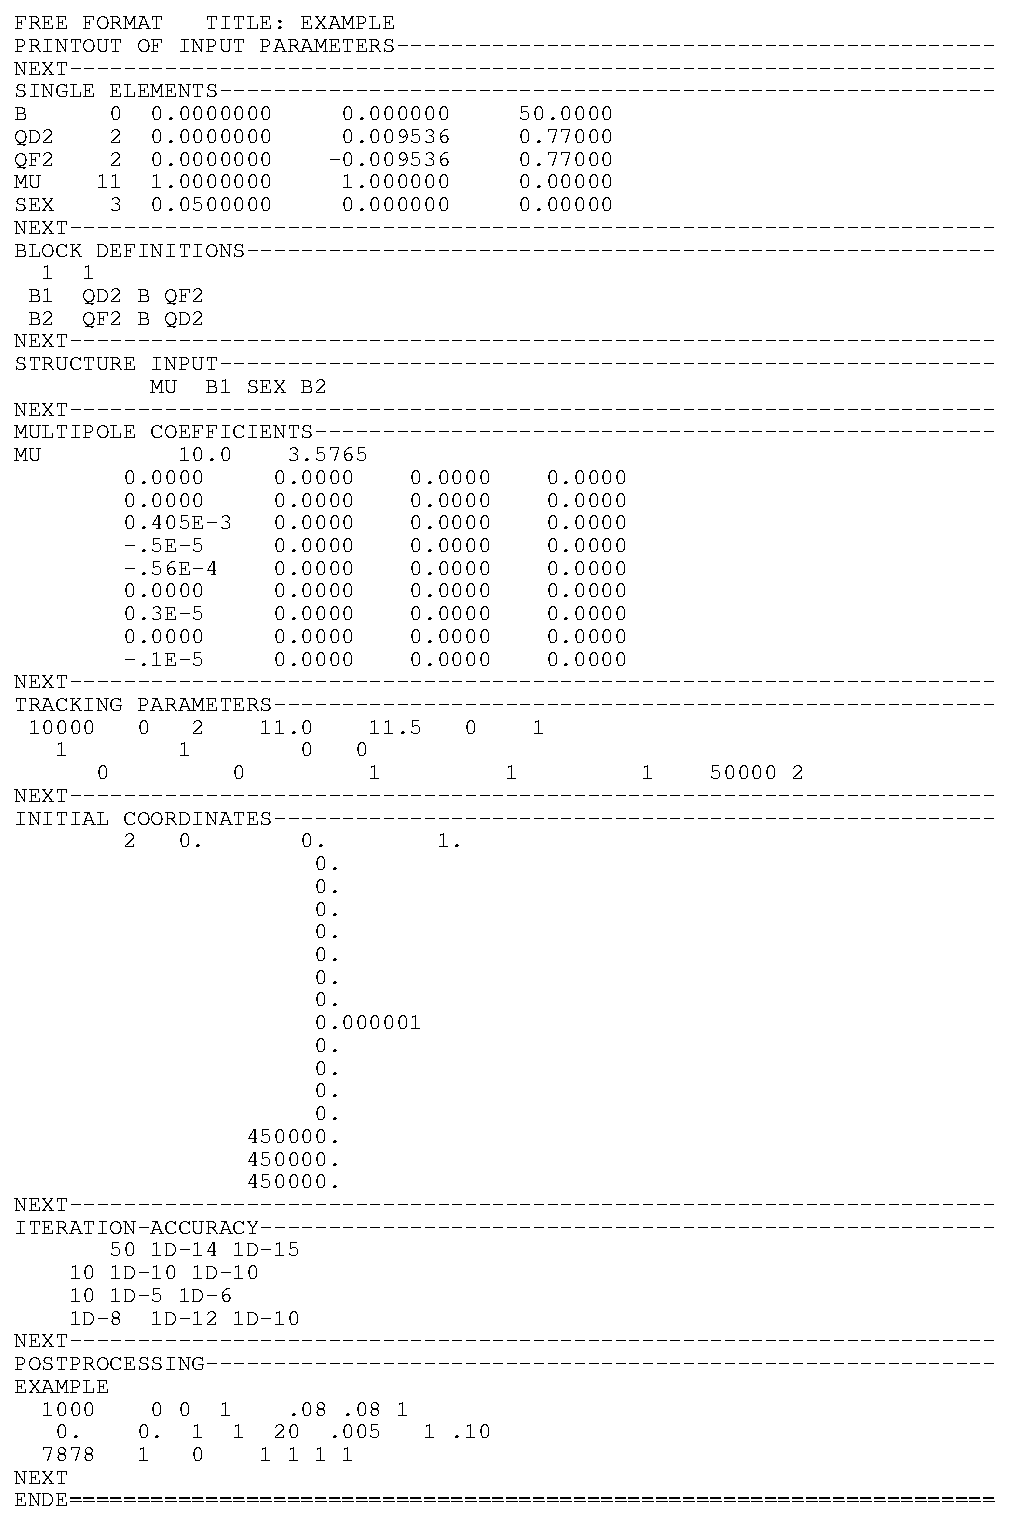
\includegraphics[width=16cm,height=18cm]{expout1}
\end{center}
\end{figure}

\clearpage

\section{Output Example} \label{output}

The preprocessing part is shown first.
\begin{figure}[H]\vspace{-5mm}
\begin{center}
  \mbox{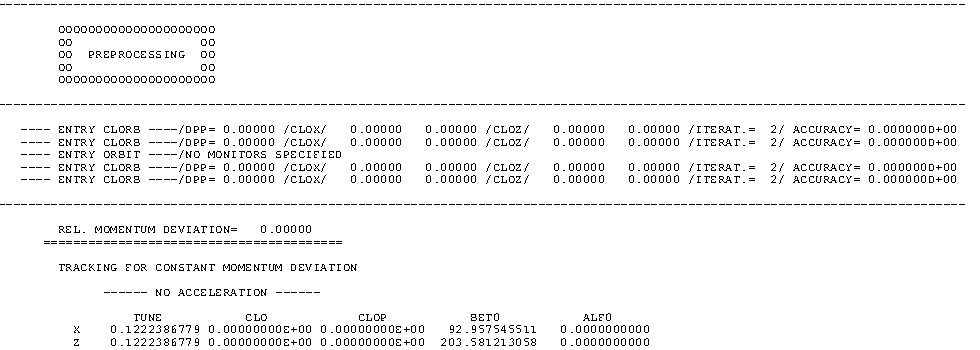
\includegraphics[width=16cm,height=6.5cm]{expout2}}
\end{center}
\end{figure}
Followed by the initial coordinates and the final coordinates for a
regular (right side) and chaotic (left side) case.
\begin{figure}[H]\vspace{-5mm}
\begin{center}
  \mbox{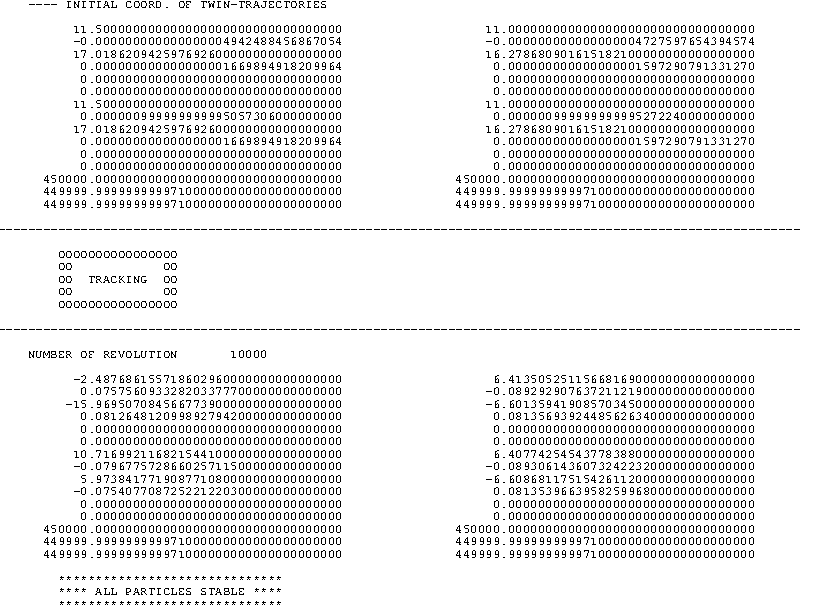
\includegraphics[width=16cm,height=13cm]{expout3}}
\end{center}
\end{figure}

\clearpage

Finally part of the post--processing for the two particles are shown
(chaotic on the left and regular on the right respectively) and a
summary of the post--processing is given.
\begin{figure}[H]
\begin{center}
  \mbox{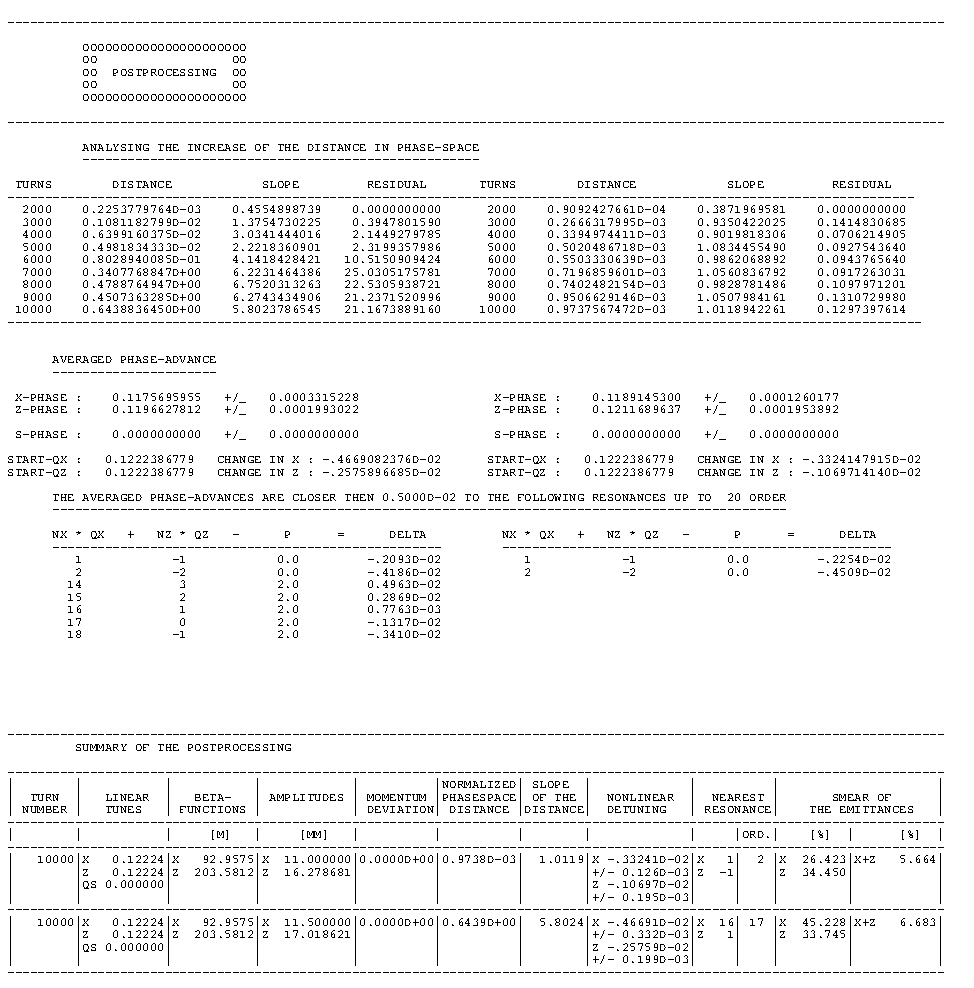
\includegraphics[width=16cm,height=21cm]{expout4}}
\end{center}
\end{figure}

\clearpage

\section{Plot Example} \label{plots}

{\small In figure~\ref{Lya} a typical example of the evolution of the
  distance in phase space is shown of a regular and chaotic particle.
  Figure~\ref{H-proj} and figure~\ref{P-proj} show the corresponding
  horizontal phase space and the physical phase space projections
  respectively. An example of the stroboscoped phase space is shown in
  figure~\ref{P-stro}, where the motion in the chaotic case is beyond
  a ``separatrix'' in the four--dimensional phase space. Even in the
  FFT (figure~\ref{P-FFT}) one can see the effect of chaotic
  behaviour: it leads to a widening of the lines of the spectrum.}
\begin{figure}[H] \vspace*{-5mm}
\begin{center}
  \mbox{\includegraphics*[width=9.cm]{exp1}}
  \\[5mm]
  \mbox{\includegraphics*[width=9.cm]{exp9}}
 \caption{\small Evolution of the Distance of Phase Space for Regular
   \mbox{(upper part)} and Chaotic \mbox{(lower part)} Motion.}
 \label{Lya}
\end{center}
\end{figure} 

\begin{figure}[H]
\begin{center}
  \mbox{\includegraphics*[width=10.5cm]{exp2}}
  \\[5mm]
  \mbox{\includegraphics*[width=10.5cm]{exp10}}
 \caption{Horizontal Phase Space Projections for the
   Regular (upper part) and the Chaotic \mbox{(lower part)} Cases.}
 \label{H-proj}
\end{center}
\end{figure}

\begin{figure}[H]
\begin{center}
  \mbox{\includegraphics*[width=10.5cm]{exp4}}
  \\[5mm]
  \mbox{\includegraphics*[width=10.5cm]{exp12}}
 \caption{Physical Phase Space Projections for the Regular
   \mbox{(upper part)} and the Chaotic \mbox{(lower part)} Cases.}
 \label{P-proj}
\end{center}
\end{figure}

\begin{figure}[H]
\begin{center}
  \mbox{\includegraphics*[width=10.5cm]{exp6}}
  \\[5mm]
  \mbox{\includegraphics*[width=10.5cm]{exp14}}
 \caption{\small{Stroboscoped Vertical Phase Space Projections
     for the Regular (upper part) and the Chaotic (lower part) Cases
     respectively.  The regular motion stays inside a ``separatrix''
     with two unstable fix--points visible, while the chaotic motion
     is clearly outside this ``separatrix''.}}
 \label{P-stro}
\end{center}
\end{figure}

\begin{figure}[H]
\begin{center}
  \mbox{\includegraphics*[width=10.5cm]{exp7}}
  \\[5mm]
  \mbox{\includegraphics*[width=10.5cm]{exp15}}
 \caption{Horizontal FFT--Analysis for the Regular (upper part)
   and the Chaotic (lower part) Cases.}
 \label{P-FFT}
\end{center}
\end{figure}

\begin{thebibliography}{99}
%
\bibitem{DALIE} LBL diffential algebra package and LieLib routines
  courtesy of \'{E}.~Forest. 
%
\bibitem{Ripken95} G.~Ripken and F.~Schmidt, ``A symplectic
  six--dimensional thin--lens formalism for tracking'', CERN SL 95--12
  (AP)(1995), DESY 95--063 (1995).  
  G.~Ripken and F.~Schmidt, ``Construction of Nonlinear Symplectic
  Six--Dimensional Thin--Lens Maps by Exponentiation'', DESY 95--189
  (1995),
  \htmladdnormallink{http://cern.ch/Frank.Schmidt/report/ripken2.pdf}
%  \url{http://cern.ch/Frank.Schmidt/report/ripken2.pdf}
  {http://cern.ch/Frank.Schmidt/report/ripken2.pdf}; D.P.~Barber,
  K.~Heinemann, G.~Ripken and F.~Schmidt, ``Symplectic Thin\,-\,Lens
  Transfer Maps for SixTrack: Treatment of Bending Magnets in Terms of
  the Exact Hamiltonian'', DESY 96--156 (1995),
  \htmladdnormallink{http://cern.ch/Frank.Schmidt/report/ripken3.pdf}
  {http://cern.ch/Frank.Schmidt/report/ripken3.pdf}.  
%
\bibitem{RACETRACK} A.~Wrulich, ``RACETRACK, A computer code for the
  simulation of nonlinear motion in accelerators'', DESY 84--026
  (1984).  
%
\bibitem{FASTRAC} B.~Leemann and \'{E}.~Forest, ``Brief
  description of the tracking codes FASTRAC and THINTRAC'', SSC Note
  SSC--133.  
%
\bibitem{Ripken85} G.~Ripken, ``Nonlinear canonical
  equations of coupled synchro--betatron motion and their solution
  within the framework of a nonlinear 6--dimensional (symplectic)
  tracking program for ultra--relativistic protons'', DESY 85--084
  (1985).  
%
\bibitem{Ripken87} D.P.~Barber, G.~Ripken and F.~Schmidt,
  ``A nonlinear canonical formalism for the coupled
  synchro--betatron motion of protons with arbitrary energy'', DESY
  87--036 (1987); G.~Ripken and F.~Schmidt, ``A symplectic
  six--dimensional thin--lens formalism for tracking'', CERN/SL/95--12
  (AP), DESY 95--063 (1995),
  \htmladdnormallink{http://cern.ch/Frank.Schmidt/report/ripken.pdf}
  {http://cern.ch/Frank.Schmidt/report/ripken.pdf}; K.~Heinemann,
%
\bibitem{HBOOK}
  R.~Brun and D.~Lienart, ``HBOOK User Guide'', CERN Program Library
  Y250 (1987).  
%
\bibitem{HPLOT} R.~Brun and N.C.~Somon, ``HPLOT User
  Guide'', CERN Program Library Y251 (1988).  
%
\bibitem{HIGZ} R.~Bock,
  R.~Brun, O.~Couet, N.C.~Somon, C.E. Vandoni and P. Zanarini, ``HIGZ
  User Guide'', CERN Program Library Q120.  
%
\bibitem{Gilbert78}
  G.~Guignard, ``A general treatment of resonances in accelerators'',
  CERN 78--11 (1978).  
%
\bibitem{Berz89} M.~Berz, ``Differential
  algebra description of beam dynamics to very high orders'', Particle
  Accelerators, 1989, Vol. \underline{24}, pp. 109--124.
%
\bibitem{DAFOR} M.~Berz, ``DAFOR -- Differential Algebra Precompiler
  Version 3, Reference Manual'', MSUCL--755 (1991).
%
\bibitem{Sixvec} F.~Schmidt and M.~Vaenttinen, ``Vectorisation of the
  single particle tracking program SixTrack'', CERN SL Note 90--20
  (1990) (AP).  
%
\bibitem{thesis} F.~Schmidt, ``Untersuchungen zur dynamischen
  Akzeptanz von Protonenbeschleunigern und ihre Begrenzung durch
  chaotische Bewegung'', DESY HERA 88--02, (1988).  
%
%\bibitem{Daspeed} J.~Irwin, private communication.
%
\bibitem{CONVERTOR} H.~Grote, ``A MAD--SixTrack interface'', SL Note
  97--02 (AP).  

\bibitem{sixphys} SixTrack Physics Manual, \url{http://sixtrack.web.cern.ch/SixTrack/}

%
\bibitem{Forest89} M.~Berz, \'{E}. Forest
  and J. Irwin, ``Normal form methods for complicated periodic
  systems: a complete solution using differential algebra and lie
  operators'', Particle Accelerators, 1989, Vol. \underline{24}, pp.
  91--107.  
%
\bibitem{BasErs} M.~Bassetti and G.A.~Erskine,
  ``Closed expression for the electrical field of a two--dimensional
  Gaussian charge'', CERN--ISR--TH/80--06.  
%
\bibitem{Hirata} K.~Hirata, H.~Moshammer, F.~Ruggiero and M.~Bassetti,
  ``Synchro-Beam interaction'', CERN SL-AP/90-02 (1990) and Proc.
  Workshop on Beam Dynamics Issues of High-Luminosity Asymmetric
  Collider Rings, Berkeley, 1990, ed. A.M. Sessler (AIP Conf.  Proc.
  214, New York, 1990), pp. 389-404;\\
  K.~Hirata, H.~Moshammer and F.~Ruggiero, ``A symplectic beam-beam
  interaction with energy change'', KEK preprint 92-117 A (1992) and
  Part. Accel. 40, 205-228 (1993);\\
  K.~Hirata, ``BBC User's Guide; A Computer Code for Beam-Beam Interaction 
  with a Crossing Angle, version 3.4'', SL-Note 97-57 AP.
%
\bibitem{ripbeam} L.H.A.~Leunissen, F.~Schmidt and G.~Ripken, ``6D
  Beam--Beam Kick including Coupled Motion'', LHC Project Report 369,
  \htmladdnormallink{http://cern.ch/Frank.Schmidt/report/ripken\_new.pdf}
  {http://cern.ch/Frank.Schmidt/report/ripken\_new.pdf}.
%
\bibitem{SODD} F.~Schmidt, ``SODD:\\ A Computer Code to calculate
  Detuning and Distortion Function Terms in First and Second Order'',
  CERN SL/Note 99--009 (AP),
  \htmladdnormallink{http://cern.ch/Frank.Schmidt/report/sodd\_manual.pdf}
  {http://cern.ch/Frank.Schmidt/report/sodd\_manual.pdf}.
%
\bibitem{MAD}
  H.~Grote and F.C.~Iselin, ``The MAD program (Methodical Accelerator
  Design), Version 8.10, User's Reference Manual'', CERN SL 90--13
  (AP) (Rev. 4)\\
  \htmladdnormallink{http://cern.ch/Hans.Grote/mad/mad8/doc/mad8\_user.ps.gz}
  {http://cern.ch/Hans.Grote/mad/mad8/doc/mad8\_user.ps.gz}.
%
\bibitem{ERIC} private communication.  
%
\bibitem{RANECU} F.~James, ``A review of
  pseudo--random number generators'', to be published in Computer
  Physics Communication.  
%
\bibitem{Auti} B.~Autin and Y.~Marti, ``Closed Orbit Correction of
  A.G. Machines Using a Small Number of Magnets'',
  CERN--ISR--MA/73--17.
%
\bibitem{Massimo} M.~Giovannozzi,
  ``Description of software tools to perform tune--shift correction
  using normal forms'', CERN SL Note 93--111 (AP).
%
\bibitem{Refine} F.~Schmidt, F.~Willeke and F.~Zimmermann,
  ``Comparison of methods to determine long--term stability in proton
  storage rings'', 1991, Particle Accelerators, Vol. \underline{35},
  pp. 249--256.  

\bibitem{plato1} R.~Bartolini, A.~Bazzani, M.~Giovannozzi, W.~Scandale, E.~Todesco,``Tune evaluation in simulations and experiments'',Part. Accel. 52 147

\bibitem{plato2} M.~Giovannozzi, E.~Todesco, A.~Bazzani and R.~Bartolini (1997). ``PLATO: a program library for the analysis of nonlinear betatronic motion'', Nucl. Instrum. and Methods A 388 1

\bibitem{sixdesk1} SixDesk manual, see SixTrack website, \url{http://sixtrack.web.cern.ch/SixTrack/}

\bibitem{sixdesk2} SixDesk manual, \url{https://www.overleaf.com/1345694dwypbp#/3325092/}

%
%\bibitem{PATRAC} A.~Hilaire and A.~Warman, ``A
%  program for single particle tracking'', CERN SPS/88--8 (AMS).
%
\bibitem{DYNKpaper} K.~Sjobak, H.~Burkhardt, R.D.~Maria, A.~Mereghetti and A.~Santamaria,
  ``General functionality for turn-dependent element properties in SixTrack''
  2015, Procedings of IPAC'13, Richmond, VA, USA, May 2015.
%
\bibitem{SRussen:fieldComp} S.~Russenschuck,
  ``Field computation for Accelerator Magnets'',
  Wiley-VCH, 2010
\bibitem{BurlaKing:CurrentRamp} P.~Burla, Q.~King and J.G.~Pett,
  ``Optimisation of the current ramp for the LHC'',
  Proceedings of the 1999 Particle Accelerator Conference, New York, 1999.
  
%
%\addcontentsline{toc}{chapter}{~\reftype}
\addcontentsline{toc}{chapter}{Bibliography}

\end{thebibliography}

\end{document}

% \chapter{MAD SixTrack Convertor} \label{MADSIXC}

% A special version of the MAD program has been generated that creates
% input files for SixTrack with the complete and exact description of
% the current accelerator model stored in MAD\@. This then allows a
% detailed comparison of the tracking results from both programs.

% The programs SixTrack and MAD \cite {MAD} are both used for particle
% tracking in realistic machines such as the LHC with all expected field
% errors up to the highest order, and with displacement errors of
% quadrupoles and possibly other elements. The LHC lattice and error
% description, however, exists only in MAD format due to its much
% greater flexibility and readability. If one wants to compare tracking
% results of the two programs one needs therefore a conversion of the
% current machine inside MAD into SixTrack format. In particular the
% generated random field and displacement errors have to be transmitted
% correctly since they influence the outcome of the long--term tracking
% greatly.

% To this end it was necessary to make a special MAD version that reads
% a machine description, expands it, generates the errors, and then
% performs the necessary transformations for SixTrack: different
% conventions for the signs of magnet forces, grouping of identical
% elements, concatenation of multiple drift spaces, creation of blocks
% of linear elements between nonlinear ones, a different description
% of field and position errors, and similar tedious questions had to be
% solved. The results of the transformation are then written into input
% files for SixTrack.

% The special MAD version is actually a full MAD (except for plotting)
% with an additional module for the SixTrack output.  This then allows
% the user to perform orbit corrections and other calculations inside
% MAD, and have the resulting modifications of the machine be
% transferred to SixTrack.  All position errors (including tilt errors)
% and field errors are transmitted.

% The converter works correctly for thin and thick lens lattices.  In
% the latter case, all dipoles and quadrupoles are split into two, and a
% multipole is inserted in the centre, except for orbit corrector
% magnets which are converted to thin lens.  Since MAD does not support
% field errors higher than third order for thick elements, the
% multipolar errors will have to be created with the corresponding thin
% lens model, or by some other means.

% The special MAD version accepts one additional command:
% \begin{verbatim}
%  sixt:
%       elem       = (up to 20) element names
%       lgelem     = (up to 20) lengths of the above elements
%       structure  = structure file name, default: "fort.2"
%       param_in   = name of a (mandatory, possibly empty)
%                    extra input file for MAD, default: "fort.3.in"
%       param_out  = parameter file name, default: "fort.3"
%       errors     = field errors file name, default: "fort.16"
%       poserr     = position errors file name, default: "fort.8"
%       cavall     = all cavities in the structure, default: one only.
% \end{verbatim}
% The element length facility is necessary to give SixTrack the real
% lengths of the dipoles (and possibly other elements) that are replaced
% by thin multipoles.  \\
% The parameter input file is copied to the start of the parameter
% output file which may be useful in certain situations.
